\documentclass[final]{article}
\usepackage[margin=1in]{geometry}
\usepackage{quantikz}
\usepackage{caption}
\usepackage{float}
\usepackage{tikz}
\usepackage[dvipsnames]{xcolor}
\usepackage{subcaption}
\usetikzlibrary{calc,arrows.meta}
\usepackage{authblk}
\renewcommand\Authfont{\large\bfseries}
\renewcommand\Affilfont{\normalfont\itshape\normalsize}

\usepackage{graphicx} 
\usepackage{amssymb,amsthm}

\DeclareMathOperator{\Tr}{\mathrm{Tr}}

\usetikzlibrary{calc}     

\usepackage{hyperref}
\definecolor{LightBlue}{HTML}{00A6D6} % A standard "LightBlue" RGB
\usepackage{cleveref}

\newtheorem{theorem}{Theorem}[subsection]
\newtheorem{lemma}[theorem]{Lemma}
\newtheorem{cor}{Corollary}[theorem]

\usepackage{xcolor}

% Shared TikZ colors, sizes, and figure macros for all figures.
% ============================================================
% tikz preamble.tex
% Shared TikZ colors, sizes, and figure macros for the whole paper.
% Loaded once from main.tex. Individual figures live in the
% 'fig - ...' files and only use what is defined here.
% ============================================================

% ---------- shared colors ----------
\definecolor{Zcol}{HTML}{FF1744}
\definecolor{Xcol}{HTML}{00B7FF}
\definecolor{HCol}{HTML}{D35400}
\definecolor{SwapCol}{HTML}{8E44AD}
\colorlet{Rcol}{Zcol}
\colorlet{Bcol}{Xcol}
% luminance-balanced stabilizer tints (annotated diagrams, Figure 3)
\colorlet{Xtint}{Xcol!26}
\colorlet{Ztint}{Zcol!17}
% luminance-balanced vivid fills (lattice maps, Figure 2)
\colorlet{Xvivid}{Xcol!95}
\colorlet{Zvivid}{Zcol!50}
\newcommand{\qdLine}{0.7pt}  % qudit circle rim weight

% ---------- shared sizes ----------
\newcommand{\qdR}{4.8pt}      % qudit circle radius
\newcommand{\numFont}{\scriptsize} % numbers inside circles
\newcommand{\labelFont}{\normalsize} % X/Z labels
\newcommand{\arrAngle}{70}    % wedge arrow half-angle
\newcommand{\arrLen}{0.17cm}  % wedge arrow tail length
\newcommand{\edge}{1.20cm}
\newcommand{\thick}{1pt}

% ---------- five-qutrit patch and stabilizer macros (d=2 figure) ----------
% Outlined stabilizer-patch fills used in the d=2 redefined X/Z grids.
% These match the d=3 convention: each stabilizer is shown as a lightly
% filled patch with its own colored perimeter, while X- and Z-type checks
% are drawn on separate copies of the lattice.
\newcommand{\FiveQBlueTriOutlined}[3]{%
  \path[fill=Xtint,draw=Xcol,line width=1.0pt]
    (#1) -- (#2) -- (#3) -- cycle;
}

\newcommand{\FiveQRedTriOutlined}[3]{%
  \path[fill=Ztint,draw=Zcol,line width=1.0pt]
    (#1) -- (#2) -- (#3) -- cycle;
}

% On the d=2 redefined grids, one stabilizer boundary would otherwise run
% straight through qudit 2 even though qudit 2 is not in that stabilizer.
% These helper paths replace that diagonal by a clean detour around the
% visible q2 silhouette. The blue detour keeps the circular line-around-node
% shape from the previous version. The red detour follows the left outline of
% the q2 arrow/circle silhouette so B_1 reads as bypassing q2 rather than using
% q2.
\newcommand{\FiveQDetourR}{\qdR}
\newcommand{\FiveQArrowTipDetour}{\dimexpr\qdR+\arrLen\relax}
\newcommand{\FiveQDetouredBlueTriQoneQthreeQfour}{%
  % A_2 bypasses q2. Fill the detoured patch, draw the normal boundary, then
  % overdraw only the q2-contacting arc underneath q2 so the visible blue sits
  % flush against the black circle with no white halo.
  \path[fill=Xtint,draw=none,line cap=round,line join=round]
    (q1)
    -- ($(q2)+(45:\FiveQDetourR)$)
    arc[start angle=45,end angle=-135,radius=\FiveQDetourR]
    -- (q3) -- (q4) -- cycle;
  \draw[Xcol,line width=1.0pt,line cap=round,line join=round]
    (q1)
    -- ($(q2)+(45:\FiveQDetourR)$)
    arc[start angle=45,end angle=-135,radius=\FiveQDetourR]
    -- (q3) -- (q4) -- cycle;
  \draw[Xcol,line width=1.8pt,line cap=round,line join=round]
    ($(q2)+(45:\FiveQDetourR)$)
    arc[start angle=45,end angle=-135,radius=\FiveQDetourR];
}
\newcommand{\FiveQDetouredRedTriQzeroQoneQthree}{%
  % B_1 bypasses q2. The contact path exactly follows the q2 silhouette:
  % right wedge base -> wedge tip -> left wedge base -> left-lower circle arc.
  % That contact path is overdrawn slightly wider underneath q2; after q2 is
  % redrawn, the visible red has zero white gap to the black qudit/arrow.
  \path[fill=Ztint,draw=none,line cap=round,line join=round]
    (q0) -- (q1)
    -- ($(q2)+(20:\FiveQDetourR)$)
    -- ($(q2)+(90:\FiveQArrowTipDetour)$)
    -- ($(q2)+(160:\FiveQDetourR)$)
    arc[start angle=160,end angle=225,radius=\FiveQDetourR]
    -- (q3) -- cycle;
  \draw[Zcol,line width=1.0pt,line cap=round,line join=round]
    (q0) -- (q1)
    -- ($(q2)+(20:\FiveQDetourR)$)
    -- ($(q2)+(90:\FiveQArrowTipDetour)$)
    -- ($(q2)+(160:\FiveQDetourR)$)
    arc[start angle=160,end angle=225,radius=\FiveQDetourR]
    -- (q3) -- cycle;
  \draw[Zcol,line width=1.8pt,line cap=round,line join=round]
    ($(q2)+(20:\FiveQDetourR)$)
    -- ($(q2)+(90:\FiveQArrowTipDetour)$)
    -- ($(q2)+(160:\FiveQDetourR)$)
    arc[start angle=160,end angle=225,radius=\FiveQDetourR];
}

% === AUTO-GENERATED routed stabilizer macros (d=2) ===
%% AUTO-GENERATED d=2 routed stabilizers
\newcommand{\FiveQRouteX}{%
  \path[fill=Xtint,draw=none] (0.0000,0.0000)--(1.0000,1.0000)--(-1.0000,1.0000)--cycle;
  \path[fill=Xtint,draw=none] (-1.0000,-1.0000)--(1.0000,-1.0000)--(1.0000,1.0000)--(0.1423,0.1423)--(0.1492,0.1309)--(0.1559,0.1197)--(0.1625,0.1085)--(0.1688,0.0975)--(0.1751,0.0863)--(0.1812,0.0751)--(0.1868,0.0634)--(0.1905,0.0510)--(0.1934,0.0385)--(0.1955,0.0257)--(0.1968,0.0129)--(0.1972,0.0000)--(0.1968,-0.0129)--(0.1955,-0.0257)--(0.1934,-0.0385)--(0.1905,-0.0510)--(0.1868,-0.0634)--(0.1822,-0.0755)--(0.1769,-0.0872)--(0.1708,-0.0986)--(0.1640,-0.1096)--(0.1565,-0.1201)--(0.1483,-0.1300)--(0.1395,-0.1395)--(0.1300,-0.1483)--(0.1201,-0.1565)--(0.1096,-0.1640)--(0.0986,-0.1708)--(0.0872,-0.1769)--(0.0755,-0.1822)--(0.0634,-0.1868)--(0.0510,-0.1905)--(0.0385,-0.1934)--(0.0257,-0.1955)--(0.0129,-0.1968)--(0.0000,-0.1972)--(-0.0129,-0.1968)--(-0.0257,-0.1955)--(-0.0385,-0.1934)--(-0.0510,-0.1905)--(-0.0634,-0.1868)--(-0.0755,-0.1822)--(-0.0872,-0.1769)--(-0.0986,-0.1708)--(-0.1096,-0.1640)--(-0.1201,-0.1565)--(-0.1300,-0.1483)--(-0.1395,-0.1395)--cycle;
  \draw[Xcol,line width=1.0pt,line cap=round,line join=round] (0.0000,0.0000) -- (1.0000,1.0000) -- (-1.0000,1.0000) -- cycle;
  \draw[Xcol,line width=1.0pt,line cap=round,line join=round] (-1.0000,-1.0000) -- (1.0000,-1.0000) -- (1.0000,1.0000) -- (0.1423,0.1423) -- (0.1492,0.1309) -- (0.1559,0.1197) -- (0.1625,0.1085) -- (0.1688,0.0975) -- (0.1751,0.0863) -- (0.1812,0.0751) -- (0.1868,0.0634) -- (0.1905,0.0510) -- (0.1934,0.0385) -- (0.1955,0.0257) -- (0.1968,0.0129) -- (0.1972,0.0000) -- (0.1968,-0.0129) -- (0.1955,-0.0257) -- (0.1934,-0.0385) -- (0.1905,-0.0510) -- (0.1868,-0.0634) -- (0.1822,-0.0755) -- (0.1769,-0.0872) -- (0.1708,-0.0986) -- (0.1640,-0.1096) -- (0.1565,-0.1201) -- (0.1483,-0.1300) -- (0.1395,-0.1395) -- (0.1300,-0.1483) -- (0.1201,-0.1565) -- (0.1096,-0.1640) -- (0.0986,-0.1708) -- (0.0872,-0.1769) -- (0.0755,-0.1822) -- (0.0634,-0.1868) -- (0.0510,-0.1905) -- (0.0385,-0.1934) -- (0.0257,-0.1955) -- (0.0129,-0.1968) -- (0.0000,-0.1972) -- (-0.0129,-0.1968) -- (-0.0257,-0.1955) -- (-0.0385,-0.1934) -- (-0.0510,-0.1905) -- (-0.0634,-0.1868) -- (-0.0755,-0.1822) -- (-0.0872,-0.1769) -- (-0.0986,-0.1708) -- (-0.1096,-0.1640) -- (-0.1201,-0.1565) -- (-0.1300,-0.1483) -- (-0.1395,-0.1395) -- cycle;
}
\newcommand{\FiveQRouteZ}{%
  \path[fill=Ztint,draw=none] (-1.0000,-1.0000)--(-0.1395,-0.1395)--(-0.1483,-0.1300)--(-0.1565,-0.1201)--(-0.1640,-0.1096)--(-0.1708,-0.0986)--(-0.1769,-0.0872)--(-0.1822,-0.0755)--(-0.1868,-0.0634)--(-0.1905,-0.0510)--(-0.1934,-0.0385)--(-0.1955,-0.0257)--(-0.1968,-0.0129)--(-0.1972,-0.0000)--(-0.1968,0.0129)--(-0.1955,0.0257)--(-0.1934,0.0385)--(-0.1905,0.0510)--(-0.1868,0.0634)--(-0.1812,0.0751)--(-0.1751,0.0863)--(-0.1688,0.0975)--(-0.1625,0.1085)--(-0.1559,0.1197)--(-0.1492,0.1309)--(-0.1423,0.1423)--(-0.1351,0.1540)--(-0.1275,0.1661)--(-0.1194,0.1787)--(-0.1109,0.1921)--(-0.1017,0.2063)--(-0.0918,0.2216)--(-0.0809,0.2385)--(-0.0689,0.2572)--(-0.0554,0.2784)--(-0.0399,0.3029)--(-0.0218,0.3319)--(-0.0000,0.3672)--(0.0218,0.3319)--(0.0399,0.3029)--(0.0554,0.2784)--(0.0689,0.2572)--(0.0809,0.2385)--(0.0918,0.2216)--(0.1017,0.2063)--(0.1109,0.1921)--(0.1194,0.1787)--(0.1275,0.1661)--(0.1351,0.1540)--(0.1423,0.1423)--(1.0000,1.0000)--(-1.0000,1.0000)--cycle;
  \path[fill=Ztint,draw=none] (1.0000,-1.0000)--(1.0000,1.0000)--(0.0000,0.0000)--cycle;
  \draw[Zcol,line width=1.0pt,line cap=round,line join=round] (-1.0000,-1.0000) -- (-0.1395,-0.1395) -- (-0.1483,-0.1300) -- (-0.1565,-0.1201) -- (-0.1640,-0.1096) -- (-0.1708,-0.0986) -- (-0.1769,-0.0872) -- (-0.1822,-0.0755) -- (-0.1868,-0.0634) -- (-0.1905,-0.0510) -- (-0.1934,-0.0385) -- (-0.1955,-0.0257) -- (-0.1968,-0.0129) -- (-0.1972,-0.0000) -- (-0.1968,0.0129) -- (-0.1955,0.0257) -- (-0.1934,0.0385) -- (-0.1905,0.0510) -- (-0.1868,0.0634) -- (-0.1812,0.0751) -- (-0.1751,0.0863) -- (-0.1688,0.0975) -- (-0.1625,0.1085) -- (-0.1559,0.1197) -- (-0.1492,0.1309) -- (-0.1423,0.1423) -- (-0.1351,0.1540) -- (-0.1275,0.1661) -- (-0.1194,0.1787) -- (-0.1109,0.1921) -- (-0.1017,0.2063) -- (-0.0918,0.2216) -- (-0.0809,0.2385) -- (-0.0689,0.2572) -- (-0.0554,0.2784) -- (-0.0399,0.3029) -- (-0.0218,0.3319) -- (-0.0000,0.3672) -- (0.0218,0.3319) -- (0.0399,0.3029) -- (0.0554,0.2784) -- (0.0689,0.2572) -- (0.0809,0.2385) -- (0.0918,0.2216) -- (0.1017,0.2063) -- (0.1109,0.1921) -- (0.1194,0.1787) -- (0.1275,0.1661) -- (0.1351,0.1540) -- (0.1423,0.1423) -- (1.0000,1.0000) -- (-1.0000,1.0000) -- cycle;
  \draw[Zcol,line width=1.0pt,line cap=round,line join=round] (1.0000,-1.0000) -- (1.0000,1.0000) -- (0.0000,0.0000) -- cycle;
}
% === end routed macros ===

\newcommand{\FiveQPatchRedefinedXGrid}{%
  \def\L{1.0}
  \coordinate (q0) at (-\L, \L); \coordinate (q1) at ( \L, \L);
  \coordinate (q2) at ( 0 , 0 );
  \coordinate (q3) at (-\L,-\L); \coordinate (q4) at ( \L,-\L);
  \FiveQRouteX
  \FiveQPatchEdges
}

\newcommand{\FiveQPatchRedefinedZGrid}{%
  \def\L{1.0}
  \coordinate (q0) at (-\L, \L); \coordinate (q1) at ( \L, \L);
  \coordinate (q2) at ( 0 , 0 );
  \coordinate (q3) at (-\L,-\L); \coordinate (q4) at ( \L,-\L);
  \FiveQRouteZ
  \FiveQPatchEdges
}

% standard black wedge arrow
\newcommand{\WedgeArrow}[2]{%
  \path[fill=black,draw=none]
    ($(#1)+({\qdR*cos(#2+\arrAngle)},{\qdR*sin(#2+\arrAngle)})$)
      arc[start angle=#2+\arrAngle, end angle=#2-\arrAngle, radius=\qdR]
      -- ($(#1)+({(\qdR+\arrLen)*cos(#2)},{(\qdR+\arrLen)*sin(#2)})$) -- cycle;
}

% ----- PATCH GEOMETRY -----

% 1. Edges Only
\newcommand{\FiveQPatchEdges}{%
  \def\L{1.0} \def\thick{1.0pt}
  \coordinate (q0) at (-\L, \L); \coordinate (q1) at ( \L, \L);
  \coordinate (q2) at ( 0 , 0 );
  \coordinate (q3) at (-\L,-\L); \coordinate (q4) at ( \L,-\L);
  \draw[line width=\thick] (q0) -- (q1);
  \draw[line width=\thick] (q3) -- (q4);
  \draw[line width=\thick] ( 0,\L) -- (0,-\L);
}

% 2. Filled (Reference)
\newcommand{\FiveQPatchFilled}{%
  \def\L{1.0} \def\thick{1.0pt}
  \coordinate (q0) at (-\L, \L); \coordinate (q1) at ( \L, \L);
  \coordinate (q2) at ( 0 , 0 );
  \coordinate (q3) at (-\L,-\L); \coordinate (q4) at ( \L,-\L);
  \path[fill=Xvivid,draw=none] (q0) -- (q2) -- (q1) -- cycle;
  \path[fill=Xvivid,draw=none] (q3) -- (q2) -- (q4) -- cycle;
  \path[fill=Zvivid,draw=none] (q0) -- (q2) -- (q3) -- cycle;
  \path[fill=Zvivid,draw=none] (q1) -- (q2) -- (q4) -- cycle;
  \draw[line width=\thick] (q0) -- (q1);
  \draw[line width=\thick] (q3) -- (q4);
  \draw[line width=\thick] ( 0,\L) -- (0,-\L);
}

% NEW: 2b. Overlapped Fill
\newcommand{\FiveQPatchOverlapped}{%
  \def\L{1.0} \def\thick{1.0pt}
  \coordinate (q0) at (-\L, \L); \coordinate (q1) at ( \L, \L);
  \coordinate (q2) at ( 0 , 0 );
  \coordinate (q3) at (-\L,-\L); \coordinate (q4) at ( \L,-\L);
  % Fill specific triangles with Blue
  \path[fill=Bcol,opacity=0.55,draw=none] (q0) -- (q2) -- (q3) -- cycle;
  \path[fill=Bcol,opacity=0.55,draw=none] (q2) -- (q3) -- (q4) -- cycle;
  % Fill specific triangles with Red
  \path[fill=Rcol,opacity=0.55,draw=none] (q0) -- (q2) -- (q3) -- cycle;
  \path[fill=Rcol,opacity=0.55,draw=none] (q2) -- (q3) -- (q4) -- cycle;
  % Draw lines
  \draw[line width=\thick] (q0) -- (q1);
  \draw[line width=\thick] (q3) -- (q4);
  \draw[line width=\thick] ( 0,\L) -- (0,-\L);
}

% 3. Circles + Wedges
\newcommand{\FiveQPatchCircles}{%
  \foreach \P/\txt in {q0/0,q1/1,q2/2,q3/3,q4/4}{
    \draw[line width=\qdLine,fill=white] (\P) circle (\qdR);
    \node[font=\numFont] at (\P) {\txt};
  }
  \WedgeArrow{q0}{0}\WedgeArrow{q1}{0}\WedgeArrow{q3}{0}\WedgeArrow{q4}{0}\WedgeArrow{q2}{90}
}

% 3b. Circles + Wedges (Smaller Font for Part d, e, f)
\newcommand{\FiveQPatchCirclesSmall}{%
  \foreach \P/\txt in {q0/0,q1/1,q2/2,q3/3,q4/4}{
    \draw[line width=\qdLine,fill=white] (\P) circle (\qdR);
    \node[font=\numFont] at (\P) {\txt};
  }
  \WedgeArrow{q0}{0}\WedgeArrow{q1}{0}\WedgeArrow{q3}{0}\WedgeArrow{q4}{0}\WedgeArrow{q2}{90}
}

% 4. Circles + Wedges Layered
\newcommand{\FiveQPatchCirclesOneUnderThree}{%
  \foreach \P/\txt in {q0/0,q2/2,q4/4}{
    \draw[line width=\qdLine,fill=white] (\P) circle (\qdR);
    \node[font=\numFont] at (\P) {\txt};
  }
  \def\off{0.10}
  \coordinate (qoneBR) at ($(q3)+(\off,-\off)$);
  \draw[line width=\qdLine,fill=white] (qoneBR) circle (\qdR);
  \node[font=\numFont] at (qoneBR) {1};
  \draw[line width=\qdLine,fill=white] (q3) circle (\qdR);
  \node[font=\numFont] at (q3) {3};
  \WedgeArrow{q0}{0}\WedgeArrow{q3}{0}\WedgeArrow{q4}{0}\WedgeArrow{q2}{90}\WedgeArrow{qoneBR}{0}
}


% --- title block ---
\title{Logical Randomized Benchmarking on a Qutrit Surface Code}

\author[1]{Sohan Ghosh\thanks{\texttt{sohghosh@ucdavis.edu, orcid:0000-0003-1318-5502}}}
\author[2]{Chuan-Hong Liu}
\author[2]{Noah Goss\thanks{\texttt{noahgoss@berkeley.edu}}}
\author[3]{Adeeb Kabir\thanks{\texttt{ask171@scarletmail.rutgers.edu}}}
\author[1]{Aidan Epperly}

\author[3]{Yipeng Huang\thanks{\texttt{}}}
\author[2]{Irfan Siddiqi}
\author[1]{Isaac Kim\thanks{\texttt{ikekim@ucdavis.edu}}}

\affil[1]{Department of Physics and Astronomy, University of California Davis, Davis, CA}
\affil[2]{Quantum Nanoelectronics Laboratory, University of California, Berkeley, CA}
\affil[3]{Department of Computer Science, Rutgers University, New Brunswick, New Jersey}

\newcommand{\ACE}[1]{{\color{red}#1}} % Feel free to move this -Aidan

\date{\today}

\begin{document}
\maketitle

% DRAFT ABSTRACT (2026-10-30): written from the sdim 1.4.0 SI1000/SD6 simulations only.
% Revise before submission, and extend once IQM hardware results exist.
\begin{abstract}
We benchmark logical Clifford gates on a qutrit encoded in the $[[5,1,2]]_3$ folded qutrit surface code, whose single-qutrit logical Cliffords are transversal and of constant depth. Because the code has distance two, we use logical randomized benchmarking with detection (LRB-D), which replaces error correction by postselection on trivial stabilizer syndromes. We simulate LRB-D with the \texttt{sdim} qudit stabilizer simulator under qutrit generalizations of the SI1000 and SD6 circuit-level noise models and sample every circuit through the exact detector error model of \texttt{sdim}. We compare the postselected logical error with that of physical single-qutrit randomized benchmarking under the same noise model at the same two-qutrit gate error probability $p$.
With one ancilla per stabilizer and postselection after every forward logical Clifford, the logical error is the smaller one up to a pseudo-threshold $p^\star = 0.0292(6)$ under SI1000 and $0.0399(15)$ under SD6.
Near these values almost every shot is rejected at larger depth, so these pseudo-thresholds rest on fits over the depths $m \le 6$ of additional high-$p$ runs.
% p* and their standard errors (seq_boot_se, sequence bootstrap) from LRB-experiment-data-slurm/comparisons/pseudo-thresholds-current.csv; layout gaps, each layout against the RB of its own run, with standard errors added in quadrature: paper-rework/scratch/lead/se_comparisons.py (se_comparisons.out), checked by paper-rework/scratch/writer-seq-se/check.py (check.out)
When only every fourth check round enters the postselection, the pseudo-threshold falls to $0.0132(2)$ under SI1000 and $0.0155(4)$ under SD6. Uncertainties are one standard error.
A layout with relay ancillas for the two boundary stabilizers lowers the pseudo-threshold by about 10\% under SI1000 and by about 20\% under SD6 when every third or fourth check round enters the postselection. When every round or every second round enters, the differences between the layouts stay within about two standard errors, the largest being $9.7 \pm 4.7\%$ under SD6 when every round enters.
The advantage is conditional on acceptance: under SI1000 at $p = 5\times 10^{-3}$ with postselection after every forward Clifford, $98\%$ of shots are rejected by depth 10.
With postselection on a terminal check alone, the accepted logical signal does not decay as a single exponential, and at depth 22 it falls below the physical signal for $p \geq 10^{-2}$ under SI1000 and $p \geq 5\times 10^{-3}$ under SD6.
\end{abstract}

\section{Introduction}\label{sec:intro}

Quantum computations are intrinsically susceptible to noise and hence, quantum error correction (QEC) is essential for achieving fault tolerant quantum computing. The current landscape of the field is changing as it is transitioning from the noisy intermediate scale era towards more concrete demonstrations of fault tolerance. The current paradigm relies on qubit-based codes and architectures but an alternative approach has been proposed in the avenue of qudits. This paper will specifically look at the $q=3$ case of qudits, referred to as qutrits, and will work in the early fault tolerant quantum computing (early-FTQC) regime. At this stage, the goal is to realize small logical qutrits with protection against errors, before full scale QEC is feasible. 

Qutrits are three-level systems that present compelling alternatives for early FTQC research, where the aim is to study encoded logical devices before full error-correction cycles are practical. They display a larger and more connected computational state space than qubits: a single qutrit stores $\log_2 3 \approx 1.585$ bits of quantum information, increasing information density and, in principle, reducing both computational and ancillary overheads. Algorithmic primitives admit direct ternary advantages, for example, base-3 decompositions reduce \emph{(i)} circuit depth and \emph{(ii)} the count of costly entangling/non-Clifford gates in Shor’s modular exponentiation and generalized-Toffoli subroutines \cite{Gokhale2019}. Moreover, implementing the quantum Fourier transform (QFT) directly in \emph{base-3} reduces the register length from \(q_2=\lceil \log_2 N\rceil\) bits to \(q_3=\lceil \log_3 N\rceil\) trits; since a QFT over \(q\) digits uses \(\Theta(q^2)\) controlled rotations / controlled-\(\mathrm{SUM}\) operations, the entangling-gate count (and leading-order depth) drops by a factor \((\log_3 N/\log_2 N)^2 \approx 0.40\) at fixed \(N\), with explicit qudit-QFT circuit constructions given in \cite{PavlidisFloratos2021}. Similarly, Grover's search algorithm implemented with qutrits uses multi-level oracles and diffusion operators, reducing the gate count and circuit depth per iteration on hardware with native qutrit control \cite{Ivanov2012}. Beyond algorithms, higher-dimensional encodings improve quantum communication: in qutrit quantum key distribution (QKD), each carrier can encode more than one bit of key and protocols exhibit higher error tolerance than binary schemes \cite{BechmannPasquinucciPeres2000,Cerf2002}. Higher-dimensional systems strengthen foundational certificates used in quantum communication. With three-level systems, entangled pairs achieve larger violations of the Collins–Gisin–Linden–Massar–Popescu (CGLMP) Bell inequality than any qubit-based test, which increases the noise margin available to device-independent protocols \cite{Collins2002}. Further, qutrits are the smallest systems that can violate the Klyachko–Can–Binicioglu–Shumovsky (KCBS) contextuality inequality, improving robustness in semi-device-independent protocols \cite{Klyachko2008}. Qutrits also provide a natural language for simulating spin-1 and \(\mathrm{SU}(3)\) models and related phenomena, broadening the space of near-term scientific targets \cite{Senko2015}.
From a QEC standpoint, \emph{magic-state distillation} (MSD) in odd prime dimensions is especially attractive: quantum Reed Muller codes provide transversal qutrit gates enabling small block, high rate MSD protocols across all prime \(q\) \cite{CampbellPRX2012}, and working directly with \((q>2)\)-level systems further improves MSD overheads and provides routes to universal non-Clifford gates \cite{CampbellPRL2014}. Despite these advantages, systematic stabilizer-code design and logical benchmarking for qudits remain comparatively underexplored and merit systematic study. These considerations align with hardware reality: superconducting transmons, trapped ions, and photonic platforms natively provide multilevel structure.  Multi-platform demonstrations of coherent qutrit control, randomized benchmarking, and entangling operations now exist \cite{Morvan2021,Ringbauer2022,Goss2024}.

In this work, we employ the $[[5,1,2]]_3$ quantum error detection code to encode logical information. The data-qutrit layout and the logical gates are tailored to the connectivity of IQM’s superconducting Garnet QPU.
% TODO(authors): confirm which ancilla layout the Garnet coupler map supports (one ancilla coupled to all three data qutrits of G1 and G4, or the relay layout).
The syndrome extraction of the two boundary stabilizers needs either an ancilla coupled to all three of their data qutrits, which our one-ancilla layout assumes, or an additional relay ancilla, which our two-ancilla layout adds (\autoref{sub:ancilla_layouts}). We characterize the code and its constant-depth transversal logical Clifford gates with the \texttt{sdim} qudit stabilizer simulator \cite{sdim}, establishing a numerical baseline prior to hardware execution. Since the distance $d=2$ code supports error detection but not faithful correction, we adapt standard protocols to Logical Randomized Benchmarking with Detection (LRB-D), which isolates logical performance by postselecting on trivial syndromes. We simulate LRB-D under two circuit-level noise models of Gidney et al.~\cite{GidneyHoneycomb2021} that we generalize to qutrits: the superconducting-inspired SI1000 model and the uniform SD6 model, both parameterized by the two-qutrit gate error probability $p$. Every circuit is sampled through the exact detector error model of \texttt{sdim}, which reaches the $3\times 10^{7}$ shots per depth point that heavy postselection demands. Our objective is to compare the average fidelity of postselected logical Cliffords with that of physical single-qutrit Cliffords under the same noise model at the same $p$. We locate the pseudo-threshold $p^\star(k)$ below which the logical error is the smaller one, as a function of the interval $k$ between the check rounds whose syndromes enter the postselection. We do so for two syndrome-extraction layouts: one ancilla per stabilizer (9 qutrits), and a layout that adds a relay ancilla to each of the two boundary stabilizers (11 qutrits).

% p* and their standard errors (seq_boot_se, sequence bootstrap) from LRB-experiment-data-slurm/comparisons/pseudo-thresholds-current.csv; layout gaps, each layout against the RB of its own run, with standard errors added in quadrature: paper-rework/scratch/lead/se_comparisons.py (se_comparisons.out), checked by paper-rework/scratch/writer-seq-se/check.py (check.out)
With one ancilla per stabilizer and postselection after every forward logical Clifford ($k=1$), we find $p^\star(1) = 0.0292(6)$ under SI1000 and $p^\star(1) = 0.0399(15)$ under SD6, where the parentheses give one standard error from a bootstrap over the random Clifford sequences (\autoref{sub:pseudo_thresholds}).
Near these values almost every shot is rejected at larger depth. The pseudo-thresholds of both models therefore use additional runs at high $p$, at $p \geq 0.015$ under SI1000 and $p \geq 0.025$ under SD6, with $2\times 10^{7}$ shots per sequence and depth on the depths $0, 1, 2, 3, 4$ and $6$, of which the fits for $k \ge 2$ use the even ones (\autoref{sub:results_setup}).
At $p = 10^{-3}$ the logical error per unit depth is more than 90 times smaller than the physical one under both models. The SI1000 comparison is the stricter one, because there the one-qutrit gates of the physical baseline fail with probability $p/10$ rather than $p$. The pseudo-threshold decreases as fewer rounds enter the postselection, to $p^\star(4) = 0.0132(2)$ under SI1000 and $0.0155(4)$ under SD6.
These gains hold conditional on acceptance, and the acceptance probability falls quickly with depth. Under SI1000 at $p = 5\times 10^{-3}$ and $k = 1$, $63\%$ of shots are rejected at depth $m = 2$ and $98\%$ at $m = 10$.
The two-ancilla layout gives lower pseudo-thresholds at $k = 3$ and $4$, by about 10\% under SI1000 and about 20\% under SD6, where each layout is compared with the RB baseline of its own run (\autoref{sub:layout_comparison}). At $k = 1$ and $2$ the gaps are $1.4 \pm 2.9\%$ and $4.5 \pm 2.9\%$ under SI1000 and $9.7 \pm 4.7\%$ and $6.6 \pm 6.3\%$ under SD6. They lie within about two standard errors, and there we do not resolve a difference between the layouts.

Logical dynamics can be non-Markovian even under Markovian physical noise, because the encoded state couples to syndrome subspaces in which undetected errors persist and act on later logical gates \cite{Ziyad2025}. Intermediate postselection discards the trajectories in which a check round detects such an excursion. Our simulations are consistent with this picture, but they do not isolate the mechanism. With terminal postselection alone, the accepted logical signal is not a single exponential in depth: it decays slowly at small depth and then steepens. At depth $m = 22$ it drops below the physical RB signal for $p \geq 10^{-2}$ under SI1000 and for $p \geq 5\times 10^{-3}$ under SD6. Under SI1000 a single exponential describes the accepted decays for $k = 1$ to $4$, closely for $k \le 2$ and approximately for $k = 3$ and $4$, where the traces show small steps at depths that are not multiples of $k$ (\autoref{sub:interval_results}). Under SD6 the accepted decay already steepens with depth at $k = 1$, and under both models the $\chi^2$ of the fit tends to grow with $k$ (\autoref{sub:interval_results}). For $p \geq 0.02$ and $k \le 4$ the exponential form can be tested only over short depths, because almost all shots at large depth are rejected. Each fit of the production runs there rests on two to five depths, and the fits of the high-$p$ runs use at most six depths at $k = 1$ and at most the four even depths at $k \ge 2$, all with $m \le 6$.

\section{Background}\label{sec:bg}

\subsection{Qudit Pauli Group}
For a prime $q$-dimensional quantum system, a qudit, the Pauli group $\mathcal{P}_q$ is defined as the group of unitary error operators generated by the generalized $X$ and $Z$ gates. They form a set of elementary operations and a discrete basis for arbitrary errors \cite{Gottesman1999,Hostens2005,Wang2020,SarkarYoder2024}.
The generators obey the shift and phase action on the computational basis $|j\rangle$ where $j\in\{0,\ldots,q-1\}$:

\begin{itemize}
    \item $X$ (shift operator): $X|j\rangle = |(j+1)\bmod q\rangle$.

    \item $Z$ (phase operator): $Z|j\rangle = \omega^j|j\rangle$,
    where $\omega = e^{2\pi i/q}$ is a primitive $q$th root of unity.
\end{itemize}

Formally, the single-qudit Pauli group is the finite subgroup of $\mathrm{U}(q)$ generated by $X$ and $Z$ together with the global phase
$\omega I$:
\begin{equation}
  \mathcal{P}_q
  := \bigl\{\, \omega^c X^a Z^b : a,b,c \in \mathbb{Z}_q \,\bigr\},
\end{equation}
where $\mathbb{Z}_q = \{0,1,\dots,q-1\}$ denotes integers modulo $q$ and $I$ is the $q\times q$ identity operator.

By construction $X^q = Z^q = I$, and $X^a Z^b = \omega^{-ab}\, Z^b X^a$ for any integers $a,b \in \mathbb{Z}_q$. In particular, $Z X = \omega\, X Z$, so $X$ and $Z$ commute up to the
phase $\omega$. All other Pauli operators, including analogs of the qubit $Y$, can be expressed, up to a global phase, as $X^a Z^b$ for
some $a,b\in \mathbb{Z}_q$. In fact, every element of $\mathcal{P}_q$ equals $\omega^c X^a Z^b$ for a unique tuple $(a,b,c)\in \mathbb{Z}_q^3$.

For an $n$-qudit system, the $n$-qudit Pauli group is
\begin{equation}
  \mathcal{P}_q^{\otimes n}
  := \bigl\{\, \omega^c
      X_1^{a_1} \cdots X_n^{a_n}\,
      Z_1^{b_1} \cdots Z_n^{b_n}
      : \mathbf{a},\mathbf{b} \in \mathbb{Z}_q^n,\;
        c \in \mathbb{Z}_q
     \,\bigr\},
\end{equation}
where $X_k$ and $Z_k$ act as $X$ and $Z$ on the $k$th qudit and as the identity on all others, and
$\mathbf{a}=(a_1,\dots,a_n)$, $\mathbf{b}=(b_1,\dots,b_n)$.
These $n$-fold tensor products of single-qudit Paulis are often called \emph{Pauli strings} \cite{Hostens2005,SarkarYoder2024}.

\subsection{Qudit Clifford Group}

The Qudit Clifford group $\mathcal{C}_q$ is the normalizer of the $n$-qudit Pauli group $\mathcal{P}_q^{\otimes n}$ within the unitary group $U(q^n)$. It is defined as the set of operations that map Pauli operators to Pauli operators under conjugation \cite{Gottesman1999}:
\begin{equation}
    \mathcal{C}_q = \{ U \in U(q^n) \mid U \mathcal{P}_q^{\otimes n} U^\dagger = \mathcal{P}_q^{\otimes n} \}
\end{equation}
This property is central to the Gottesman-Knill theorem, which states that quantum circuits composed solely of Clifford gates and Pauli measurements can be efficiently simulated on a classical computer \cite{Gottesman1998}.

For a prime dimension $q$, the Clifford group is generated by three elementary gates: the Hadamard gate $H$, the Phase gate $S$, and the two-qudit $SUM$ gate (generalizing the qubit CNOT) \cite{Hostens2005}.

\subsubsection{Generators and Conjugation Rules}
The action of these generators on the computational basis and their conjugation effects on the Pauli operators are defined as follows:

\textbf{1. The Hadamard Gate ($H$)} \\
The Hadamard gate implements a Discrete Fourier Transform over $\mathbb{Z}_q$, changing the basis from computational ($Z$) to conjugate ($X$):
\begin{equation}
    H |j\rangle = \frac{1}{\sqrt{q}} \sum_{k=0}^{q-1} \omega^{jk} |k\rangle
\end{equation}
For arbitrary $q$, its conjugation action rotates the Pauli operators, mapping $X$ to $Z$ and $Z$ to $X^{q-1}$:
\begin{align}
    H X H^\dagger &= Z, \\
    H Z H^\dagger &= X^\dagger = X^{q-1} = X^{-1}
\end{align}

\textbf{2. The Phase Gate ($S$)} \\
The Phase gate applies a quadratic phase to the basis states. For odd prime $q$ (such as qutrits, $q=3$), it is defined as:
\begin{equation}
    S |j\rangle = \omega^{j(j-1)/2} |j\rangle
\end{equation}
For $q=3$ this gives $S=\mathrm{diag}(1,1,\omega)$. The \texttt{sdim} simulator calls this gate \texttt{P}.
This gate preserves $Z$ operators but mixes $X$ and $Z$:
\begin{align}
    S X S^\dagger &= X Z, \\
    S Z S^\dagger &= Z
\end{align}

\textbf{3. The Sum Gate ($SUM$)} \\
The $SUM$ gate is the canonical two-qudit entangling gate, generalizing the CNOT. It adds the state of the control qudit ($c$) to the target qudit ($t$) modulo $q$:
\begin{equation}
    SUM (|j\rangle_c \otimes |k\rangle_t)= |j\rangle_c \otimes |(j+k) \bmod q\rangle_t.
\end{equation}
The conjugation rules describe the propagation of errors between qudits:
\begin{align}
    SUM (X \otimes I) SUM^\dagger &= X \otimes X, \\
    SUM (I \otimes X) SUM^\dagger &= I \otimes X, \\
    SUM (Z \otimes I) SUM^\dagger &= Z \otimes I, \\
    SUM (I \otimes Z) SUM^\dagger &= Z^{-1} \otimes Z
\end{align}
Note the appearance of $Z^{-1}$ on the control qudit when a $Z$ error propagates from the target, a distinct feature of qudit stabilizer logic ($q>2$) compared to qubits.

\textbf{4. The Controlled-Phase Gate ($CZ$)} \\
The controlled-phase gate used in the logical $\bar S$ gate follows from the generators. It is diagonal:
\begin{equation}
    CZ = (I\otimes H)\,SUM\,(I\otimes H^\dagger), \qquad
    CZ (|j\rangle \otimes |k\rangle) = \omega^{jk}\, |j\rangle \otimes |k\rangle,
\end{equation}
so it leaves $Z\otimes I$ and $I\otimes Z$ unchanged and maps $X\otimes I \mapsto X\otimes Z$ and $I\otimes X \mapsto Z\otimes X$.

\subsection{Randomized Benchmarking}
Randomized Benchmarking (RB) is a Monte Carlo protocol for estimating the average error rate of a set of quantum gates \cite{Magesan2011PRL,Knill2008,Emerson2005}. Originally developed for qubit systems, RB has been generalized to qudits by considering the appropriate Clifford group in higher dimensions, which also form unitary 2-designs \cite{Appleby2005,Dankert2009,Gross2007}. In essence, RB produces a decay parameter $f \in [0,1]$ such that the probability of a circuit returning the correct result after a sequence of gates of length $m$ is approximately
\begin{equation}
F_{seq}(m) = Af^{m} + B,
\label{eq:fseq}
\end{equation}
(for some constant $A$ and $B$), assuming gate independent Markovian errors \cite{Magesan2011PRL,Magesan2012PRA}. This decay is directly related to the average fidelity of the gates; intuitively, $f^m$ represents the fraction of runs that remain error-free after $m$ gates. One of the powerful features of RB is that it is insensitive to the details of the error model when the noise is gate-independent and Markovian: the randomization in the protocol twirls arbitrary errors to an effective depolarizing form giving a single-exponential decay; with mild gate dependence the decay remains approximately exponential, while strong deviations (e.g., drift, non-Markovianity, leakage) can break the single-exponential model \cite{Emerson2005,Wallman2018}. Nonetheless, this relative robustness has been established in prior works, which show that an RB experiment using only Clifford gates with depolarizing noise can accurately capture the performance of a hardware with more general errors, as long as an effective error probability is chosen \cite{Magesan2011PRL,Proctor2019DRB}.

RB protocol for qutrits: At a high level, RB involves applying a random sequence of gates and measuring how often the system returns to a reference state. In the qutrit case, we uniformly sample random elements from the qutrit Clifford group (which normalizes the qutrit Pauli operators) as our gate set \cite{Appleby2005,Morvan2021}. A standard physical-level RB experiment proceeds as follows:

\begin{enumerate}
    \item \textbf{State Preparation:} Initialize the qutrit in a standard basis state (e.g. $|0\rangle$ in the computational basis). This state serves as the reference for the benchmarking experiment.

    \item \textbf{Random Clifford Sequence:} Apply a sequence of $m$ randomly chosen Clifford gates $C_1, C_2, \dots, C_m$ on the qutrit. Each gate in the sequence is followed by a brief period during which the qutrit experiences noise. The reference model for this exposition is the depolarizing channel
    \begin{equation}
        \mathcal{E}_{\mathcal{D}}(\rho)= (1-p_{\mathrm{mix}})\,\rho+\frac{p_{\mathrm{mix}}}{3}\,I
        \label{eq:1-depol}
    \end{equation}
    with some fixed error probability $p_{\mathrm{mix}}$ per gate (gate-independent noise), while the circuit-level noise models we actually sweep in our simulations are defined in \autoref{sub:noise_models}. In a qutrit, this channel replaces the state by the completely mixed state with probability $p_{\mathrm{mix}}$, which is the same as applying a uniformly random non-identity Pauli error with probability $\tfrac{8}{9}p_{\mathrm{mix}}$. This sequence of interleaved gates and errors is illustrated in the RB circuit schematic of \autoref{fig:rb-stacked} (each Clifford gate $C_j$ is immediately followed by a “noise” box) \cite{NielsenChuang2010,Emerson2005}.
    
    We can justify this because the qutrit Clifford group forms a unitary 2-design. Therefore, averaging (“twirling”) any fixed completely positive and trace preserving (CPTP) noise channel $\Lambda$ over random Clifford
    conjugations matches the Haar second moments and symmetrizes its action on the
    traceless subspace, yielding an effective depolarizing channel with the same
    average gate fidelity.\cite{Dankert2009,Gross2007,Appleby2005,Magesan2011PRL,Emerson2005}
    Formally, the Clifford twirl is
    \begin{equation}
        \mathcal{T}_{\mathcal{C}_3}(\Lambda)(\rho)
        = \frac{1}{|\mathcal{C}_3|}\sum_{C\in\mathcal{C}_3}
        C^\dagger\,\Lambda(C\rho C^\dagger)\,C
        = \int_{U(3)} U^\dagger\,\Lambda(U\rho U^\dagger)\,U\,
        d\mu_{\mathrm{Haar}}(U).
    \label{eq:clifford-twirl}
    \end{equation}
    and it has the depolarizing form
    $\mathcal{T}_{\mathcal{C}_3}(\Lambda)(\rho)=\mathcal{E}_{\mathcal{D}}(\rho)$.
    Representation-theoretically, the Clifford twirl decomposes the 
    Pauli transfer matrix representation into two irreducible subspaces: the trivial irrep spanned by the identity and the $(q^{2}\!-\!1)$-dimensional traceless irrep. By Schur’s lemma the twirled channel has block form
    \begin{equation}
        W_{\mathcal{C}_3}\!\big(R_{\Lambda}\big)=
        \begin{bmatrix}
        1 & 0 \\
        0 & f\,\Pi
        \end{bmatrix},
        \qquad
        \big[W_{\mathcal{C}_3}\!\big(R_{\Lambda}\big)\big]^m=
        \begin{bmatrix}
        1 & 0 \\
        0 & f^{m}\,\Pi
        \end{bmatrix},
    \label{eq:twirl_irrep}
    \end{equation}
    where $\Pi$ projects onto the traceless Pauli subspace (dimension $q^{2}{-}1=8$
    for a qutrit). Thus the identity block contributes a constant offset $B$ while
    the traceless block contributes $A\,f^{m}$, giving the single-exponential
    decay in Eq.~\eqref{eq:fseq} and an effective depolarizing channel with
    parameter $f = 1-p_{\mathrm{mix}}$. For the Weyl-form probability $p$ of \autoref{sub:noise_models}, $p_{\mathrm{mix}} = \tfrac{9}{8}p$ and $f = 1 - \tfrac{9}{8}p$.
    

    \item \textbf{Inverting Operation:} After the $m$ random gates, apply the inverse of the overall Clifford operation. That is, classically compute $C_{\text{inv}} = (C_m C_{m-1}\cdots C_1)^{-1}$, and apply this final Clifford gate. In the absence of errors, $C_{\text{inv}}$ should ideally return the qutrit to the initial state $|0\rangle$. Our simulations use a mirror variant of this step instead~\cite{Proctor2022MirrorRB} (\autoref{sub:rb_baseline}): the inverses $C_m^{-1},\dots,C_1^{-1}$ are applied one at a time in reverse order, each as its own noisy Clifford, so a sequence of depth $m$ contains $2m$ noisy Cliffords (\autoref{fig:rb-stacked}).

    \item \textbf{Measurement:} Finally, measure the qutrit in the computational basis. We record whether the outcome is the expected state or an error. By repeating the experiment many times, we can estimate the probability of returning the correct state for that sequence. The expectation value of $Z$ is given by
    \begin{equation}
         \langle Z\rangle = P_{0} + \omega P_{1} + \omega^{2} P_{2},
    \end{equation}
    where $P_j$ are the proportions of classical $j$ readouts for the various shots, which are then weighed by their respective eigenvalues $\omega^j$. In our simulations this final measurement is ideal, and we average the modulus $|\langle Z\rangle|$ of each sequence's estimate over sequences.
\end{enumerate}

\begin{figure}[H]
  \centering
    \begin{quantikz}[column sep=0.22cm]
      \lstick{\textcolor{LightBlue}{$\ket{0}$}} &
        \gate{\textcolor{red}{C_1}} &
        \gate{\textcolor{violet}{\mathcal{N}}} &
        \push{\,\cdots\,} &
        \gate{\textcolor{red}{C_m}} &
        \gate{\textcolor{violet}{\mathcal{N}}} &
        \gate{\textcolor{red}{C_m^{-1}}} &
        \gate{\textcolor{violet}{\mathcal{N}}} &
        \push{\,\cdots\,} &
        \gate{\textcolor{red}{C_1^{-1}}} &
        \gate{\textcolor{violet}{\mathcal{N}}} &
        \meter{}
    \end{quantikz}
  \caption{Physical RB circuit of depth $m$ used as the baseline in our simulations, in the mirror variant of \autoref{sub:rb_baseline}. The qutrit starts in $\ket{0}$. The Cliffords $C_1,\dots,C_m$ are drawn uniformly from the single-qutrit Clifford group (216 elements up to global phase) and are followed by their inverses in reverse order, so the circuit contains $2m$ noisy Cliffords. Each box $\mathcal{N}$ stands for the one-qutrit depolarizing channels that follow every primitive gate of the preceding Clifford, with probability $p/10$ under SI1000 and $p$ under SD6 (\autoref{sub:noise_models}). The final computational-basis measurement is ideal. The standard protocol of the text replaces the inverse half by a single recovery gate $C_{\text{inv}}$.}
  \label{fig:rb-stacked}
\end{figure}

Steps 1–4 are repeated for many independent random sequences at the same length $m$, and then for various sequence lengths $m$. The resulting survival probabilities (fraction of runs yielding the correct outcome) will decline as $m$ increases, since longer sequences give more opportunity for errors. Under the assumption of gate-independent depolarizing noise, this decay in survival probability is exponential in the number of gates \cite{Magesan2011PRL}. The data is fit using Eq.\eqref{eq:fseq}, with $f$ the per-gate decay and $A,B$ absorbing State Preparation and Measurement (SPAM) errors~\cite{Magesan2011PRL,Magesan2012PRA}.
 The decay parameter $f$ is then used to extract the average gate fidelity. For a qutrit, the relationship between $f$ and the average gate fidelity $\bar{F}$ is given by
\begin{equation}
\bar{F} = \frac{(q-1)f + 1}{q},
\label{eq:fbar}
\end{equation}
(with $q=3$ in this case) \cite{Nielsen2002,Magesan2012PRA}. In other words, if $f=1$ the gates are ideal (fidelity 1), whereas if $f$ is significantly less than 1, the gates lose fidelity with each application. By plotting the measured expectation value versus sequence length (circuit depth) and fitting an exponential, one obtains $f$ and thereby quantifies the average error rate per gate. This methodology has become a standard way to benchmark multilevel quantum gates, offering a simple exponential metric of performance even in complex qutrit systems \cite{Morvan2021,Proctor2019DRB}. In summary, RB provides a reliable, dimension-agnostic measure of gate fidelity decay, making it well-suited to characterizing qutrit operations \cite{Magesan2011PRL,Magesan2012PRA}. In the mirror sequences of our simulations, $m$ counts forward Cliffords, so $f$ and $\bar F$ describe one forward Clifford together with its inverse; \autoref{sub:fit_model} gives the fit model we use, which fixes $B=0$.
\subsection{Logical Randomized Benchmarking (LRB)}

Logical Randomized Benchmarking (LRB) extends the RB concept to characterize the error rates at the logical level, after encoding into a quantum error-correcting code. The idea, first proposed by Combes et al. \cite{Combes2017} is to apply random sequences of logical gates on encoded qudits and measure the fidelity of the logical operations. This allows one to assess how much protection the code and any error-correction procedures provide, by comparing the effective logical error rate to the physical error rate. A typical LRB protocol proceeds in the following steps:
\begin{enumerate}
  \item \textbf{Logical State Preparation:}
  Prepare the system in a logical basis state, e.g.\ the logical
  $|\bar{0}\rangle, |\bar{+}\rangle$, etc. state of the code. All stabilizers of the
  code are initially satisfied, so the state lies in the codespace.

  \item \textbf{Random Logical Clifford Sequence:}
  Apply a sequence of random logical Clifford gates \newline $\{\bar{C}_1, \bar{C}_2, \dots, \bar{C}_m\}$. Each $\bar{C}_j$ denotes a Clifford operation on the codespace, which
  in practice is implemented by some sequence of physical operations on
  the underlying qudits.

  \item \textbf{Error Correction After Each Logical Gate:}
  After each logical gate, one can perform error correction, to diagnose and correct any errors using the code’s stabilizer
  measurements before continuing to the next gate. The error correction
  after each logical gate aims to keep the logical state in the
  codespace by defining a faithful recovery map to the appropriate
  codeword.

  \item \textbf{Logical Inverting Operation:}
  After the sequence of $m$ logical Cliffords, apply the logical inverse
  $
    \bar{C}_{\text{inv}} = (\bar{C}_m \cdots \bar{C}_1)^{-1},
  $
  which ideally returns the encoded state to the initial logical state, if there isn't any noise.

  \item \textbf{Logical Measurement:}
  Finally, measure a logical operator (e.g.\ the logical $\bar Z$, logical $\bar X$, etc.) and compare
  the outcome to the initial logical state. If the error-correcting code
  has successfully kept errors at bay, the random sequence followed by
  its inverse will return the logical qudit to the starting state with
  high probability, just as in physical RB.

  \item \textbf{Repetition and Curve Fitting:}
  Repeat the above procedure across many random sequences and sequence
  lengths $m$. For each $m$, estimate the logical survival probability
  (i.e.\ the probability that the final logical measurement agrees with
  the initial state) and fit the data to an exponential decay curve to
  extract a logical decay parameter $f$. The average logical error
  rate per Clifford can then be derived from $f$, analogous
  to the physical case \cite{Magesan2011PRL,Magesan2012PRA,Wallman2018}. However, this is with the assumption that the logical error channels will be Markovian in nature and that the logical decay curves don't display memory-like features.
\end{enumerate}

LRB offers several clear advantages: it directly characterizes the performance of an error-correction implementation at the logical level, avoiding the need to extrapolate from physical error rates, which can radically under- or overestimate logical performance by many orders of magnitude. By operating inside the smaller logical codespace, LRB achieves a drastic reduction in experimental resources while providing more accurate estimates of key performance indicators such as the average probabilities of correctable and uncorrectable errors and the average logical gate error rate. Further, it attempts to incorporate effects of imperfect logical gates, crosstalk, and correlated errors that are often neglected in physical-layer approaches. As the proof of correctness reduces to that of standard RB, the protocol inherits the robustness and many technical refinements of physical RB that is compatible with existing RB-based analysis tools \cite{Combes2017}. 

Similarly, LRB has important limitations: its theoretical guarantees rely on the usual RB
assumptions that the noise on logical Clifford gates is time-independent, Markovian, and gate-independent,
and in addition it requires that syndrome measurement errors be uncorrelated between rounds of error correction. These conditions are only approximately satisfied in realistic devices, and while the protocol can be shown to be robust to small violations, large deviations can compromise the interpretation of the extracted logical parameters. Furthermore, LRB relies on the availability of an implemented code with logical
Clifford gates and syndrome readout, so it is not a substitute for lower-level characterization of the physical hardware \cite{Combes2017}.

The protocol we simulate departs from steps 3 and 4. Because the $[[5,1,2]]_3$ code has distance 2, we replace error correction by postselection on trivial syndromes, and we replace the single logical inverse by a mirror inverse that applies $\bar C_m^{-1},\dots,\bar C_1^{-1}$ one at a time in this order. \autoref{sub:lrb_d} defines the resulting protocol, LRB-D.


\subsection{Modified Qutrit Surface Code - Folded Surface Code}\label{sec: qudit surface code}

Topological surface codes can be generalized from qubits to qudits (dimension $q$) by using qudit Pauli operators as stabilizers. As seen in \autoref{fig:qudit-surface-code}, in a qudit surface code, the lattice is typically composed of data qudits on a 2D grid where one defines two types of stabilizers: tensor products of $X$-type operators (cyclic shift operators mod $q$) and $Z$-type operators (phase operators mod $q$) on a set of neighbouring physical qudits. These stabilizers mutually commute and define a codespace in which a logical qudit can be encoded. 
% ============================================================
% fig - qudit surface code.tex
% Figure: qudit surface code stabilizers and distance-5 patch.
% Shared colors and sizes come from 'tikz preamble.tex'.
% All three panels are drawn at the same scale (\SCscale) with a
% unit lattice cell, so stabilizer close-ups and the full patch
% stay proportional.
% ============================================================

% ---------- local helpers for this figure only ----------
\newcommand{\SCscale}{1.5}
\newcommand{\SCctx}{black!30}          % context lattice edges in close-ups
\newcommand{\SCgrid}{0.9pt}            % lattice line width
\newcommand{\SCctxline}{0.6pt}          % context lattice line width
\newcommand{\SCpatchline}{1.0pt}       % stabilizer patch outline width

% One qudit: white circle + orientation wedge (0 = right, 90 = up).
\newcommand{\SCqudit}[3]{% position, wedge angle, label
  \WedgeArrow{#1}{#2}
  \draw[line width=\qdLine,fill=white] (#1) circle (\qdR);
  \node[font=\numFont] at (#1) {#3};
}

\begin{figure}[H]
  \centering
  \captionsetup[subfigure]{justification=centering}
  % Left column: the two stabilizer close-ups, drawn on a 2x2-cell window.
  \begin{minipage}[t]{0.34\textwidth}
    \vspace{0pt}
    % -------- (a) Vertex / X-type check --------
    \begin{subfigure}[t]{\linewidth}
      \centering
      \begin{tikzpicture}[line cap=round,line join=round,scale=\SCscale]
        % context lattice
        \foreach \y in {0,1,2} \draw[\SCctx,line width=\SCctxline] (0,\y) -- (2,\y);
        \foreach \x in {0,1,2} \draw[\SCctx,line width=\SCctxline] (\x,0) -- (\x,2);
        % stabilizer patch: diamond over the four edge midpoints
        \path[fill=Xvivid,draw=Xcol!55!black,line width=\SCpatchline]
          (1,1.5) -- (1.5,1) -- (1,0.5) -- (0.5,1) -- cycle;
        % the four edges of the central vertex, at full strength
        \draw[line width=\SCgrid] (0,1) -- (2,1);
        \draw[line width=\SCgrid] (1,0) -- (1,2);
        % qudits
        \SCqudit{1,1.5}{90}{n}
        \SCqudit{1.5,1}{0}{e}
        \SCqudit{1,0.5}{90}{s}
        \SCqudit{0.5,1}{0}{w}
      \end{tikzpicture}
      \caption{Vertex stabilizer generator \mbox{$G_X=X^{\dagger}_n \otimes X_w \otimes X^{\dagger}_e \otimes X_s$}.}
      \label{fig:vertex}
    \end{subfigure}

    \vspace{1.2ex}

    % -------- (b) Face / Z-type check --------
    \begin{subfigure}[t]{\linewidth}
      \centering
      \begin{tikzpicture}[line cap=round,line join=round,scale=\SCscale]
        % context lattice: neighboring edges plus the window frame
        \foreach \y in {0.5,1.5} \draw[\SCctx,line width=\SCctxline] (0,\y) -- (2,\y);
        \foreach \x in {0.5,1.5} \draw[\SCctx,line width=\SCctxline] (\x,0) -- (\x,2);
        \draw[\SCctx,line width=\SCctxline] (0,0) rectangle (2,2);
        % stabilizer patch: diamond over the four edge midpoints of the face
        \path[fill=Zvivid,draw=Zcol!60!black,line width=\SCpatchline]
          (1,1.5) -- (1.5,1) -- (1,0.5) -- (0.5,1) -- cycle;
        % the face itself, at full strength
        \draw[line width=\SCgrid] (0.5,0.5) rectangle (1.5,1.5);
        % qudits
        \SCqudit{1,1.5}{0}{n}
        \SCqudit{1.5,1}{90}{e}
        \SCqudit{1,0.5}{0}{s}
        \SCqudit{0.5,1}{90}{w}
      \end{tikzpicture}
      \caption{Face stabilizer generator \mbox{$G_Z = Z_n \otimes Z_w \otimes Z^{\dagger}_e \otimes Z^{\dagger}_s$}.}
      \label{fig:face}
    \end{subfigure}
  \end{minipage}
  \hfill
  % Right column: the distance-5 patch at the same scale.
  \begin{minipage}[t]{0.62\textwidth}
    \vspace{0pt}
    \begin{subfigure}[t]{\linewidth}
      \centering
      \begin{tikzpicture}[line cap=round,line join=round,scale=\SCscale]
        \newcommand{\nCols}{5}
        \newcommand{\nRows}{5}
        \newcommand{\xLabelOffset}{0.52}
        \newcommand{\zLabelDy}{0.42}

        % top X-type boundary triangles
        \foreach \i in {0,...,\numexpr\nCols-2\relax} {
          \path[fill=Xvivid, draw=none]
            (\i+0.5,\nRows) -- (\i+1,\nRows-0.5) -- (\i+1.5,\nRows) -- cycle;
        }
        % interior X-type diamonds
        \foreach \x in {1,...,\numexpr\nCols-1\relax} {
          \foreach \y in {2,...,\numexpr\nRows-1\relax} {
            \path[fill=Xvivid, draw=none]
              (\x,\y+0.5) -- (\x+0.5,\y) -- (\x,\y-0.5) -- (\x-0.5,\y) -- cycle;
          }
        }
        % Z-type cells: left triangles, interior diamonds, right triangles
        \foreach \y in {2,...,\numexpr\nRows\relax} {
          \path[fill=Zvivid, draw=none]
            (0.5,\y) -- (1,\y-0.5) -- (0.5,\y-1) -- cycle;
        }
        \foreach \x in {1,...,\numexpr\nCols-2\relax} {
          \foreach \y in {2,...,\numexpr\nRows\relax} {
            \path[fill=Zvivid, draw=none]
              (\x+0.5,\y) -- (\x+1,\y-0.5) -- (\x+0.5,\y-1) -- (\x,\y-0.5) -- cycle;
          }
        }
        \foreach \y in {2,...,\numexpr\nRows\relax} {
          \path[fill=Zvivid, draw=none]
            (\nCols-0.5,\y) -- (\nCols-1,\y-0.5) -- (\nCols-0.5,\y-1) -- cycle;
        }

        % bottom X-type boundary triangles
        \foreach \i in {0,...,\numexpr\nCols-2\relax} {
          \path[fill=Xvivid, draw=none]
            (\i+0.5,1) -- (\i+1,1.5) -- (\i+1.5,1) -- cycle;
        }

        % lattice
        \foreach \y in {1,...,\nRows}
          \draw[line width=\SCgrid] (0.5,\y)--(\nCols-0.5,\y);
        \foreach \x in {1,...,\numexpr\nCols-1\relax}
          \draw[line width=\SCgrid] (\x,1)--(\x,\nRows);

        % qudits with orientation wedges (right on horizontal edges, up on vertical)
        \newcounter{scqid}\setcounter{scqid}{0}
        \foreach \j in {0,...,8} {
          \pgfmathsetmacro\yy{\nRows - 0.5*\j}
          \ifodd\j\relax
            \foreach \x in {1,...,\numexpr\nCols-1\relax} {
              \stepcounter{scqid}
              \SCqudit{\x,\yy}{90}{\arabic{scqid}}
            }
          \else
            \foreach \x in {0,...,\numexpr\nCols-1\relax} {
              \stepcounter{scqid}
              \SCqudit{\x+0.5,\yy}{0}{\arabic{scqid}}
            }
          \fi
        }

        % boundary labels
        \foreach \j in {0,2,4,6,8} {
          \pgfmathsetmacro\yy{\nRows - 0.5*\j}
          \node[text=Xcol!80!black] at (0.5-\xLabelOffset,\yy) {\labelFont $X$};
        }
        \foreach \x in {0,...,\numexpr\nCols-1\relax} {
          \node[text=Zcol!85!black] at (\x+0.5,\nRows+\zLabelDy) {\labelFont $Z$};
        }
      \end{tikzpicture}
      \caption{Qudit surface-code patch with $X$-type/$Z$-type checks.}
      \label{fig:patch}
    \end{subfigure}
  \end{minipage}

  \caption{Definition of the qudit surface code.
  (a) $X$-type generalized qudit Pauli stabilizer: $X$ acts on outgoing edges, $X^\dagger$ on incoming edges.
  (b) $Z$-type generalized qudit Pauli stabilizer: $Z$ acts on clockwise edges, $Z^\dagger$ on counter-clockwise edges.
  (c) Distance-5 qudit surface code on a directed planar graph with vertex-based $X$-type and face-based $Z$-type stabilizers. Logical $\bar{X}$ connects two smooth boundaries (truncated $X$-stabilizers) and logical $\bar{Z}$ connects two rough boundaries (truncated $Z$-stabilizers). The logical operators commute with the stabilizer group.}
  \label{fig:qudit-surface-code}
\end{figure}


Moussa \cite{Moussa2016} introduced the concept of \emph{folded surface codes} as a way to embed surface codes with color-code like advantages, in particular constant-depth \emph{transversal} implementations of single-qudit Clifford gates. Surface codes by themselves don't have strongly transversal Clifford gates, as they lack the self-dual symmetry that colour codes possess. Hence, folding looks to address that deficiency by pairing $X$-type stabilizers from one layer with $Z$-type stabilizers from the other, enforcing an
$X$-type$ \,\leftrightarrow\! Z$-type \emph{mirror dual symmetry}. The symmetry is also governed by \emph{star-bipartition} of the qudit set $v=v_\bullet\cup v_\star$ (a bipartition into “unstarred” and
“starred” sites) which defines the daggered and undaggered X and Z terms of the surface code stabilizers, as shown in \autoref{fig:vertex} and \autoref{fig:face}. 

After folding, the star-bipartition is preserved in the subsystems that form: only qudits from the same set are layered with each other, forming a subsystem that is strictly in one set. This enables constant depth \emph{star-transversal} implementations of the logical Cliffords: a single-qudit logical Clifford gate $\bar{U}$ is applied as $\bar{U} = (U[v_\bullet] \otimes U^\dagger[v_\star])(U'[v_i,\bullet] \otimes U'[v_i,\star] )$, for all $i$ in the layered subsystems. For instance, the generators of the single qudit logical Clifford group are defined as
$\bar H = (H[v_\bullet]\otimes H^\dagger[v_\star])(SWAP[v_i,\bullet] \otimes SWAP[v_i,\star] )$ and
$\bar S = (S[v_\bullet]\otimes S^\dagger[v_\star])(CZ[v_i,\bullet] \otimes CZ^\dagger[v_i,\star] )$. In strictly planar hardware, interactions that are local in the folded picture can become long-range in the unfolded layout. Moussa addresses this by, first, assigning additional ancilla qudits in the background and then applying local $SWAP$s between relevant data and ancilla qudits to fold the surface code. This procedure ensures that distant qudits in the unfolded picture end up as nearest neighbours in a layered (top-bottom) subsystem after folding. The folding operation is a logical identity that changes the spatial layout of the surface code. This allows the same constant-depth transversal Clifford gates to be executed using only nearest-neighbor qudits (data-ancilla) at the cost of the local $SWAP$ overhead increasing linearly with code distance. Conceptually, the approach leverages the known equivalence between color codes and folded surface codes and has since been generalized to broader CSS families via \emph{fold-transversal} symmetries  \cite{Kubica2015, BreuckmannBurton2024}. 




\section{Method}\label{sec:method}

\subsection{$[[5,1,2]]_3$ Qutrit Surface Code}

\subsubsection{20-Qutrit IQM Garnet QPU}

Our experiments are performed on IQM's superconducting 20-qutrit Garnet QPU.  Each physical unit is a transmon circuit operated as a three-level system with computational basis states $\{\ket{0},\ket{1},\ket{2}\}$, coupled via tunable superconducting couplers that generate a ZZ-type interaction.  By applying a magnetic
flux pulse to the coupler one implements a fast, resonant CZ-type gate with typical durations in the range of $20$--$40\,\mathrm{ns}$, while
the effective ZZ interaction can be turned off during idle periods. Single-qutrit Clifford gates are implemented by microwave drives on the
% TODO(authors): parametric drive or baseband flux pulse for the Garnet CZ? The previous sentence and the appendix sec:baseband-gates describe a flux pulse on the coupler; that appendix is not referenced from the main text.
$0\!\leftrightarrow\!1$ and $1\!\leftrightarrow\!2$ transitions, and two-qutrit entangling gates are realized using parametrically driven controlled-phase operations on the couplers. \textcolor{red}{ASK NOAH FOR FIGURES AND CONTENT REGARDING IQM QPU}.

From this device we select a connected $5$-qutrit patch and encode a single logical qutrit into these five data qutrits using the $[[5,1,2]]_3$ error-detection code defined in \autoref{sec: error detection code}. We then implement transversal Clifford gates within a modified LRB protocol to garner estimates for the average error rate of our logical Clifford gates. However, we don't use the standard qudit surface code and folded code definitions for stabilizers and logical operators, as shown in \autoref{sec: qudit surface code}, \cite{Moussa2016} and \autoref{sec: error detection code}. In \autoref{sec: error detection code} we explain our modifications and the motivation behind them. 


\subsubsection{$[[5,1,2]]_3$ Qutrit Error Detection Code} \label{sec: error detection code}

The logical qutrit is encoded using the $[[5,1,2]]_3$ quantum error-detection code obtained from a surface-code patch with five data qutrits and four stabilizer generators \cite{Moussa2016}. Let
$X_j$ and $Z_j$ denote the generalized Pauli operators acting on
qutrit $j$, with $X_j^{-1}=X_j^\dagger$ and $Z_j^{-1}=Z_j^\dagger$. The
code space is defined as the simultaneous $+1$ eigenspace of
\begin{align}
  G_1 &= Z_0 \otimes Z_1^{-1} \otimes Z_3^{-1}, \label{eq:s1}\\
  G_2 &= Z_1 \otimes Z_2 \otimes Z_4^{-1}, \\
  G_3 &= X_0 \otimes X_1 \otimes X_2^{-1}, \\
  G_4 &= X_1^{-1} \otimes X_3 \otimes X_4^{-1},
  \label{eq:s4}
\end{align}
yielding a $[[5,1,2]]_3$ stabilizer code: five physical qutrits, one logical qutrit, and distance $d=2$. A convenient choice of logical Pauli operators is
\begin{equation}
  \bar Z = Z_0 \otimes Z_2, \qquad
  \bar X = X_0 \otimes X_3,
  \label{eq:logicalPauli}
\end{equation}
which commute with all $G_i$ and generate the logical Pauli group modulo the stabilizer.

Following the folded-surface-code construction of
\cite{Moussa2016}, we realize a logical single-qutrit Clifford generating set $\{\bar H,\bar S\}$ in constant-depth transversal form. In our hardware-aware
implementation we use
\begin{align}
  \bar H &=
  (H_0 \otimes H_1^{-1} \otimes H_2 \otimes H_3 \otimes H_4)
  (I_0 \otimes I_1 \otimes \mathrm{SWAP}_{2,3} \otimes I_4), \\
  \bar S &= S_0 \otimes S_1^{-1} \otimes CZ_{2\rightarrow 3} \otimes S_4,
  \label{eq:logical_HS}
\end{align}
where subscripts label physical qutrits, $H$ and $S$ are single-qutrit Clifford generators, and $CZ_{2\rightarrow 3}$ is a controlled-phase gate with control on qutrit~2 and target on qutrit~3. Compared to the canonical folded-code realization, these definitions are adjusted to minimize the number of local $\mathrm{SWAP}$ operations required on the QPU. As shown in \autoref{fig: logical H} and \autoref{fig: logical S}, we avoid any long range 2-qutrit gates when defining the logical Clifford gates and therefore avoid the folding operation altogether, described in \autoref{sec: qudit surface code} and \cite{Moussa2016}. The conjugation action of the logical Cliffords give us the following conjugation relations: writing $G_Z$ ($G_X$) for a generic $Z$-type ($X$-type) stabilizer generator, we have
\begin{table}[H]
  \centering
  \begin{tabular}{c|c}
    \hline
    Conjugation of Stabilizers
      & Conjugation of Logical Paulis\\
    \hline
    $\bar H G_Z \bar H^\dagger = G_X^\dagger$
      & $\bar H \bar Z \bar H^\dagger = \bar X^\dagger$ \\
    $\bar H G_X \bar H^\dagger = G_Z$
      & $\bar H \bar X \bar H^\dagger = \bar Z$ \\
    $\bar S G_Z \bar S^\dagger = G_Z$
      & $\bar S \bar Z \bar S^\dagger = \bar Z$ \\
    $\bar S G_X \bar S^\dagger = G_X G_Z$
      & $\bar S \bar X \bar S^\dagger = \bar X \bar Z$ \\
    \hline
  \end{tabular}
  \caption{Conjugation action of the logical single qudit Clifford group generators on
  stabilizers (left) and logical Pauli operators (right) for the  $[[5,1,2]]_3$ code.}
  \label{tab:clifford-conjugation}
\end{table}
These relations show that $\bar H$ and $\bar S$ map the stabilizer group to itself and implement the usual Clifford action on the logical Pauli operators for the $[[5,1,2]]_3$ code.

% ============================================================
% fig - 5-qutrit code.tex
% Figure: [[5,1,2]]_3 patch definitions, logical Cliffords, stabilizers,
% and logical Paulis (d=2 nearest-neighbour construction).
% All macros come from 'tikz preamble.tex'.
% ============================================================

\begin{figure}[H]
\centering
% ===================== (a) Reference =====================
\begin{subfigure}[b]{0.9\textwidth}
\centering
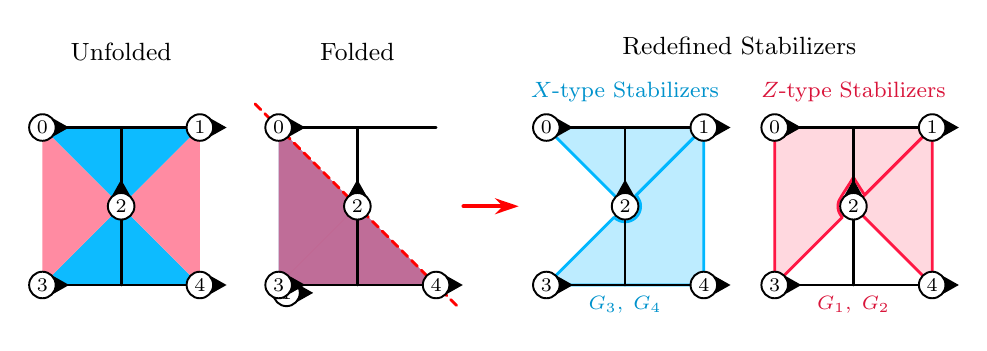
\begin{tikzpicture}[line cap=round,line join=round,thick,scale=1.0]
  \coordinate (Left)   at (-4.85, 0);
  \coordinate (Middle) at (-1.85, 0);
  \coordinate (XGrid)  at ( 1.55, 0);
  \coordinate (ZGrid)  at ( 4.45, 0);

  \node[above,font=\small] at ($(Left)+(0,1.72)$) {Unfolded};
  \node[above,font=\small] at ($(Middle)+(0,1.72)$) {Folded};
  \node[above,font=\small] at ($(XGrid)!0.5!(ZGrid)+(0,1.80)$) {Redefined Stabilizers};
  \node[above,font=\footnotesize,text=Xcol!80!black] at ($(XGrid)+(0,1.20)$) {$X$-type Stabilizers};
  \node[above,font=\footnotesize,text=Zcol!85!black] at ($(ZGrid)+(0,1.20)$) {$Z$-type Stabilizers};
  \node[font=\scriptsize,text=Xcol!80!black] at ($(XGrid)+(0,-1.25)$) {$G_3,\;G_4$};
  \node[font=\scriptsize,text=Zcol!85!black] at ($(ZGrid)+(0,-1.25)$) {$G_1,\;G_2$};

  % --- Left Patch (Unfolded) ---
  \begin{scope}[shift={(Left)}]
    \FiveQPatchFilled
    \FiveQPatchCircles
  \end{scope}

  % --- Middle Patch (Folded) ---
  \begin{scope}[shift={(Middle)}]
    \FiveQPatchOverlapped
    \def\m{0.30}
    \draw[dashed, draw=red, line width=1pt, dash pattern=on 3pt off 2pt]
      ($(q0)+(-\m,\m)$) -- ($(q4)+(\m,-\m)$);
    \FiveQPatchCirclesOneUnderThree
  \end{scope}

  \draw[-{Stealth[length=3mm,width=2mm]},red,line width=1.6pt]
    ($(Middle)+(1.35,0)$) -- ($(XGrid)+(-1.35,0)$);

  % --- Redefined X-type grid ---
  \begin{scope}[shift={(XGrid)}]
    \FiveQPatchRedefinedXGrid
    \FiveQPatchCircles
  \end{scope}

  % --- Redefined Z-type grid ---
  \begin{scope}[shift={(ZGrid)}]
    \FiveQPatchRedefinedZGrid
    \FiveQPatchCircles
  \end{scope}
\end{tikzpicture}
\caption{5-Qutrit Surface Code Patch}
\end{subfigure}

\vspace{2.0ex}

% ===================== (b) Definition =====================
\hspace*{-1.5em}
\begin{subfigure}[c]{0.48\textwidth}
\centering
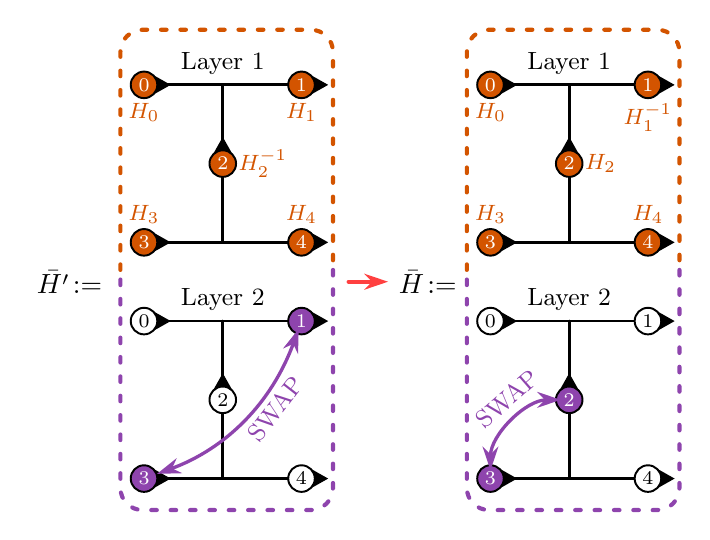
\begin{tikzpicture}[line cap=round,line join=round,thick,scale=1.0]
  \coordinate (LeftTop) at (-2.2,  1.50);
  \coordinate (LeftBot) at (-2.2, -1.50);
  \coordinate (RightTop) at ( 2.2,  1.50);
  \coordinate (RightBot) at ( 2.2, -1.50);

  \node[scale=1.0, anchor=east] at ($(LeftTop)+(-1.4, -1.5)$) {$\bar{H'}\!:=$};
  \node[scale=1.0, anchor=east] (HLabel) at ($(RightTop)+(-1.3, -1.5)$) {$\bar{H}\!:=$};

  \def\lw{1.5pt} \def\rc{8pt}
  % LEFT BOX 
  \path let \p1 = ($(LeftTop)+(-1.3,1.7)$), \p2 = ($(LeftBot)+(1.4,-1.4)$)
        in coordinate (LTL) at (\x1,\y1) coordinate (LBR) at (\x2,\y2)
           coordinate (LTR) at (\x2,\y1) coordinate (LBL) at (\x1,\y2);
  \coordinate (LMidLeft) at ($(LTL)!0.5!(LBL)$); \coordinate (LMidRight) at ($(LTR)!0.5!(LBR)$);
  \draw[HCol, dash pattern=on 2pt off 5pt, line width=\lw, rounded corners=\rc] (LMidLeft)--(LTL)--(LTR)--(LMidRight);
  \draw[SwapCol, dash pattern=on 2pt off 5pt, line width=\lw, rounded corners=\rc] (LMidRight)--(LBR)--(LBL)--(LMidLeft);

  % RIGHT BOX
  \path let \p1 = ($(RightTop)+(-1.3,1.7)$), \p2 = ($(RightBot)+(1.4,-1.4)$)
        in coordinate (RTL) at (\x1,\y1) coordinate (RBR) at (\x2,\y2)
           coordinate (RTR) at (\x2,\y1) coordinate (RBL) at (\x1,\y2);
  \coordinate (RMidLeft) at ($(RTL)!0.5!(RBL)$); \coordinate (RMidRight) at ($(RTR)!0.5!(RBR)$);
  \draw[HCol, dash pattern=on 2pt off 5pt, line width=\lw, rounded corners=\rc] (RMidLeft)--(RTL)--(RTR)--(RMidRight);
  \draw[SwapCol, dash pattern=on 2pt off 5pt, line width=\lw, rounded corners=\rc] (RMidRight)--(RBR)--(RBL)--(RMidLeft);

  \begin{scope}[shift={(LeftTop)}]
    \FiveQPatchEdges
    \foreach \P/\txt in {q0/0,q1/1,q2/2,q3/3,q4/4}{ \draw[line width=\qdLine,fill=HCol] (\P) circle (\qdR); \node[font=\numFont, text=white] at (\P) {\txt}; }
    \WedgeArrow{q0}{0}\WedgeArrow{q1}{0}\WedgeArrow{q3}{0}\WedgeArrow{q4}{0}\WedgeArrow{q2}{90}
    \node[anchor=south, font=\small, yshift=0mm] at (0, 1.0) {Layer 1};
    \begin{scope}[text=HCol, font=\footnotesize]
       \node[below, yshift=-3pt] at (q0) {$H_0$}; \node[below, yshift=-3pt] at (q1) {$H_1$};
       \node[right, xshift=2pt]  at (q2) {$H_2^{-1}$}; \node[above, yshift=3pt]  at (q3) {$H_3$}; \node[above, yshift=3pt]  at (q4) {$H_4$};
    \end{scope}
  \end{scope}

  \begin{scope}[shift={(LeftBot)}]
    \FiveQPatchEdges
    \foreach \P/\txt in {q0/0,q2/2,q4/4}{ \draw[line width=\qdLine,fill=white] (\P) circle (\qdR); \node[font=\numFont] at (\P) {\txt}; }
    \foreach \P/\txt in {q1/1,q3/3}{ \draw[line width=\qdLine,fill=SwapCol] (\P) circle (\qdR); \node[font=\numFont, text=white] at (\P) {\txt}; }
    \WedgeArrow{q0}{0}\WedgeArrow{q1}{0}\WedgeArrow{q3}{0}\WedgeArrow{q4}{0}\WedgeArrow{q2}{90}
    \node[anchor=south, font=\small, yshift=0mm] at (0, 1.0) {Layer 2};
    \draw[{Stealth[length=3mm,width=2mm]}-{Stealth[length=3mm,width=2mm]}, color=SwapCol, line width=1.2pt, shorten >=5pt, shorten <=3pt]
      (q1) to[bend left=25] node[midway, below right, rotate=52, xshift=-7pt, font=\small] {SWAP} (q3);
  \end{scope}

  \draw[-{Stealth[length=3mm,width=2mm]},red!75,line width=1.6pt] (-0.6, 0) -- (-0.1, 0);

  \begin{scope}[shift={(RightTop)}]
    \FiveQPatchEdges
    \foreach \P/\txt in {q0/0,q1/1,q2/2,q3/3,q4/4}{ \draw[line width=\qdLine,fill=HCol] (\P) circle (\qdR); \node[font=\numFont, text=white] at (\P) {\txt}; }
    \WedgeArrow{q0}{0}\WedgeArrow{q1}{0}\WedgeArrow{q3}{0}\WedgeArrow{q4}{0}\WedgeArrow{q2}{90}
    \node[anchor=south, font=\small, yshift=0mm] at (0, 1.0) {Layer 1};
    \begin{scope}[text=HCol, font=\footnotesize]
       \node[below, yshift=-3pt] at (q0) {$H_0$}; \node[below, yshift=-3pt] at (q1) {$H_1^{-1}$};
       \node[right, xshift=2pt]  at (q2) {$H_2$}; \node[above, yshift=3pt]  at (q3) {$H_3$}; \node[above, yshift=3pt]  at (q4) {$H_4$};
    \end{scope}
  \end{scope}

  \begin{scope}[shift={(RightBot)}]
    \FiveQPatchEdges
    \foreach \P/\txt in {q0/0,q1/1,q4/4}{ \draw[line width=\qdLine,fill=white] (\P) circle (\qdR); \node[font=\numFont] at (\P) {\txt}; }
    \foreach \P/\txt in {q2/2,q3/3}{ \draw[line width=\qdLine,fill=SwapCol] (\P) circle (\qdR); \node[font=\numFont, text=white] at (\P) {\txt}; }
    \WedgeArrow{q0}{0}\WedgeArrow{q1}{0}\WedgeArrow{q3}{0}\WedgeArrow{q4}{0}\WedgeArrow{q2}{90}
    \node[anchor=south, font=\small, yshift=0mm] at (0, 1.0) {Layer 2};
    \draw[{Stealth[length=3mm,width=2mm]}-{Stealth[length=3mm,width=2mm]}, color=SwapCol, line width=1.2pt, shorten >=3pt, shorten <=3pt]
      (q2) to[bend right=45] node[midway, below, xshift =-7pt, yshift=14pt, rotate=41, font=\small] {SWAP} (q3);
  \end{scope}
\end{tikzpicture}
\caption{Logical $H$}
\label{fig: logical H}
\end{subfigure}
\quad
% ===================== (c) S Definition =====================
\begin{subfigure}[c]{0.48\textwidth}
\centering
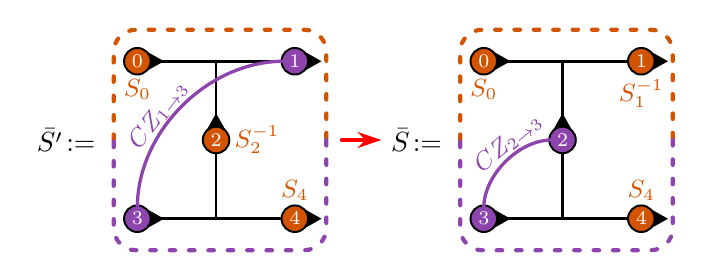
\begin{tikzpicture}[line cap=round,line join=round,thick,scale=1.0]
  \coordinate (Left)  at (-2.2, 0);
  \coordinate (Right) at ( 2.2, 0);
  \def\lw{1.5pt} \def\rc{8pt}

  \coordinate (LTL) at ($(Left)+(-1.3, 1.4)$); \coordinate (LBR) at ($(Left)+(1.4, -1.4)$);
  \coordinate (LTR) at ($(Left)+(1.4, 1.4)$);  \coordinate (LBL) at ($(Left)+(-1.3, -1.4)$);
  \coordinate (LMidLeft) at ($(LTL)!0.5!(LBL)$); \coordinate (LMidRight) at ($(LTR)!0.5!(LBR)$);
  \draw[HCol, dash pattern=on 2pt off 5pt, line width=\lw, rounded corners=\rc] (LMidLeft)--(LTL)--(LTR)--(LMidRight);
  \draw[SwapCol, dash pattern=on 2pt off 5pt, line width=\lw, rounded corners=\rc] (LMidRight)--(LBR)--(LBL)--(LMidLeft);

  \coordinate (RTL) at ($(Right)+(-1.3, 1.4)$); \coordinate (RBR) at ($(Right)+(1.4, -1.4)$);
  \coordinate (RTR) at ($(Right)+(1.4, 1.4)$);  \coordinate (RBL) at ($(Right)+(-1.3, -1.4)$);
  \coordinate (RMidLeft) at ($(RTL)!0.5!(RBL)$); \coordinate (RMidRight) at ($(RTR)!0.5!(RBR)$);
  \draw[HCol, dash pattern=on 2pt off 5pt, line width=\lw, rounded corners=\rc] (RMidLeft)--(RTL)--(RTR)--(RMidRight);
  \draw[SwapCol, dash pattern=on 2pt off 5pt, line width=\lw, rounded corners=\rc] (RMidRight)--(RBR)--(RBL)--(RMidLeft);

  \node[scale=1.0, anchor=east] at ($(Left)+(-1.4, 0)$) {$\bar{S'}\!:=$};
  \node[scale=1.0, anchor=east] (SLabel) at ($(Right)+(-1.4, 0)$) {$\bar{S}\!:=$};

  \newcommand{\DrawLHSPattern}{
      \FiveQPatchEdges
      \foreach \P in {q0, q2, q4} { \draw[line width=\qdLine,fill=HCol] (\P) circle (\qdR); }
      \foreach \P in {q1, q3} { \draw[line width=\qdLine,fill=SwapCol] (\P) circle (\qdR); }
      \foreach \P/\txt in {q0/0,q1/1,q2/2,q3/3,q4/4}{ \node[font=\numFont, text=white] at (\P) {\txt}; }
      \WedgeArrow{q0}{0}\WedgeArrow{q1}{0}\WedgeArrow{q3}{0}\WedgeArrow{q4}{0}\WedgeArrow{q2}{90}
      \node[text=HCol, font=\small, below, yshift=-3pt] at (q0) {$S_0$};
      \node[text=HCol, font=\small, right, xshift=3pt] at (q2) {$S_2^{-1}$};
      \node[text=HCol, font=\small, above, yshift=3pt] at (q4) {$S_4$};
      \draw[color=SwapCol, line width=1.2pt, shorten <=4pt, shorten >=4pt] 
         (q1) to[out=180, in=90] coordinate[pos=0.45] (mid) (q3);
      \node[text=SwapCol, font=\small, rotate=52, anchor=south, xshift=-12pt, yshift=-1pt] at (mid) {$CZ_{1\to 3}$};
  }
  \newcommand{\DrawRHSPattern}{
      \FiveQPatchEdges
      \foreach \P in {q0, q1, q4} { \draw[line width=\qdLine,fill=HCol] (\P) circle (\qdR); }
      \foreach \P in {q2, q3} { \draw[line width=\qdLine,fill=SwapCol] (\P) circle (\qdR); }
      \foreach \P/\txt in {q0/0,q1/1,q2/2,q3/3,q4/4}{ \node[font=\numFont, text=white] at (\P) {\txt}; }
      \WedgeArrow{q0}{0}\WedgeArrow{q1}{0}\WedgeArrow{q3}{0}\WedgeArrow{q4}{0}\WedgeArrow{q2}{90}
      \node[text=HCol, font=\small, below, yshift=-3pt] at (q0) {$S_0$};
      \node[text=HCol, font=\small, below, yshift=-3pt] at (q1) {$S_1^{-1}$};
      \node[text=HCol, font=\small, above, yshift=3pt] at (q4) {$S_4$};
      \draw[color=SwapCol, line width=1.2pt, shorten <=4pt, shorten >=4pt] 
         (q3) to[out=90, in=180] coordinate[pos=0.5] (midR) (q2);
      \node[text=SwapCol, font=\small, rotate=40, anchor=south, xshift=5pt, yshift=-2pt] at (midR) {$CZ_{2\to 3}$};
  }
  \begin{scope}[shift={(Left)}] \DrawLHSPattern \end{scope}
  \begin{scope}[shift={(Right)}] \DrawRHSPattern \end{scope}
  \draw[-{Stealth[length=3mm,width=2mm]},red,line width=1.6pt] (-0.6, 0) -- (-0.1, 0);
\end{tikzpicture}
\caption{Logical $S$}
\label{fig: logical S}
\end{subfigure}

\vspace{2.0ex}

% ===================== (d) Parallel Operations =====================
\begin{subfigure}[b]{0.9\textwidth}
\centering
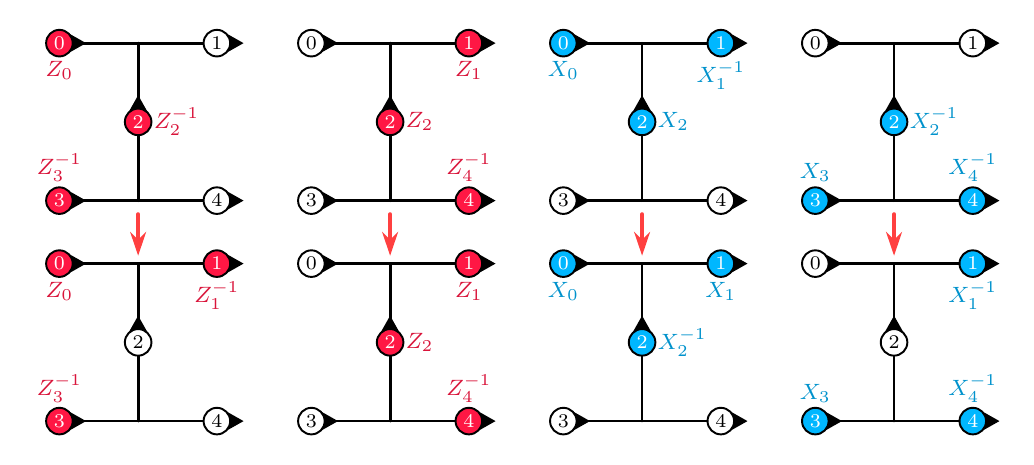
\begin{tikzpicture}[line cap=round,line join=round,thick,scale=1.0]
  \def\yTop{1.6} \def\yBot{-1.2}

  % COL 1
  \def\x{-4.8}
  \begin{scope}[shift={(\x, \yTop)}]
     \FiveQPatchEdges
     \foreach \P/\txt in {q1/1, q4/4}{ \draw[line width=\qdLine,fill=white] (\P) circle (\qdR); \node[font=\numFont] at (\P) {\txt}; }
     \foreach \P/\txt in {q0/0, q2/2, q3/3}{ \draw[line width=\qdLine,fill=Zcol] (\P) circle (\qdR); \node[font=\numFont, text=white] at (\P) {\txt}; }
     \WedgeArrow{q0}{0}\WedgeArrow{q1}{0}\WedgeArrow{q3}{0}\WedgeArrow{q4}{0}\WedgeArrow{q2}{90}
     \begin{scope}[text=Zcol!85!black, font=\footnotesize]
        \node[below, yshift=-3pt] at (q0) {$Z_0$}; \node[right, xshift=2pt] at (q2) {$Z_2^{-1}$}; \node[above, yshift=3pt] at (q3) {$Z_3^{-1}$};
     \end{scope}
  \end{scope}
  \begin{scope}[shift={(\x, \yBot)}]
     \FiveQPatchEdges
     \foreach \P/\txt in {q2/2, q4/4}{ \draw[line width=\qdLine,fill=white] (\P) circle (\qdR); \node[font=\numFont] at (\P) {\txt}; }
     \foreach \P/\txt in {q0/0, q1/1, q3/3}{ \draw[line width=\qdLine,fill=Zcol] (\P) circle (\qdR); \node[font=\numFont, text=white] at (\P) {\txt}; }
     \WedgeArrow{q0}{0}\WedgeArrow{q1}{0}\WedgeArrow{q3}{0}\WedgeArrow{q4}{0}\WedgeArrow{q2}{90}
     \begin{scope}[text=Zcol!85!black, font=\footnotesize]
        \node[below, yshift=-3pt] at (q0) {$Z_0$}; \node[below, yshift=-3pt] at (q1) {$Z_1^{-1}$}; \node[above, yshift=3pt] at (q3) {$Z_3^{-1}$};
     \end{scope}
  \end{scope}
  \draw[-{Stealth[length=3mm,width=2mm]},red!75,line width=1.6pt] (\x, 0.425) -- (\x, -0.1);

  % COL 2
  \def\x{-1.6}
  \begin{scope}[shift={(\x, \yTop)}]
     \FiveQPatchEdges
     \foreach \P/\txt in {q0/0, q3/3}{ \draw[line width=\qdLine,fill=white] (\P) circle (\qdR); \node[font=\numFont] at (\P) {\txt}; }
     \foreach \P/\txt in {q1/1, q2/2, q4/4}{ \draw[line width=\qdLine,fill=Zcol] (\P) circle (\qdR); \node[font=\numFont, text=white] at (\P) {\txt}; }
     \WedgeArrow{q0}{0}\WedgeArrow{q1}{0}\WedgeArrow{q3}{0}\WedgeArrow{q4}{0}\WedgeArrow{q2}{90}
     \begin{scope}[text=Zcol!85!black, font=\footnotesize]
        \node[below, yshift=-3pt] at (q1) {$Z_1$}; \node[right, xshift=2pt] at (q2) {$Z_2$}; \node[above, yshift=3pt] at (q4) {$Z_4^{-1}$};
     \end{scope}
  \end{scope}
  \begin{scope}[shift={(\x, \yBot)}]
     \FiveQPatchEdges
     \foreach \P/\txt in {q0/0, q3/3}{ \draw[line width=\qdLine,fill=white] (\P) circle (\qdR); \node[font=\numFont] at (\P) {\txt}; }
     \foreach \P/\txt in {q1/1, q2/2, q4/4}{ \draw[line width=\qdLine,fill=Zcol] (\P) circle (\qdR); \node[font=\numFont, text=white] at (\P) {\txt}; }
     \WedgeArrow{q0}{0}\WedgeArrow{q1}{0}\WedgeArrow{q3}{0}\WedgeArrow{q4}{0}\WedgeArrow{q2}{90}
     \begin{scope}[text=Zcol!85!black, font=\footnotesize]
        \node[below, yshift=-3pt] at (q1) {$Z_1$}; \node[right, xshift=2pt] at (q2) {$Z_2$}; \node[above, yshift=3pt] at (q4) {$Z_4^{-1}$};
     \end{scope}
  \end{scope}
  \draw[-{Stealth[length=3mm,width=2mm]},red!75,line width=1.6pt] (\x, 0.425) -- (\x, -0.1);

  % COL 3
  \def\x{1.6}
  \begin{scope}[shift={(\x, \yTop)}]
     \FiveQPatchEdges
     \foreach \P/\txt in {q3/3, q4/4}{ \draw[line width=\qdLine,fill=white] (\P) circle (\qdR); \node[font=\numFont] at (\P) {\txt}; }
     \foreach \P/\txt in {q0/0, q1/1, q2/2}{ \draw[line width=\qdLine,fill=Xcol] (\P) circle (\qdR); \node[font=\numFont, text=white] at (\P) {\txt}; }
     \WedgeArrow{q0}{0}\WedgeArrow{q1}{0}\WedgeArrow{q3}{0}\WedgeArrow{q4}{0}\WedgeArrow{q2}{90}
     \begin{scope}[text=Xcol!80!black, font=\footnotesize]
        \node[below, yshift=-3pt] at (q0) {$X_0$}; \node[below, yshift=-3pt] at (q1) {$X_1^{-1}$}; \node[right, xshift=2pt] at (q2) {$X_2$};
     \end{scope}
  \end{scope}
  \begin{scope}[shift={(\x, \yBot)}]
     \FiveQPatchEdges
     \foreach \P/\txt in {q3/3, q4/4}{ \draw[line width=\qdLine,fill=white] (\P) circle (\qdR); \node[font=\numFont] at (\P) {\txt}; }
     \foreach \P/\txt in {q0/0, q1/1, q2/2}{ \draw[line width=\qdLine,fill=Xcol] (\P) circle (\qdR); \node[font=\numFont, text=white] at (\P) {\txt}; }
     \WedgeArrow{q0}{0}\WedgeArrow{q1}{0}\WedgeArrow{q3}{0}\WedgeArrow{q4}{0}\WedgeArrow{q2}{90}
     \begin{scope}[text=Xcol!80!black, font=\footnotesize]
        \node[below, yshift=-3pt] at (q0) {$X_0$}; \node[below, yshift=-3pt] at (q1) {$X_1$}; \node[right, xshift=2pt] at (q2) {$X_2^{-1}$};
     \end{scope}
  \end{scope}
  \draw[-{Stealth[length=3mm,width=2mm]},red!75,line width=1.6pt] (\x, 0.425) -- (\x, -0.1);

  % COL 4
  \def\x{4.8}
  \begin{scope}[shift={(\x, \yTop)}]
     \FiveQPatchEdges
     \foreach \P/\txt in {q0/0, q1/1}{ \draw[line width=\qdLine,fill=white] (\P) circle (\qdR); \node[font=\numFont] at (\P) {\txt}; }
     \foreach \P/\txt in {q2/2, q3/3, q4/4}{ \draw[line width=\qdLine,fill=Xcol] (\P) circle (\qdR); \node[font=\numFont, text=white] at (\P) {\txt}; }
     \WedgeArrow{q0}{0}\WedgeArrow{q1}{0}\WedgeArrow{q3}{0}\WedgeArrow{q4}{0}\WedgeArrow{q2}{90}
     \begin{scope}[text=Xcol!80!black, font=\footnotesize]
        \node[right, xshift=2pt] at (q2) {$X_2^{-1}$}; \node[above, yshift=3pt] at (q3) {$X_3$}; \node[above, yshift=3pt] at (q4) {$X_4^{-1}$};
     \end{scope}
  \end{scope}
  \begin{scope}[shift={(\x, \yBot)}]
     \FiveQPatchEdges
     \foreach \P/\txt in {q0/0, q2/2}{ \draw[line width=\qdLine,fill=white] (\P) circle (\qdR); \node[font=\numFont] at (\P) {\txt}; }
     \foreach \P/\txt in {q1/1, q3/3, q4/4}{ \draw[line width=\qdLine,fill=Xcol] (\P) circle (\qdR); \node[font=\numFont, text=white] at (\P) {\txt}; }
     \WedgeArrow{q0}{0}\WedgeArrow{q1}{0}\WedgeArrow{q3}{0}\WedgeArrow{q4}{0}\WedgeArrow{q2}{90}
     \begin{scope}[text=Xcol!80!black, font=\footnotesize]
        \node[below, yshift=-3pt] at (q1) {$X_1^{-1}$}; \node[above, yshift=3pt] at (q3) {$X_3$}; \node[above, yshift=3pt] at (q4) {$X_4^{-1}$};
     \end{scope}
  \end{scope}
  \draw[-{Stealth[length=3mm,width=2mm]},red!75,line width=1.6pt] (\x, 0.425) -- (\x, -0.1);
\end{tikzpicture}
\caption{Stabilizers for the $[[5,1,2]]_3$ code}
\end{subfigure}

\vspace{2.0ex}
% ===================== (e) Logical X =====================
\begin{subfigure}[c]{0.35\textwidth}
\centering
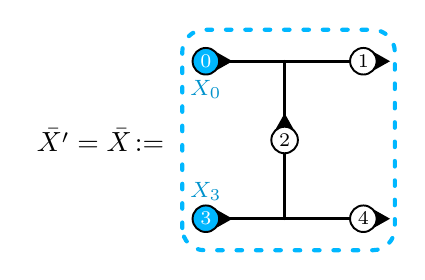
\begin{tikzpicture}[line cap=round,line join=round,thick,scale=1.0]
  \node[scale=1.0, anchor=east] at (-1.4, 0) {$\bar{X'}=\bar{X}\!:=$};
   
  % Added blue box
  \def\lw{1.5pt} \def\rc{8pt}
  \coordinate (LTL_X) at (-1.3, 1.4); \coordinate (LBR_X) at (1.4, -1.4);
  \coordinate (LTR_X) at ( 1.4, 1.4); \coordinate (LBL_X) at (-1.3, -1.4);
  \draw[Xcol, dash pattern=on 2pt off 5pt, line width=\lw, rounded corners=\rc] (LBL_X)--(LTL_X)--(LTR_X)--(LBR_X)--cycle;
   
  \FiveQPatchEdges
  \foreach \P/\txt in {q1/1, q2/2, q4/4}{ \draw[line width=\qdLine,fill=white] (\P) circle (\qdR); \node[font=\numFont] at (\P) {\txt}; }
  \foreach \P/\txt in {q0/0, q3/3}{ \draw[line width=\qdLine,fill=Xcol] (\P) circle (\qdR); \node[font=\numFont, text=white] at (\P) {\txt}; }
  \WedgeArrow{q0}{0}\WedgeArrow{q1}{0}\WedgeArrow{q3}{0}\WedgeArrow{q4}{0}\WedgeArrow{q2}{90}
  \begin{scope}[text=Xcol!80!black, font=\footnotesize]
     \node[below, yshift=-3pt] at (q0) {$X_0$};
     \node[above, yshift=3pt]  at (q3) {$X_3$};
  \end{scope}
\end{tikzpicture}
\caption{Logical $X$}
\end{subfigure}
\quad
% ===================== (f) Logical Z =====================
\begin{subfigure}[c]{0.6\textwidth}
\centering
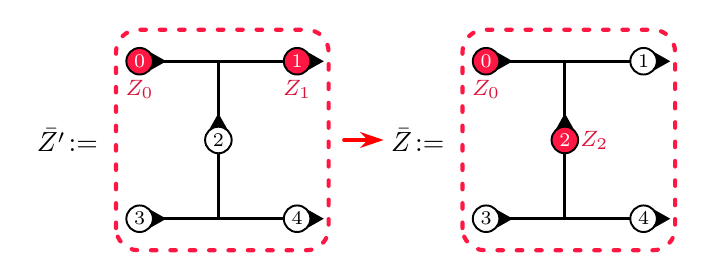
\begin{tikzpicture}[line cap=round,line join=round,thick,scale=1.0]
  % Define centers
  \coordinate (Left)  at (-2.2, 0);
  \coordinate (Right) at ( 2.2, 0);

  % Labels
  \node[scale=1.0, anchor=east] at ($(Left)+(-1.4, 0)$) {$\bar{Z'}\!:=$};
  \node[scale=1.0, anchor=east] at ($(Right)+(-1.4, 0)$) {$\bar{Z}\!:=$};
   
  % Added red boxes
  \def\lw{1.5pt} \def\rc{8pt}
  % Left Box
  \coordinate (LTL_Z) at ($(Left)+(-1.3, 1.4)$); \coordinate (LBR_Z) at ($(Left)+(1.4, -1.4)$);
  \coordinate (LTR_Z) at ($(Left)+(1.4, 1.4)$); \coordinate (LBL_Z) at ($(Left)+(-1.3, -1.4)$);
  \draw[Zcol, dash pattern=on 2pt off 5pt, line width=\lw, rounded corners=\rc] (LBL_Z)--(LTL_Z)--(LTR_Z)--(LBR_Z)--cycle;

  % Right Box
  \coordinate (RTL_Z) at ($(Right)+(-1.3, 1.4)$); \coordinate (RBR_Z) at ($(Right)+(1.4, -1.4)$);
  \coordinate (RTR_Z) at ($(Right)+(1.4, 1.4)$); \coordinate (RBL_Z) at ($(Right)+(-1.3, -1.4)$);
  \draw[Zcol, dash pattern=on 2pt off 5pt, line width=\lw, rounded corners=\rc] (RBL_Z)--(RTL_Z)--(RTR_Z)--(RBR_Z)--cycle;

  % Left Patch: Z0 Z1
  \begin{scope}[shift={(Left)}]
     \FiveQPatchEdges
     \foreach \P/\txt in {q2/2, q3/3, q4/4}{ \draw[line width=\qdLine,fill=white] (\P) circle (\qdR); \node[font=\numFont] at (\P) {\txt}; }
     \foreach \P/\txt in {q0/0, q1/1}{ \draw[line width=\qdLine,fill=Zcol] (\P) circle (\qdR); \node[font=\numFont, text=white] at (\P) {\txt}; }
     \WedgeArrow{q0}{0}\WedgeArrow{q1}{0}\WedgeArrow{q3}{0}\WedgeArrow{q4}{0}\WedgeArrow{q2}{90}
     \begin{scope}[text=Zcol!85!black, font=\footnotesize]
        \node[below, yshift=-3pt] at (q0) {$Z_0$};
        \node[below, yshift=-3pt] at (q1) {$Z_1$};
     \end{scope}
  \end{scope}

  % Right Patch: Z0 Z2
  \begin{scope}[shift={(Right)}]
     \FiveQPatchEdges
     \foreach \P/\txt in {q1/1, q3/3, q4/4}{ \draw[line width=\qdLine,fill=white] (\P) circle (\qdR); \node[font=\numFont] at (\P) {\txt}; }
     \foreach \P/\txt in {q0/0, q2/2}{ \draw[line width=\qdLine,fill=Zcol] (\P) circle (\qdR); \node[font=\numFont, text=white] at (\P) {\txt}; }
     \WedgeArrow{q0}{0}\WedgeArrow{q1}{0}\WedgeArrow{q3}{0}\WedgeArrow{q4}{0}\WedgeArrow{q2}{90}
     \begin{scope}[text=Zcol!85!black, font=\footnotesize]
        \node[below, yshift=-3pt] at (q0) {$Z_0$};
        \node[right, xshift=2pt]  at (q2) {$Z_2$};
     \end{scope}
  \end{scope}

  % Arrow in middle (adjusted for gap)
  \draw[-{Stealth[length=3mm,width=2mm]},red,line width=1.6pt] (-0.6, 0) -- (-0.1, 0);

\end{tikzpicture}
\caption{Logical $Z$}
\end{subfigure}
% END OF PAGE 1
\end{figure}

\begin{figure}[H]\ContinuedFloat
\centering
% ===== MAIN CAPTION HERE =====
\caption{Comparison of 5-qutrit surface code definitions and logical operators. 
(a) The left-hand side (LHS) shows the conventional folded and unfolded definitions from \cite{Moussa2016}. Blue and red regions represent truncated conventional $X$- and $Z$-type stabilizers, respectively. In the folded version, blended colors indicate the mirror duality between these stabilizers. The right-hand side (RHS) illustrates the proposed convention, with the redefined $X$- and $Z$-type stabilizers shown on separate grids using colored patch perimeters. This avoids the folding procedure via local SWAPs, thereby eliminating the need for additional ancillas. 
(b) The proposed logical Hadamard gate, $\bar{H}$. Together with the logical Phase gate $\bar{S}$ shown in (c), these operators generate the single-qutrit logical Clifford group. Unlike the conventional $\bar{H'}$, this implementation requires only nearest-neighbor SWAP gates in Layer 2. 
(c) The proposed logical Phase gate, $\bar{S}$, which utilizes only nearest-neighbor $CZ$ gates, distinct from the conventional $\bar{S'}$. 
(d) Redefined $X$- and $Z$-type stabilizers, selected to be preserved by the logical Clifford group while maintaining mirror dual symmetry. 
(e) The logical $\bar{X}$ operator (unchanged). 
(f) The redefined logical $\bar{Z}$, constructed to commute with stabilizers and generate the Pauli group with $\bar{X}$, ensuring the Pauli group is preserved by the logical Clifford group.}
\label{fig: 5-qutrit-code}

\end{figure}



\subsubsection{Encoding Circuit}

To initialize the system in the code space, we employ a specific unitary circuit that maps the physical ground state $\ket{0}^{\otimes 5}$ to the logical state $\ket{\bar{+}}$. This state corresponds to the $+1$ eigenstate of the logical Pauli operator $\overline{X} = X_0 \otimes X_3$, defined in Eq.~\eqref{eq:logicalPauli}.

\begin{figure}[htbp]
    \centering
    \begin{quantikz}
      \lstick{$q_0: \ket{0}$} & \qw & \qw & \gate{X_3} & \gate{X_3} & \qw \\
      \lstick{$q_1: \ket{0}$} & \qw & \gate{X_3^{\dagger}} & \ctrl{-1} & \qw & \qw \\
      \lstick{$q_2: \ket{0}$} & \gate{H_3^{\dagger}} & \ctrl{-1} & \gate{X_3} & \qw & \qw \\
      \lstick{$q_3: \ket{0}$} & \gate{H_3^{\dagger}} & \qw & \qw & \ctrl{-3}  & \qw \\
      \lstick{$q_4: \ket{0}$} & \gate{H_3^{\dagger}} & \qw & \ctrl{-2}  & \qw  & \qw
    \end{quantikz}
    \caption{Non-fault-tolerant encoding circuit for the $[[5,1,2]]_3$ surface code. The circuit maps the physical state $\ket{0}^{\otimes 5}$ to the logical state $\ket{\bar{+}}$, which is the $+1$ eigenstate of the logical $\bar{X}$ operator. The gates denoted are qutrit Hadamard ($H_3$) and Generalized SUM/CNOT gates. In our simulations this circuit is noiseless (\autoref{sub:noise_models}). On hardware, errors occurring during state preparation contribute SPAM errors to the LRB-D protocol.}
    \label{fig:encoding_circuit}
\end{figure}

The encoding circuit shown in \autoref{fig:encoding_circuit} is a non-fault-tolerant state preparation sequence that minimizes the use of ancillas and the physical gate count. In the simulations of this work the encoding is noiseless, so it contributes no error. On hardware, the quality of the encoding step is classified under State Preparation and Measurement (SPAM) errors. As established in standard RB theory, these SPAM errors are absorbed into the $A$ and $B$ parameters of the fidelity decay curve (Eq.~\eqref{eq:fseq}) and do not affect the extracted decay parameter $f$ or the estimated gate fidelity \cite{Magesan2011PRL,Magesan2012PRA}. With the offset fixed to $B = 0$ (\autoref{sub:fit_model}), they enter through $A$ alone. Consequently, a compact, non-fault-tolerant encoding is sufficient for providing a consistent entry point into the logical code space for benchmarking purposes.


\subsection{Logical Randomized Benchmarking with Detection (LRB-D)}
\label{sub:lrb_d}

Standard Logical Randomized Benchmarking (LRB) characterizes the performance of a code by actively correcting errors using decoder feedback throughout the Clifford sequence \cite{Combes2017}. However, the $[[5,1,2]]_3$ code used in this work has distance $d=2$. It can detect the presence of any single-qutrit error, but it cannot identify the location and type of the error without ambiguity. Consequently, the code violates the Knill-Laflamme error correction conditions for generic single-qutrit errors, and faithful error correction is impossible.

We therefore use a detection-only variant of the protocol, denoted LRB-D. Instead of attempting to correct errors and return the system to the code space, LRB-D treats the stabilizer measurements as a filter. We keep only the shots in which every checked syndrome is trivial and discard every shot (experimental run) in which a non-trivial syndrome is detected. LRB-D thus benchmarks how well the code preserves the logical information in the absence of detectable errors.

We first simulate the protocol with the \texttt{sdim} qudit stabilizer simulator under the circuit-level noise models of \autoref{sub:noise_models}, before running it on the IQM Garnet QPU. The simulations test the expected logical fidelity decay and the effect of the postselection filter under controlled noise.

\subsubsection{LRB-D Protocol}
An LRB-D circuit of depth $m$ consists of the following steps, illustrated in \autoref{fig:lrb_d_full}:

\begin{enumerate}
    \item \textbf{Logical State Preparation:} The encoding circuit of \autoref{fig:encoding_circuit} prepares the logical state $\ket{\bar{+}}$, the $+1$ eigenstate of the logical $\bar{X}$ operator.

    \item \textbf{Random Logical Clifford Sequence with Checks:} We draw $m$ logical Cliffords $\bar C_1, \dots, \bar C_m$ independently and uniformly from the $216$-element single-qutrit Clifford group (\autoref{sec:clifford-gen}) and apply them to the encoded state. Each $\bar C_j$ is a word in the transversal gates $\bar H$, $\bar S$, $\bar X$ and $\bar Z$ of \autoref{sec: error detection code}. A full stabilizer check round follows every forward Clifford. A check round resets all ancillas to $\ket{0}$, runs the syndrome extraction circuits of $G_1, \dots, G_4$ (\autoref{fig:lrb_c} and \autoref{fig:lrb_d}, or \autoref{fig:two_ancilla_checks} for the two-ancilla layout of \autoref{sub:ancilla_layouts}), and reads out all ancillas in its final moment. We call the check round after $\bar C_t$ round $t$.

    \textit{Simulation: Every logical Clifford and every check round is a separate segment of the circuit-level noise model (\autoref{sub:noise_models}). Every gate, reset, ancilla readout and idle location inside these segments carries the noise of \autoref{tab:circuit-noise}. The identity element is applied as an identity gate that occupies one idle moment.}

    \item \textbf{Mirror Inverse:} We then apply the inverses in reverse order, $\bar C_m^{-1}, \bar C_{m-1}^{-1}, \dots, \bar C_1^{-1}$. The inverse of each element is looked up in the Clifford catalog and applied as an ordinary logical Clifford. No check round separates consecutive inverses. In the absence of errors the mirror inverse returns the system to $\ket{\bar{+}}$.

    \textit{Simulation: Each inverse is a noisy segment like any forward Clifford, so a circuit of depth $m$ contains $2m$ noisy logical Cliffords. We never synthesize a single recovery gate $(\bar C_m \cdots \bar C_1)^{-1}$.}

    \item \textbf{Final Check Round:} One more check round, round $m+1$, follows the last inverse. A circuit of depth $m$ therefore contains $m+1$ check rounds.

    \item \textbf{Postselection:} A postselection schedule (\autoref{subsub:postselection}) selects a set $\mathcal{T}$ of rounds. We keep a shot only if every stabilizer outcome in every selected round is trivial:
    \begin{equation}
        \text{Keep shot if: } \forall\, t \in \mathcal{T},\ \forall\, j \in \{1, \dots, 4\}, \quad \text{outcome}_t(G_j) = 0 \pmod 3 .
    \end{equation}
    Any shot yielding a non-trivial syndrome in a selected round (eigenvalue $\omega$ or $\omega^2$, integer outcome 1 or 2) is discarded. In the two-ancilla layout the relay readouts of the selected rounds must also be $0$. Rounds outside $\mathcal{T}$ are still executed, and in simulation they still inject noise, but their outcomes are ignored. Terminal postselection uses separate circuits without check rounds and checks the final data readout instead (\autoref{subsub:postselection}).

    \item \textbf{Logical Measurement:} For the surviving shots, we read out the logical qutrit by measuring $q_0$ and $q_3$ in the $X$ basis, since $\bar{X} = X_0 \otimes X_3$. We obtain outcomes $x_0, x_3 \in \{0, 1, 2\}$, and the logical outcome is their modular sum,
    \begin{equation}
        x_{\bar{X}} = (x_0 + x_3) \pmod 3 .
    \end{equation}
    Each $X$-basis readout is $H^{-1}$ followed by a computational-basis measurement, so its outcome $j$ belongs to the $X$ eigenvalue $\omega^{-j}$. The result $x_{\bar{X}}=0$ therefore corresponds to the target eigenvalue $+1$, and the expectation value of the logical measurement is
    \begin{equation}
        \langle \bar{X} \rangle = P_0 + \omega^{2} P_1 + \omega P_2,
    \end{equation}
    where $P_j$ is the proportion of postselected shots yielding the logical outcome $j$. We compute the modulus $|\langle \bar{X} \rangle|$ for each random sequence and average it over the sequences. It equals $|P_0 + \omega P_1 + \omega^2 P_2|$, and this sequence average is the quantity that we fit.

    \textit{Simulation: The logical readout is noiseless.}
\end{enumerate}

\begin{figure}[H]
    \centering
    % --- Row 1: Part (a), the full protocol ---
    \begin{subfigure}[b]{\textwidth}
        \centering
        \scalebox{0.8}{
        \begin{quantikz}[row sep=0.45cm, column sep=0.22cm]
          \lstick{data $\ket{0}^{\otimes 5}$} & \qwbundle{5} &
            \gate{\textcolor{LightBlue}{U_{\mathrm{enc}}}} &
            \gate{\textcolor{red}{\bar C_j}}\gategroup[2,steps=4,style={dashed,rounded corners,inner xsep=2pt},background,label style={label position=below,anchor=north,yshift=-0.2cm}]{$j = 1, \dots, m$} &
            \gate[2]{\textcolor{purple}{\mathcal{N}}} &
            \gate[2]{\mathcal{R}_j} &
            \gate[2]{\textcolor{purple}{\mathcal{N}}} &
            &
            \gate{\textcolor{red}{\bar C_j^{-1}}}\gategroup[2,steps=2,style={dashed,rounded corners,inner xsep=2pt},background,label style={label position=below,anchor=north,yshift=-0.2cm}]{$j = m, \dots, 1$} &
            \gate[2]{\textcolor{purple}{\mathcal{N}}} &
            &
            \gate[2]{\mathcal{R}_{m+1}} &
            \gate[2]{\textcolor{purple}{\mathcal{N}}} &
            \meter{} & \rstick{$x_{\bar X}$} \\
          \lstick{ancillas $\ket{0}^{\otimes n_a}$} & \qwbundle{n_a} & & & & & & & & & & & & &
        \end{quantikz}
        }
        \vspace{0.2cm}
        \caption{Simulated LRB-D circuit of depth $m$}
        \label{fig:lrb_a}
    \end{subfigure}

    \vspace{0.3cm}
    % --- Row 2: Parts (b) and (c) ---
    \begin{subfigure}[b]{0.26\textwidth}
        \centering
        \scalebox{0.7}{
        \begin{quantikz}[row sep={0.75cm,between origins}, column sep=0.25cm]
          \lstick{$q_0$} & \gate{S_3} & \gate{\textcolor{purple}{\mathcal{E}_1}} & \qw \\
          \lstick{$q_1$} & \gate{S_3^{-1}} & \gate{\textcolor{purple}{\mathcal{E}_1}} & \qw \\
          \lstick{$q_2$} & \ctrl{1} & \gate[2]{\textcolor{purple}{\mathcal{E}_2}} & \qw \\
          \lstick{$q_3$} & \gate{Z_3} & & \qw \\
          \lstick{$q_4$} & \gate{S_3} & \gate{\textcolor{purple}{\mathcal{E}_1}} & \qw \\
          \lstick{ancillas} & \qwbundle{n_a} & \gate{\textcolor{purple}{\mathcal{E}_{\mathrm{idle}}}} & \qw
        \end{quantikz}
        }
        \caption{Noise in one segment, $\bar S$}
        \label{fig:lrb_b}
    \end{subfigure}
    \hfill
    \begin{subfigure}[b]{0.72\textwidth}
        \centering
        % G1
        \scalebox{0.62}{
        \begin{quantikz}[row sep={0.62cm,between origins}, column sep=0.3cm]
          \lstick{$q_0$} & \ctrl{5} & \qw & \qw & \qw \\
          \lstick{$q_1$} & \qw & \ctrl{4} & \qw & \qw \\
          \lstick{$q_2$} & \qw & \qw & \qw & \qw \\
          \lstick{$q_3$} & \qw & \qw & \ctrl{2} & \qw \\
          \lstick{$q_4$} & \qw & \qw & \qw & \qw \\
          \lstick{$a_1: \ket{0}$} & \gate{X_3} & \gate{X_3^{\dagger}} & \gate{X_3^{\dagger}} & \meter{}
        \end{quantikz}
        }
        \hspace{0.6cm}
        % G2
        \scalebox{0.62}{
        \begin{quantikz}[row sep={0.62cm,between origins}, column sep=0.3cm]
          \lstick{$q_0$} & \qw & \qw & \qw & \qw \\
          \lstick{$q_1$} & \ctrl{4} & \qw & \qw & \qw \\
          \lstick{$q_2$} & \qw & \ctrl{3} & \qw & \qw \\
          \lstick{$q_3$} & \qw & \qw & \qw & \qw \\
          \lstick{$q_4$} & \qw & \qw & \ctrl{1} & \qw \\
          \lstick{$a_2: \ket{0}$} & \gate{X_3} & \gate{X_3} & \gate{X_3^{\dagger}} & \meter{}
        \end{quantikz}
        }
        \caption{$Z$-type checks $G_1 = Z_0Z_1^{-1}Z_3^{-1}$ (left) and $G_2 = Z_1Z_2Z_4^{-1}$ (right)}
        \label{fig:lrb_c}
    \end{subfigure}

    \vspace{0.3cm}
    % --- Row 3: Part (d) ---
    \begin{subfigure}[b]{\textwidth}
        \centering
        % G3
        \scalebox{0.62}{
        \begin{quantikz}[row sep={0.62cm,between origins}, column sep=0.3cm]
          \lstick{$q_0$} & \qw & \gate{X_3} & \qw & \qw & \qw & \qw \\
          \lstick{$q_1$} & \qw & \qw & \gate{X_3} & \qw & \qw & \qw \\
          \lstick{$q_2$} & \qw & \qw & \qw & \gate{X_3^{\dagger}} & \qw & \qw \\
          \lstick{$q_3$} & \qw & \qw & \qw & \qw & \qw & \qw \\
          \lstick{$q_4$} & \qw & \qw & \qw & \qw & \qw & \qw \\
          \lstick{$a_3: \ket{0}$} & \gate{H_3} & \ctrl{-5} & \ctrl{-4} & \ctrl{-3} & \gate{H_3^{-1}} & \meter{}
        \end{quantikz}
        }
        \hspace{1.2cm}
        % G4
        \scalebox{0.62}{
        \begin{quantikz}[row sep={0.62cm,between origins}, column sep=0.3cm]
          \lstick{$q_0$} & \qw & \qw & \qw & \qw & \qw & \qw \\
          \lstick{$q_1$} & \qw & \qw & \gate{X_3^{\dagger}} & \qw & \qw & \qw \\
          \lstick{$q_2$} & \qw & \qw & \qw & \qw & \qw & \qw \\
          \lstick{$q_3$} & \qw & \gate{X_3} & \qw & \qw & \qw & \qw \\
          \lstick{$q_4$} & \qw & \qw & \qw & \gate{X_3^{\dagger}} & \qw & \qw \\
          \lstick{$a_4: \ket{0}$} & \gate{H_3} & \ctrl{-2} & \ctrl{-4} & \ctrl{-1} & \gate{H_3^{-1}} & \meter{}
        \end{quantikz}
        }
        \caption{$X$-type checks $G_3 = X_0X_1X_2^{-1}$ (left) and $G_4 = X_1^{-1}X_3X_4^{-1}$ (right)}
        \label{fig:lrb_d}
    \end{subfigure}

    \caption{Simulated LRB-D protocol. (a) Circuit of depth $m$. The encoding circuit $U_{\mathrm{enc}}$ of \autoref{fig:encoding_circuit} prepares $\ket{\bar +}$ on the five data qutrits without noise. Each forward logical Clifford $\bar C_j$ is followed by a check round $\mathcal{R}_j$, which resets the $n_a$ ancillas, extracts the syndromes of $G_1, \dots, G_4$ and reads the ancillas out, with $n_a = 4$ in the one-ancilla layout and $n_a = 6$ in the two-ancilla layout. The mirror inverse $\bar C_m^{-1}, \dots, \bar C_1^{-1}$ follows without checks, then the final check round $\mathcal{R}_{m+1}$ and the noiseless $X$-basis readout of $q_0$ and $q_3$, which gives $x_{\bar X}$. Each purple box $\mathcal{N}$ stands for the circuit-level noise inside the preceding segment, on all qutrits: DEP1 after every one-qutrit gate, DEP2 after every two-qutrit gate and idle DEP1 on every qutrit a moment leaves untouched, together with the reset flips, measurement flips and post-measurement DEP1 of the check rounds. Idle, reset and measurement noise follow \autoref{tab:circuit-noise}. (b) The noise inside one segment, here a Clifford that consists of the logical $\bar S$ alone and occupies a single moment: $\mathcal{E}_1 = \mathcal{E}_{\mathcal{D}}(p_1)$ after each one-qutrit gate, $\mathcal{E}_2 = \mathcal{E}^{(2)}_{\mathcal{D}}(p)$ after the $CZ$ gate, and idle noise $\mathcal{E}_{\mathrm{idle}} = \mathcal{E}_{\mathcal{D}}(p_1)$ on each ancilla, with $p_1 = p/10$ under SI1000 and $p_1 = p$ under SD6. (c) Syndrome extraction for the $Z$-type stabilizers in the one-ancilla layout. (d) Syndrome extraction for the $X$-type stabilizers in the one-ancilla layout. In (c) and (d), controlled $X_3$ and $X_3^{\dagger}$ boxes are the generalized SUM gate and its inverse, and gates are drawn in program order. Noise boxes are omitted there. In a check round the four blocks are packed into as-soon-as-possible moments, and every gate, reset and readout carries the noise of \autoref{tab:circuit-noise}.}
    \label{fig:lrb_d_full}
\end{figure}

\subsubsection{Postselection Schedules}
\label{subsub:postselection}
In a distance $d \ge 3$ code, error correction would ideally follow every logical gate to prevent the accumulation of errors. In our detection setting the choice is which syndromes enter the filter. We use two kinds of postselection schedules.

\begin{itemize}
    \item \textbf{Terminal postselection (const-0):} These circuits contain no check rounds at all. After the encoding, the forward Cliffords and the mirror inverse, which are the same as in the other schedules, we read out all five data qutrits directly in the $X$ basis and obtain outcomes $x_0, \dots, x_4$. From these outcomes we evaluate the two $X$-type stabilizers classically, $x_0 + x_1 - x_2$ for $G_3$ and $x_3 - x_1 - x_4$ for $G_4$, together with the logical outcome $x_0 + x_3$, all modulo three. We keep a shot if both stabilizer values vanish. The $Z$-type stabilizers are not checked, because an $X$-basis readout of the data carries no information about them. Terminal postselection adds no ancilla operations to the circuit. It detects only errors that change an $X$-type stabilizer, and it lets physical errors accumulate over the whole sequence, where they can combine into undetectable logical errors such as a weight-two logical operator. In simulation the direct readout is noiseless, so all the noise in these circuits comes from the logical Clifford segments.

    \item \textbf{Uniform-interval postselection with interval $k$:} These circuits are the full LRB-D circuits of \autoref{fig:lrb_d_full}, with a check round after every forward Clifford and a final round. The interval $k$ only selects which rounds enter the filter,
    \begin{equation}
        \mathcal{T}_k(m) = \{\, k, 2k, \dots, \lfloor m/k \rfloor k \,\} \cup \{ m+1 \},
        \label{eq:unif_rounds}
    \end{equation}
    that is, the rounds after the forward Cliffords $\bar C_k, \bar C_{2k}, \dots$ together with the final round. For $k = 1$ every round is checked. For $m < k$, including $m = 0$, only the final round is checked. The unselected rounds are still executed and still inject noise. All values of $k$ therefore share identical circuits, and we apply the different filters to the same sampled shots.
\end{itemize}

A smaller $k$ filters more often. It rejects more shots, but it removes error trajectories before they can combine into undetectable logical errors. A larger $k$ applies fewer filters to the same noisy circuit and does not remove any check round. By comparing the decay rates under these schedules, LRB-D characterizes how the filter shapes the effective logical noise channel, and the comparison with the physical baseline of \autoref{sub:rb_baseline} quantifies the suppression of logical errors.

\subsubsection{Ancilla Layouts}
\label{sub:ancilla_layouts}

We simulate two ways of measuring the four stabilizers. The two layouts share the code, the logical gates, the encoding and the logical readout, and differ only in the check rounds.

\paragraph{One-ancilla layout.} Each stabilizer $G_j$ has its own ancilla $a_j$, for $9$ qutrits in total. For the $Z$-type stabilizers $G_1$ and $G_2$, the three data qutrits control SUM or inverse SUM gates onto the ancilla (\autoref{fig:lrb_c}). For the $X$-type stabilizers $G_3$ and $G_4$, the ancilla is rotated by $H_3$, controls SUM or inverse SUM gates onto the data qutrits, and is rotated back by $H_3^{-1}$ before its computational-basis readout (\autoref{fig:lrb_d}). This layout assumes that each ancilla couples directly to all three data qutrits of its stabilizer. A check round occupies $9$ moments: one reset moment, $7$ gate moments with $12$ two-qutrit gates, and one readout moment.

\paragraph{Two-ancilla layout.} On the planar layout of the patch, the interior stabilizers $G_2$ and $G_3$, which contain the central qutrit $q_2$, can each be measured by one ancilla that neighbors their three data qutrits. The boundary stabilizers $G_1$ and $G_4$ bypass $q_2$ (\autoref{fig: 5-qutrit-code}(d)), and no single ancilla neighbors all three of their data qutrits. The two-ancilla layout keeps the one-ancilla circuits for $G_2$ and $G_3$ and gives each boundary stabilizer a syndrome ancilla $a_j$, coupled to two of its data qutrits, and a relay ancilla $r_j$, coupled to the third ($q_3$ for $G_1$ and $q_4$ for $G_4$). This layout has $11$ qutrits (\autoref{fig:two_ancilla_checks}). The relay accumulates its part of the syndrome ($Z_3^{-1}$ for $G_1$, $X_4^{-1}$ for $G_4$), transfers it to $a_j$ with one ancilla-ancilla gate, and is uncomputed by a second coupling to the same data qutrit, so that it returns to $\ket{0}$ in the absence of faults. The relay must act coherently. Reading out the two parts on separate ancillas and adding the outcomes would measure $Z_0 Z_1^{-1}$ and $Z_3^{-1}$ (or $X_3 X_1^{-1}$ and $X_4^{-1}$) individually. These operators are not stabilizers, and measuring them would disturb the encoded state.

A two-ancilla check round passes only if the four syndromes and both relay readouts are $0$. A fault on the relay path that shifts the value transferred to $a_j$ also leaves $r_j$ in a nonzero state, so checking $r_j$ rejects such shifts even when they cancel a non-trivial syndrome on $a_j$. A check round occupies $11$ moments: one reset moment, $9$ gate moments with $16$ two-qutrit gates, and one readout moment. The relays thus cost two ancillas with their resets and readouts, four two-qutrit gates, the two one-qutrit basis changes $H$ and $H^{-1}$ on $r_4$, and two gate moments per round, and each additional moment adds idle noise on the data qutrits it leaves untouched. The one-ancilla layout leads our results, and \autoref{sub:layout_comparison} compares the two layouts.

% ============================================================
% fig - two-ancilla checks.tex
% Relay syndrome extraction for the boundary stabilizers G1 and G4 in the
% two-ancilla layout. Gate order follows
% FoldedQutritSplitAncillaUniformDetectionCode in src/lrb/code_definitions.py
% (z_boundary_split_... and x_boundary_split_..._ancillae_circuit).
% Wires: a_1 = 5, r_1 = 9, a_4 = 8, r_4 = 10.
% ============================================================
\begin{figure}[H]
    \centering
    \begin{subfigure}[b]{0.44\textwidth}
        \centering
        \scalebox{0.72}{
        \begin{quantikz}[row sep={0.7cm,between origins}, column sep=0.3cm]
          \lstick{$q_0$} & \ctrl{3} & \qw & \qw & \qw & \qw & \qw \\
          \lstick{$q_1$} & \qw & \ctrl{2} & \qw & \qw & \qw & \qw \\
          \lstick{$q_3$} & \qw & \qw & \ctrl{2} & \qw & \ctrl{2} & \qw \\
          \lstick{$a_1: \ket{0}$} & \gate{X_3} & \gate{X_3^{\dagger}} & \qw & \gate{X_3} & \qw & \meter{} \\
          \lstick{$r_1: \ket{0}$} & \qw & \qw & \gate{X_3^{\dagger}} & \ctrl{-1} & \gate{X_3} & \meter{}
        \end{quantikz}
        }
        \caption{$G_1 = Z_0 Z_1^{-1} Z_3^{-1}$}
        \label{fig:two_ancilla_g1}
    \end{subfigure}
    \hfill
    \begin{subfigure}[b]{0.54\textwidth}
        \centering
        \scalebox{0.72}{
        \begin{quantikz}[row sep={0.7cm,between origins}, column sep=0.3cm]
          \lstick{$q_1$} & \qw & \qw & \gate{X_3^{\dagger}} & \qw & \qw & \qw & \qw & \qw \\
          \lstick{$q_3$} & \qw & \gate{X_3} & \qw & \qw & \qw & \qw & \qw & \qw \\
          \lstick{$q_4$} & \qw & \qw & \qw & \gate{X_3^{\dagger}} & \qw & \gate{X_3} & \qw & \qw \\
          \lstick{$a_4: \ket{0}$} & \gate{H_3} & \ctrl{-2} & \ctrl{-3} & \qw & \ctrl{1} & \qw & \gate{H_3^{-1}} & \meter{} \\
          \lstick{$r_4: \ket{0}$} & \gate{H_3} & \qw & \qw & \ctrl{-2} & \gate{X_3^{\dagger}} & \ctrl{-2} & \gate{H_3^{-1}} & \meter{}
        \end{quantikz}
        }
        \caption{$G_4 = X_1^{-1} X_3 X_4^{-1}$}
        \label{fig:two_ancilla_g4}
    \end{subfigure}
    \caption{Relay syndrome extraction for the boundary stabilizers in the two-ancilla layout (\autoref{sub:ancilla_layouts}). Controlled $X_3$ and $X_3^{\dagger}$ boxes are the generalized SUM gate and its inverse. (a) The syndrome ancilla $a_1$ accumulates the $Z_0 Z_1^{-1}$ part of the syndrome. The relay ancilla $r_1$ accumulates the $Z_3^{-1}$ part, adds it to $a_1$, and is returned to $\ket{0}$ by a second coupling to $q_3$. (b) The same construction in the $X$ basis. The syndrome ancilla $a_4$ accumulates the $X_3 X_1^{-1}$ part, the relay $r_4$ accumulates the $X_4^{-1}$ part, the inverse SUM controlled by $a_4$ transfers the relay contribution to $a_4$, and a second coupling to $q_4$ returns $r_4$ to $\ket{0}$. In both blocks $a_j$ reads the syndrome of $G_j$ and $r_j$ reads $0$ in the absence of faults, and both readouts must be $0$ for a shot to pass. Gates are drawn in program order. In the simulated check round, the scheduler of \autoref{sub:noise_models} packs them with the blocks for $G_2$ and $G_3$ into as-soon-as-possible moments, and every gate, reset and readout carries the noise of \autoref{tab:circuit-noise}.}
    \label{fig:two_ancilla_checks}
\end{figure}


\subsubsection{Physical RB Baseline}
\label{sub:rb_baseline}

We compare every LRB-D configuration with single-qutrit physical RB simulated under the same noise model at the same value of $p$. The baseline uses the mirror construction of LRB-D on one qutrit, in the spirit of mirror randomized benchmarking~\cite{Proctor2022MirrorRB}, rather than a single recovery gate $C_{\text{inv}} = (C_m \cdots C_1)^{-1}$. We prepare $\ket{0}$, apply Cliffords $C_1, \dots, C_m$ drawn uniformly from the same $216$-element catalog, apply the mirror inverse $C_m^{-1}, \dots, C_1^{-1}$, and measure in the computational basis. A circuit of depth $m$ again contains $2m$ noisy Cliffords. Each Clifford is a word in the primitive gates $H$, $S$, $X$ and $Z$ (\autoref{sec:clifford-gen}). Every primitive gate, including the Pauli gates and the identity, is applied as a separate gate followed by DEP1, with probability $p/10$ under SI1000 and $p$ under SD6. The final measurement is noiseless. As for LRB-D, we record the modulus of $P_0 + P_1\omega + P_2\omega^2$ for each sequence and average it over the sequences. We sample $10^4$ shots per sequence and depth, with the same depths and the same number of random sequences as LRB-D (\autoref{sub:results_setup}). The RB sequences are drawn independently of the LRB-D sequences, every run draws its own, and every shot is kept.

The single-qutrit circuit contains no two-qutrit gates, resets, mid-circuit measurements or idle qutrits, so the baseline experiences only the one-qutrit gate channel. Under SI1000 that channel has probability $p/10$, ten times below the probability $p$ of the two-qutrit gates in every check round and in the logical $\bar H$ and $\bar S$ of the encoded circuits. LRB-D under SI1000 is therefore compared with a physical qutrit whose gates are ten times better than the entangling gates of the code. Under SD6 every operation fails with probability $p$, and the baseline is a physical qutrit whose gates fail as often as every operation in the encoded circuit.

\subsubsection{Fit Model and Error Rates}
\label{sub:fit_model}

% Finite-shot floor of the modulus (about 0.886/sqrt(N) for N shots with uniformly random outcomes) and the SD6 RB data at large depth: paper-rework/scratch/physics-reviewer-e2/rbfloor.py (.out)
For each postselection schedule and each value of $p$, we fit the sequence-averaged $|\langle \bar{X} \rangle|$ as a function of the depth $m$ to Eq.~\eqref{eq:fseq} with $B = 0$,
\begin{equation}
    F(m) = A f^{m},
    \label{eq:zero_offset_fit}
\end{equation}
by weighted least squares, weighting each depth by the inverse variance of $|\langle \bar{X} \rangle|$ over the random sequences. We fit the physical RB baseline with the same model. We fix $B = 0$ because our observable is the modulus of a generalized Pauli expectation value, not a survival probability. A fully depolarized qutrit gives $(1 + \omega + \omega^2)/3 = 0$, so the decay has no constant offset. Fixing $B$ also removes the near-degeneracy between $A$ and $B$ when $f$ is close to one over the available depths. SPAM errors then enter only through $A$. The zero offset holds for the expectation value but not for its finite-shot estimate, whose modulus has a positive floor: for $N$ shots with uniformly random outcomes it averages about $0.9/\sqrt{N}$. The floor matters for points with few accepted shots (\autoref{sub:interval_results}) and for the SD6 RB data, with $10^4$ shots per sequence, at the largest depths for $p \ge 0.02$, which approach or level off at about $0.009$. The SI1000 RB data stay far above the floor. The LRB-D fit uses every depth, $m = 0$ included, at which every random sequence keeps at least one shot, except that the fits of the high-$p$ extension runs for $k \ge 2$ use only their even depths $m = 0, 2, 4$ and $6$ (\autoref{sub:results_setup}). At large $p$ almost no shot survives at large depth, and the fits use fewer depths, as few as two.

The decay parameter $f$ gives the average fidelity through Eq.~\eqref{eq:fbar} with $q = 3$,
\begin{equation}
    \bar{F} = \frac{2f + 1}{3}, \qquad r = 1 - \bar{F} = \frac{2}{3}\,(1 - f) .
    \label{eq:error_rate}
\end{equation}
One unit of depth adds one forward Clifford and its mirror inverse, and in LRB-D also one check round. The fitted $f$, $\bar{F}$ and $r$ are therefore per unit of depth, that is, per forward logical Clifford plus its mirror inverse. We report every fidelity and error rate in this convention, including those in the figure legends. A per-Clifford decay parameter would be $f^{1/2}$, with an error rate close to $r/2$ when $r$ is small.

We define the pseudo-threshold $p^\star(k)$ as the value of $p$ at which the LRB-D error rate with interval $k$ equals the physical RB error rate at the same $p$ (\autoref{sub:pseudo_thresholds}). Both error rates are per unit of depth, and $r$ decreases monotonically with $f$. The condition $r_{\mathrm{LRB}} = r_{\mathrm{RB}}$ is therefore equivalent to $f_{\mathrm{LRB}} = f_{\mathrm{RB}}$ and to $f_{\mathrm{LRB}}^{1/2} = f_{\mathrm{RB}}^{1/2}$, so the pseudo-thresholds do not depend on the depth convention.

We estimate error-rate uncertainties with a parametric bootstrap. We perturb every sequence-averaged point by Gaussian noise whose width is its standard error over the random sequences, refit, repeat this $500$ times, and quote the standard deviation and the central $68\%$ interval of the refitted error rates.
Each perturbed point is clipped to $[0, 1]$ before the refit. The LRB-D and RB refits both use the zero-offset model of Eq.~\eqref{eq:zero_offset_fit}, the same model as the point estimates. The bootstrap perturbs every depth independently. All depths of a sequence share its first Cliffords, so a different draw of sequences shifts all depths together, and this bootstrap does not include the uncertainty from the choice of sequences (\autoref{sub:results_setup}). Its standard deviations accompany the LRB-D error rates of \autoref{tab:k1_error_rates} and the comparisons of fitted error rates in \autoref{sub:results_setup}, and its $68\%$ intervals are the error bars on the fitted error rates in the figures.

% Sequence bootstrap of the pseudo-thresholds: scripts/sequence_bootstrap_thresholds.py, outputs in LRB-experiment-data-slurm/comparisons/sequence-bootstrap/ (seq_boot_se copied to comparisons/pseudo-thresholds-current.csv); seq_boot_valid_fraction = 1.0 for all 16 entries; paired interval gaps in sequence-bootstrap/interval_gap_significance.csv, checked by paper-rework/scratch/writer-seq-se/paired.py (paired.out)
For the pseudo-thresholds, uncertainties are one standard error (68\% confidence), from a bootstrap over the random Clifford sequences. One sequence draw is shared by every depth and every $p$, so the correlations that come from reusing the same sequences are included. The bootstrap has $1000$ replicates. Each replicate draws 30 sequences with replacement from the 30 random sequences of a run and applies this draw to every depth and every $p$ of that sequence set. The sequence sets of the production LRB-D runs, the extension LRB-D runs, the production RB and the extension RB are resampled independently. From the outcome counts of the drawn sequences we rebuild the sequence averages and their spread over the sequences at every depth, refit every LRB-D and RB curve with the zero-offset model of Eq.~\eqref{eq:zero_offset_fit} and the depth rule of the point estimates, $m = 0$ included, and recompute $p^\star(k)$ with the crossing rule of \autoref{sub:pseudo_thresholds}. The standard error is the standard deviation of $p^\star(k)$ over the replicates, that is, the error of the mean over the ensemble of random sequences. Every replicate finds a crossing. The per-sequence RB outcomes were not stored. We therefore re-simulate the RB sequences once with the production settings, $10^4$ shots per sequence and depth, and in each replicate shift the fitted RB error rate of the run by the change that the resampling produces in the fit to the re-simulated data. Differences between pseudo-thresholds of one configuration are evaluated replicate by replicate, so that the shared sequences enter both values. Different configurations come from independent runs with their own sequences, and the standard errors of their pseudo-thresholds add in quadrature.

\subsubsection{Irreducible Representations and Syndrome Dynamics}
\label{sub:irreps}

The behavior of the twirled error channel in the logical setting can be explained by studying the representation theory of the Clifford group.
A short review of the relevant representation theory is included in \Cref{sec:rep-theory}.

The logical Clifford group $\bar{\mathcal{C}}_3$ defines a representation of the single-qutrit Clifford group $\mathcal{C}_3$.
Importantly, the module corresponding to this representation is not the $3^5$ dimensional physical space $\mathcal{H}_{phys}$, but instead the $9^5$ dimensional space $\mathcal{B}({\mathcal{H}_{phys}})$.
To avoid confusion, we will denote by $\mathcal{S}_{phys}$ the space of linear maps $\mathcal{B}(\mathcal{H}_{phys})$.
The representation $\bar{\pi} : \mathcal{C}_3 \to 
\mathrm{End}(\mathcal{S}_{phys})$ defined by the logical Clifford group is the typical conjugation
$$
\bar{\pi}(C)(\rho) = \bar{C} \rho \bar{C}^\dagger,
$$
where $\bar{C}$ is the five-qutrit unitary that implements $C$ on the logical qutrit, taken from the group generated by the physical $\bar H$ and $\bar S$ of Eq.~\eqref{eq:logical_HS}. Up to global phases this group has $216$ elements and maps one-to-one onto $\mathcal{C}_3$, so $\bar{\pi}$ is a representation of $\mathcal{C}_3$.
By Maschke's theorem, $\mathcal{S}_{phys}$ decomposes as a direct sum of irreducible representations (irreps).
The Clifford group has $10$ irreps, one for each conjugacy class \ACE{cite the paper that lists conjugacy classes}, but only two of them are important to us. Up to global phases its $10$ conjugacy classes have sizes $1, 8, 9, 12, 12, 24, 24, 36, 36$ and $54$, and its irreps have dimensions $1, 1, 1, 2, 2, 2, 3, 8, 8$ and $8$.
The first is the trivial irrep $V_{triv}$ and the second is the eight dimensional irrep $V_{pauli}$ coming from conjugation of the $8$ traceless Pauli matrices.
The remaining irreps will be denoted as $V_i$ for $i \geq 2$. In this notation, we obtain the decomposition
\begin{align}
    \mathcal{S}_{phys} \cong m_{triv} V_{triv} \oplus m_{pauli} V_{pauli} \oplus \bigoplus_{i = 2}^{9} m_i V_i
\end{align}
where the $m_i$ denote the multiplicity of each irrep in the direct sum.
% Verified 2026-10-31 (paper-rework/scratch/lead/irreps_check.py): conjugation representation of the 216-element group generated by the physical Hbar and Sbar built with sdim's gate matrices; Burnside character table of the logical action; multiplicities 301, 260, 260 (dim 1), 560, 560, 520 (dim 2), 820 (dim 3), 2160, 2160, 2241 (dim 8, the last being V_pauli), sum m*d = 59049. The earlier hand value m_triv = 201 (total 2442) was a slip.
Using the orthogonality of characters, we can compute $m_{triv} = 301$ and $m_{pauli} = 2241$. The other multiplicities are $260$ and $260$ for the remaining one-dimensional irreps, $560$, $560$ and $520$ for the two-dimensional ones, $820$ for the three-dimensional one, and $2160$ and $2160$ for the other two eight-dimensional ones, so that $\sum_i m_i \dim V_i = 3^{10}$. The simulated Clifford catalog applies the logical Paulis as the physical $\bar X$ and $\bar Z$ of \autoref{eq:logicalPauli}, which differ from their images in the group generated by $\bar H$ and $\bar S$ by the stabilizers $G_4$ and $G_2$. With them the generated group has $1944$ elements, $m_{triv} = 40$ and $m_{pauli} = 261$, while its action on the code space is unchanged.
Noting that in the one-qutrit case $m_{triv} = m_{pauli} = 1$ and every other multiplicity is $0$, we can already see a stark difference between the five- and one-qutrit cases.

Let $\mathrm{End}_{\bar{\mathcal{C}}_3}(\mathcal{S}_{phys})$ denote the subset of linear maps $T : \mathcal{S}_{phys} \to \mathcal{S}_{phys}$ that commute with the action of $\mathcal{C}_3$.
A corollary of Schur's lemma tells us that $\mathrm{End}_{\bar{\mathcal{C}}_3}(\mathcal{S}_{phys})$ is isomorphic, as an algebra, to a direct sum of matrix algebras as in
\begin{align}
    \mathrm{End}_{\bar{\mathcal{C}}_3}(\mathcal{S}_{phys}) &\cong \mathrm{Mat}_{m_{triv}}(\mathbb{C}) \otimes I_{V_{triv}} \oplus \mathrm{Mat}_{m_{pauli}}(\mathbb{C})\otimes I_{V_{pauli}} \oplus \bigoplus_{i = 2}^9 \mathrm{Mat}_{m_i} (\mathbb{C}) \otimes I_{V_i}\\
    &\cong \mathrm{Mat}_{m_{triv}}(\mathbb{C}) \oplus \mathrm{Mat}_{m_{pauli}}(\mathbb{C}) \oplus \bigoplus_{i = 2}^9 \mathrm{Mat}_{m_i}(\mathbb{C}) .
\end{align}
This corresponds to the fact that a $\mathcal{C}_3$-linear endomorphism cannot map a vector in $m_i V_i$ to a vector whose support intersects nontrivially with $m_j V_j$ when $i \neq j$.
Notice that the twirled error channel is constructed to be $\mathcal{C}_3$-linear and thus admits such a decomposition
\begin{align}
    \Lambda_{eff} = M_{triv}\otimes I_{V_{triv}} \oplus M_{pauli} \otimes I_{V_{pauli}} \oplus M
\end{align}
in an appropriate basis.
If $M_{triv}$ and $M_{pauli}$ are diagonalizable, then up to another change of basis we may write the effective error channel
\begin{align}
    \Lambda_{eff} = \Lambda_{triv} \oplus \Lambda_{pauli} \otimes I_{V_{pauli}} \oplus M
\end{align}
where $\Lambda_{triv}$ and $\Lambda_{pauli}$ are the diagonal matrices of eigenvalues for $M_{triv}$ and $M_{pauli}$ respectively.
The final $M$ denotes the total contribution for all $8$ other irreps.
As long as our initial state lies in the code space, as the logical stabilizer state $\ket{\bar{+}}$ does, the matrix $M$ is entirely inconsequential.
This follows as such a state $\rho$ will have decomposition
\begin{align}
    \rho = \rho_{triv} \oplus \rho_{pauli} \oplus 0
\end{align}
for $\rho_{triv} \in m_{triv} V_{triv}$ and $\rho_{pauli} \in m_{pauli}V_{pauli}$.
Thus the dynamics of the effective channel are succinctly described by the $m_{triv} + m_{pauli} = 301 + 2241 = 2542$ diagonal elements of $\Lambda_{triv}$ and $\Lambda_{pauli}$.
While this is a much smaller number than $9^5$, it is much larger than the $1 + 1 = 2$ relevant eigenvalues in the one-qutrit case.

With $\Lambda_{eff}$ diagonalized, it is quite simple to see what repeated application of the error channel will look like. Namely, we have the identity 
\begin{align}
    \Lambda_{eff}^n = \Lambda_{triv}^n \oplus \Lambda_{pauli}^n \otimes I_{V_{pauli}} \oplus M^n.
\end{align}
If $M_{triv}$ or $M_{pauli}$ is not diagonalizable, we use its Jordan form instead. A Jordan block of size $s$ with eigenvalue $\lambda$ then contributes terms $\binom{n}{j}\lambda^{n-j}$ with $j < s$ in place of the single power $\lambda^n$.

%%% REP THEORY MOVED TO "rep theory appendix.tex" AIDAN 1/19/26



\subsection{Noise Models}
\label{sub:noise_models}

We simulate LRB-D under two circuit-level noise models of Gidney, Newman, Fowler and Broughton \cite{GidneyHoneycomb2021}, which we generalize to qutrits. SD6 is a uniform depolarizing model in which every operation fails with the same probability. SI1000 (superconducting-inspired) assigns different rates to different operations. Both models have a single parameter $p$, the depolarizing probability of a two-qutrit gate, and every other rate is a fixed multiple of $p$. We sweep $p$, and all error rates in \autoref{sec:results} are plotted against $p$. Both models are built entirely out of qutrit Pauli channels. This keeps every noisy circuit inside the stabilizer formalism and permits the sampling methods of \autoref{sub:sim_framework}.

\subsubsection{Qutrit Pauli Channels}

\texttt{sdim} implements the depolarizing channel of Eq.~\eqref{eq:1-depol} in its Weyl form: with probability $p$ it applies a uniformly random non-identity Pauli $X^a Z^b$ to the qutrit,
\begin{equation}
    \mathcal{E}_{\mathcal{D}}(p)(\rho) = (1-p)\,\rho + \frac{p}{8}\sum_{P \neq I} P \rho\, P^\dagger .
\end{equation}
The two conventions describe the same family of channels and are related by $p_{\mathrm{mix}} = \tfrac{9}{8}\,p$, because one ninth of the uniform Pauli mixture reproduces the input state. The two-qutrit channel is defined the same way,
\begin{equation}
    \mathcal{E}^{(2)}_{\mathcal{D}}(p)(\rho) = (1-p)\,\rho + \frac{p}{80}\sum_{P \neq I \otimes I} P \rho\, P^\dagger,
    \label{eq:2-depol}
\end{equation}
with $P$ ranging over the $80$ non-identity two-qutrit Paulis, and corresponds to the mixing form $(1-p_{\mathrm{mix}})\,\rho + \tfrac{p_{\mathrm{mix}}}{9} I$ with $p_{\mathrm{mix}} = \tfrac{81}{80}\,p$. Following \cite{GidneyHoneycomb2021}, we call $\mathcal{E}_{\mathcal{D}}$ and $\mathcal{E}^{(2)}_{\mathcal{D}}$ DEP1 and DEP2. The classical bit flips that the qubit models attach to resets and measurements become uniform shift channels,
\begin{equation}
    \mathcal{F}_X(x)(\rho) = (1-x)\,\rho + \frac{x}{2}\left( X \rho X^\dagger + X^2 \rho\, (X^2)^\dagger \right),
    \label{eq:flip-channel}
\end{equation}
together with the phase channel $\mathcal{F}_Z(x)$, in which $Z$ and $Z^2$ replace $X$ and $X^2$. A shift $X^a$ with $a \neq 0$ immediately before a computational-basis measurement $M$ changes the recorded outcome by $a$ modulo three. A phase $Z^a$ plays the same role before an $X$-basis measurement $M_X$. In everything that follows, $p$ and every rate derived from it are Weyl-form probabilities, that is, the probability that the simulator applies a non-identity error.

\subsubsection{Moments, Segments and Noise Placement}

We divide every circuit into segments. Each logical Clifford, each stabilizer check round and each physical Clifford of the RB baseline is its own segment. Within a segment, gates are scheduled as soon as possible into moments: every operation goes into the earliest moment after the previous operation on each of its qutrits. Operations on disjoint qutrits therefore run in parallel, and the order on each qutrit is kept. A moment holds either unitary gates or collapse operations (resets and measurements), never both. Measurements whose qutrit is not used again in the segment are moved to one final moment, so all ancilla readouts of a check round share its last moment. Moments never span two segments.

Every moment then receives noise according to \autoref{tab:circuit-noise}. DEP1 follows every one-qutrit gate and DEP2 follows every two-qutrit gate. $\mathcal{F}_X$ follows every reset. A flip precedes every measurement, $\mathcal{F}_X$ before $M$ and $\mathcal{F}_Z$ before $M_X$, and DEP1 follows it. Every qutrit that a moment leaves untouched receives idle DEP1, at one rate in gate moments and at another in measurement and reset moments. An explicit identity gate occupies a moment and receives the idle noise of a gate moment.

\begin{table}[H]
  \centering
  \begin{tabular}{l|c|c|c}
    \hline
    Circuit location & Channel & SI1000 & SD6 \\
    \hline
    After each one-qutrit gate & $\mathcal{E}_{\mathcal{D}}$ & $p/10$ & $p$ \\
    After each two-qutrit gate & $\mathcal{E}^{(2)}_{\mathcal{D}}$ & $p$ & $p$ \\
    After each reset & $\mathcal{F}_X$ & $2p$ & $p$ \\
    Before each computational-basis measurement $M$ & $\mathcal{F}_X$ & $5p$ & $p$ \\
    Before each $X$-basis measurement $M_X$ & $\mathcal{F}_Z$ & $5p$ & $p$ \\
    After each measurement & $\mathcal{E}_{\mathcal{D}}$ & $p$ & $p$ \\
    Idle qutrit in a gate moment & $\mathcal{E}_{\mathcal{D}}$ & $p/10$ & $p$ \\
    Idle qutrit in a measurement or reset moment & $\mathcal{E}_{\mathcal{D}}$ & $2p$ & $p$ \\
    \hline
  \end{tabular}
  \caption{Qutrit SI1000 and SD6 noise models. Each entry is the probability of the channel in the second column, as a function of the swept parameter $p$, the two-qutrit gate depolarizing probability. SI1000 requires $p \le 0.2$ so that the measurement flip probability $5p$ is at most one.}
  \label{tab:circuit-noise}
\end{table}

SD6 treats every operation as equally noisy. SI1000 encodes the hierarchy of superconducting processors described in \cite{GidneyHoneycomb2021}. One-qutrit gates and qutrits idling in gate moments fail with probability $p/10$. Measurement results flip with probability $5p$ and resets with probability $2p$. Qutrits that idle while other qutrits are measured or reset depolarize with probability $2p$. Two features of our circuits limit which rules act. All ancilla readouts are computational-basis measurements, because the $X$-type checks rotate their ancillas with $H^{-1}$ before $M$, so the $\mathcal{F}_Z$ rule never applies. Post-measurement DEP1 acts only on ancillas that are reset before their next use or never used again, so it affects no detector and no logical observable.

% TODO(authors): confirm that these deviations from the reference noise models are intended (native SUM, CZ and SWAP under both models, no stacking of Idle(p/10) and ResonatorIdle(2p) under SI1000, post-measurement DEP1 in both models).
Our qutrit models differ from those of \cite{GidneyHoneycomb2021} in three respects. First, we add DEP1 after every measurement in both models. The reference models have no such rule, and in our circuits it has no effect, as explained above. Second, under SI1000 a qutrit that idles in a measurement or reset moment receives DEP1 with probability $2p$ only. In the reference, the rules Idle($p/10$) and ResonatorIdle($2p$) both act on such a qubit. Third, we treat SUM, CZ, their inverses and SWAP each as one native two-qutrit gate followed by DEP2. The reference gate sets contain a single entangling gate, CZ for SI1000 and CX for SD6, so there a SWAP, or an entangling gate of the other type, would be compiled into several entangling and one-qubit gates.

Three steps are noiseless in all simulations: the encoding of $\ket{\bar{+}}$ (\autoref{fig:encoding_circuit}), the terminal logical readout of LRB-D (\autoref{sub:lrb_d}), which includes the direct $X$-basis data readout of terminal postselection, and the final measurement of the physical RB baseline (\autoref{sub:rb_baseline}). The injected noise therefore acts only on the random Clifford sequence, its mirror inverse and the check rounds. On hardware these steps are noisy and contribute SPAM errors.

\subsection{Simulation Framework}
\label{sub:sim_framework}

All of our numerical results are produced with the \texttt{sdim} qudit stabilizer simulator \cite{sdim}, version 1.4.0, which extends tableau-based stabilizer simulation to prime-dimensional qudits and samples noisy circuits in the Pauli frame picture. \autoref{sec:sdim-dem} reviews the simulator in more detail. The circuits in this work are expressed in terms of the generalized Hadamard, phase, SUM and controlled-phase gates of \autoref{sec:bg}, the Pauli and SWAP gates, and their inverses, computational-basis measurements, ancilla resets, and the one- and two-qutrit Pauli noise channels of \autoref{sub:noise_models}.

For each random sequence we draw the Cliffords for the largest depth once and build every depth from them: depth $m$ uses $\bar C_1, \dots, \bar C_m$ and the inverses $\bar C_m^{-1}, \dots, \bar C_1^{-1}$. For each sequence and depth we generate one annotated \texttt{sdim} circuit with check rounds, which serves every uniform-interval schedule, and one check-free circuit with the same Cliffords for terminal postselection. The physical RB circuits use their own random sequences. Each circuit contains the scheduled logical gates and check rounds, the noise operations of \autoref{sub:noise_models}, and \texttt{DETECTOR} and \texttt{LOGICAL\_OBSERVABLE} declarations. A detector is a linear combination of measurement outcomes that is deterministic in the absence of noise. Here each detector is one ancilla readout of one check round, relay readouts included, or in terminal postselection one classically evaluated $X$-type stabilizer. The logical observable is the terminal readout of $\bar X$. Each noise operation stores its probability as a multiple of $p$ (\autoref{tab:circuit-noise}). For every value of $p$ we set each probability to that multiple of $p$, so one generated circuit structure per sequence and depth serves the entire sweep. The Clifford catalog is built with the Cayley graph construction of \autoref{sec:clifford-gen}, and the inverse of each element reverses its word and inverts every symbol, without resynthesis. The mirror inverse applies the looked-up inverse of each sampled Clifford, one Clifford at a time in reverse order, rather than a single recovery gate.

The annotated circuits can be sampled with two backends. The first is direct Pauli-frame simulation. The second compiles each circuit into a compact $q$-ary detector error model (DEM), a structure introduced for qubit stabilizer circuits by the Stim simulator \cite{Gidney2021Stim}. We use the native DEM of \texttt{sdim} 1.4.0, \texttt{sdim.dem.DetectorErrorModel}, which turns each noise operation that a detector or the logical observable can see into one error mechanism and represents the depolarizing and shift channels exactly. Postselected LRB-D statistics can then be sampled at a cost that no longer depends on the size of the underlying stabilizer computation. All four production runs, the one- and two-ancilla layouts under SI1000 and SD6, use the DEM backend for the LRB-D, terminal postselection and physical RB circuits, and so do the four high-$p$ extension runs, one per layout and noise model (\autoref{sub:results_setup}). On depth-$2$ circuits of both layouts under both models at $p = 0.01$, the per-round pass rates and logical outcomes from the two backends agree within five standard errors over $4 \times 10^4$ shots. \autoref{sec:sdim-dem} explains the construction, why it is exact for our noise models, and how it is sampled.



\section{Results}\label{sec:results}

% Results under circuit-level SI1000 and SD6 noise (sdim 1.4.0 runs, 2026-10).
% Numbers trace to paper-rework/facts/*.csv and the run folders listed in facts/runs.csv.

\subsection{Simulation Setup}
\label{sub:results_setup}

We report four production runs that combine the two ancilla layouts of \autoref{sub:ancilla_layouts} with the SI1000 and SD6 noise models of \autoref{sub:noise_models} (\autoref{tab:circuit-noise}). The one-ancilla layout uses one ancilla per stabilizer, nine qutrits in total, and leads this section.
% TODO(authors): confirm which ancilla layout the Garnet coupler map supports.
It assumes that the ancillas of the boundary stabilizers $G_1$ and $G_4$ couple directly to all three of their data qutrits, which the planar layout of the patch does not provide. The two-ancilla layout, with eleven qutrits, replaces these couplings by a relay ancilla per boundary stabilizer (\autoref{sub:ancilla_layouts}). It is compared in \autoref{sub:layout_comparison}, and its figures are collected in \autoref{sec:additional-results}.

The four production runs share one grid. The swept parameter $p$ is the depolarizing probability of a two-qutrit gate. It takes 15 values: $0$, $10^{-4}$, $2\times10^{-4}$, $5\times10^{-4}$, $10^{-3}$, $2\times10^{-3}$, $5\times10^{-3}$, $7.5\times10^{-3}$, $10^{-2}$, $1.25\times10^{-2}$, $1.5\times10^{-2}$, $2\times10^{-2}$, $3\times10^{-2}$, $4\times10^{-2}$ and $5\times10^{-2}$. The depths are $m \in \{0, 2, 4, 6, 10, 14, 18, 20, 22\}$. We draw 30 random sequences of 22 logical Cliffords, each element uniform over the 216-element single-qutrit Clifford group. The circuit of depth $m$ uses the first $m$ elements of a sequence, and the same 30 sequences are used at every $p$. Each run draws its own sequences. Each circuit is sampled with $10^6$ shots, so every point $(p, m)$ rests on $3\times10^7$ shots. Sampling uses the exact compact detector error model of \texttt{sdim} 1.4.0 (\autoref{sec:sdim-dem}). One set of LRB-D circuits serves all uniform intervals $k = 1, \dots, 22$, because $k$ only selects which check rounds enter postselection (\autoref{sub:lrb_d}). Terminal postselection (const-0) uses separate circuits without check rounds, built from the same 30 sequences. We analyze $k \le 4$ quantitatively.

% RB-draw spread: paper-rework/scratch/physics-reviewer-r4/check4.py, paper-rework/scratch/corrector-r4/{extrb,catalog}.py, paper-rework/scratch/writer-si1000-merge/{extras,analysis}.py (section G); RB word lengths (gate tokens only) over all eight runs: paper-rework/scratch/writer-si1000-merge/extras.py
The physical baseline is single-qutrit RB under the same noise model at the same $p$ (\autoref{sub:rb_baseline}). Under SI1000 its one-qutrit gates fail with probability $p/10$, and under SD6 with probability $p$. RB uses 30 random sequences of its own, the same depths, and $10^4$ shots per sequence and depth. Because every run draws its own RB sequences, the two layouts are compared with different RB baselines. For the same model and $p \ge 5\times10^{-4}$, the RB error of the two-ancilla run is 3 to 5\% larger than that of the one-ancilla run under SI1000 and 1.5 to 4\% smaller under SD6, and between the two extension runs of the same model introduced below it differs by 4 to 6\% under SI1000 and by 7 to 9\% under SD6. These differences amount to about 2 to 4 combined bootstrap standard deviations (the two standard deviations added in quadrature). The RB error grows with the number of primitive gates, and the drawn RB words average between $4.94$ and $5.29$ primitive gates per Clifford across the eight runs, against $5.17$ over the group. The parametric bootstrap of the error rates (\autoref{sub:fit_model}) does not include this uncertainty from the choice of sequences, which for the RB error is about 1.3\% in the production runs and 2.5\% in the extension runs, about 1.5 to 2.3 times the bootstrap standard deviation.

% Extension grids and production-versus-extension overlap (extension fits under the even-depth rule for k >= 2): paper-rework/scratch/writer-evendepth/analysis.py (section G); RB differences unchanged from paper-rework/scratch/writer-si1000-merge/analysis.py (section F)
For the pseudo-thresholds we add one high-$p$ extension run per layout and noise model. The SI1000 extension covers $p = 0.015$, $0.0175$, $0.02$, $0.0225$, $0.025$, $0.0275$, $0.03$, $0.0325$, $0.035$, $0.04$, $0.045$ and $0.05$, and the SD6 extension covers $p$ from $0.025$ to $0.06$ in steps of $0.005$. All four extension runs use the depths $m \in \{0, 1, 2, 3, 4, 6\}$, with $2\times10^7$ shots per sequence and depth, 30 newly drawn sequences and the intervals $k \le 6$. Their RB baselines use 30 new sequences, the same six depths and $10^4$ shots per sequence and depth. Sampling, fits and the threshold search are the same as for the production runs, with one exception. For $k \ge 2$ the LRB-D fits of the extension use only its even depths $m = 0$, $2$, $4$ and $6$, so that, as in the production grid, every fitted depth is even (\autoref{sub:pseudo_thresholds}). For $k = 1$ they use every extension depth. The pseudo-thresholds of \autoref{sub:pseudo_thresholds} use the production fits at $p < p_{\mathrm{split}}$ and the extension fits at $p \ge p_{\mathrm{split}}$, with $p_{\mathrm{split}} = 0.015$ under SI1000 and $p_{\mathrm{split}} = 0.025$ under SD6. All other numbers, except those explicitly attributed to the extension, come from the production runs, and so do all figures except \autoref{fig:threshold_grid_si1000_1anc}, \autoref{fig:threshold_grid_sd6_1anc}, \autoref{fig:pstar_vs_k}, \autoref{fig:threshold_grid_si1000_2anc} and \autoref{fig:threshold_grid_sd6_2anc}. Both data sets exist at $p = 0.015$, $0.02$, $0.03$, $0.04$ and $0.05$ under SI1000 and at $p = 0.03$, $0.04$ and $0.05$ under SD6. There the fitted RB errors differ by 1 to 4\% under SI1000 and by 4 to 8.5\% under SD6, that is, by at most 2.3 and by 2 to 5 combined bootstrap standard deviations, partly because the runs draw different RB sequences and, under SD6, because the production RB fits include large depths at which the data reach the finite-shot floor of \autoref{sub:fit_model}. For postselected LRB-D the depth window and the number of accepted shots at the largest depths change the fit. Under SI1000 the $k = 1$ fits agree within 10\% and 2.4 combined standard deviations, except at $p = 0.05$ with two ancillas, where the production fit over two depths returns zero error. The $k = 2$ fits agree within 10\% and 2.7 combined standard deviations. The $k = 3$ extension fits lie 3 to 20\% below the production fits, by up to 9 combined standard deviations, and the $k = 4$ extension fits differ from them by $-8$ to $+11\%$, by up to 7. At these $k$ the two fits cover different depth windows that contain different depths that are not multiples of $k$. Under SD6 the fitted LRB-D errors for $k \le 2$ differ by 4\% up to a factor of 2.8. The $k = 1$ fits at $p = 0.03$ and $0.04$ and the $k = 2$ fits at $p = 0.04$ (one ancilla) and $0.03$ (two ancillas) agree within 1.7 combined standard deviations, and the other five pairs with $k \le 2$ differ by 4 to 10. At $p = 0.05$ and $k = 1$, for example, the one-ancilla production fit over two depths gives $0.134$ and the extension fit over four depths gives $0.376$.

Throughout, $\langle \bar{X} \rangle$ denotes the average over the 30 sequences of the per-sequence modulus $\lvert P_0 + \omega P_1 + \omega^2 P_2 \rvert$ of the accepted outcome frequencies. For physical RB, $\langle Z \rangle$ denotes the same average for the computational-basis readout of the qutrit prepared in $\ket{0}$ (\autoref{sub:rb_baseline}). For each $p$ and postselection schedule we fit it with the zero-offset model $F(m) = A f^m$, Eq.~\eqref{eq:fseq} with $B = 0$, and we fit RB with the same model (\autoref{sub:fit_model}). LRB-D fits need at least two depths. The RB fits always use every depth, nine in the production runs and six in the extension runs. We convert $f$ to the average fidelity $\bar{F}$ with Eq.~\eqref{eq:fbar} and quote the error rate $r = 1 - \bar{F}$. Fidelities and error rates are per unit of depth, that is, per forward logical Clifford together with its mirror inverse (\autoref{sub:fit_model}), and pseudo-thresholds do not depend on this convention. Error-rate uncertainties are standard deviations over 500 parametric bootstrap replicates (\autoref{sub:fit_model}), and the figures show 68\% central intervals. Pseudo-threshold uncertainties are one standard error from a bootstrap over the random sequences (\autoref{sub:fit_model}).

To help interpret the results we also count the noise in each circuit segment. The sum of the fault probabilities of all noise locations in a segment is its expected number of faults. In the one-ancilla layout a check round carries $68p$ under SI1000 and $73p$ under SD6. Under SI1000, $28p$ of the $68p$ sit in ancilla reset and readout flips, which shift recorded syndromes. Averaged over the 216 Cliffords, a logical Clifford puts $5.7p$ on the data qutrits under SI1000 and $29p$ under SD6. The check rounds therefore dominate the SI1000 budget, while under SD6 the logical Cliffords carry a comparable share.

\subsection{Terminal Postselection}
\label{sub:terminal_results}

\autoref{fig:const0_si1000_1anc} and \autoref{fig:const0_sd6_1anc} show terminal postselection in the one-ancilla layout. These circuits contain no check rounds. The only noisy operations are the $2m$ logical Cliffords, and a shot is accepted when the two $X$-type stabilizers, evaluated from the ideal $X$-basis readout of the five data qutrits, are trivial (\autoref{sub:lrb_d}). At $m = 0$ the circuit is noiseless, so $\langle \bar{X} \rangle = 1$ and no shot is rejected.

\begin{figure}[tb]
  \centering
  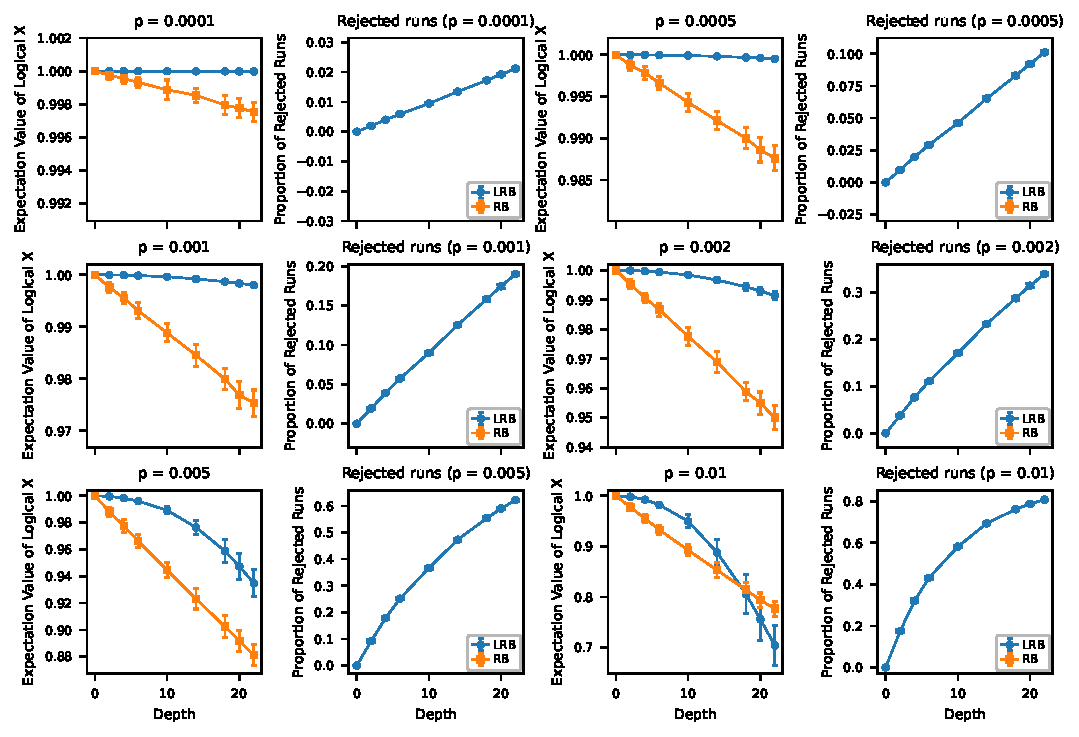
\includegraphics[width=0.95\textwidth]{figures/sdim140/si1000-1anc-const-0-nofit.pdf}
  \caption{Terminal postselection (const-0), one-ancilla layout, SI1000, at six values of $p$ from $10^{-4}$ to $10^{-2}$. In each pair of panels, the left panel shows the accepted $\langle \bar{X} \rangle$ of LRB-D (blue) and $\langle Z \rangle$ of physical RB under SI1000 at the same $p$ (orange) versus depth $m$, and the right panel shows the fraction of rejected LRB-D shots. The axis label ``Expectation Value of Logical X'' refers to LRB-D; for physical RB the plotted quantity is $\langle Z \rangle$. Error bars on $\langle \bar{X} \rangle$ and $\langle Z \rangle$ are standard deviations over the 30 sequences, and error bars on the rejected fraction are standard errors. The legend of each pair sits in its right panel and labels the curves of the left panel. Physical RB rejects no shots, so the right panel shows only LRB-D. No fits are drawn, since the LRB-D traces are not single exponentials.}
  \label{fig:const0_si1000_1anc}
\end{figure}

\begin{figure}[tb]
  \centering
  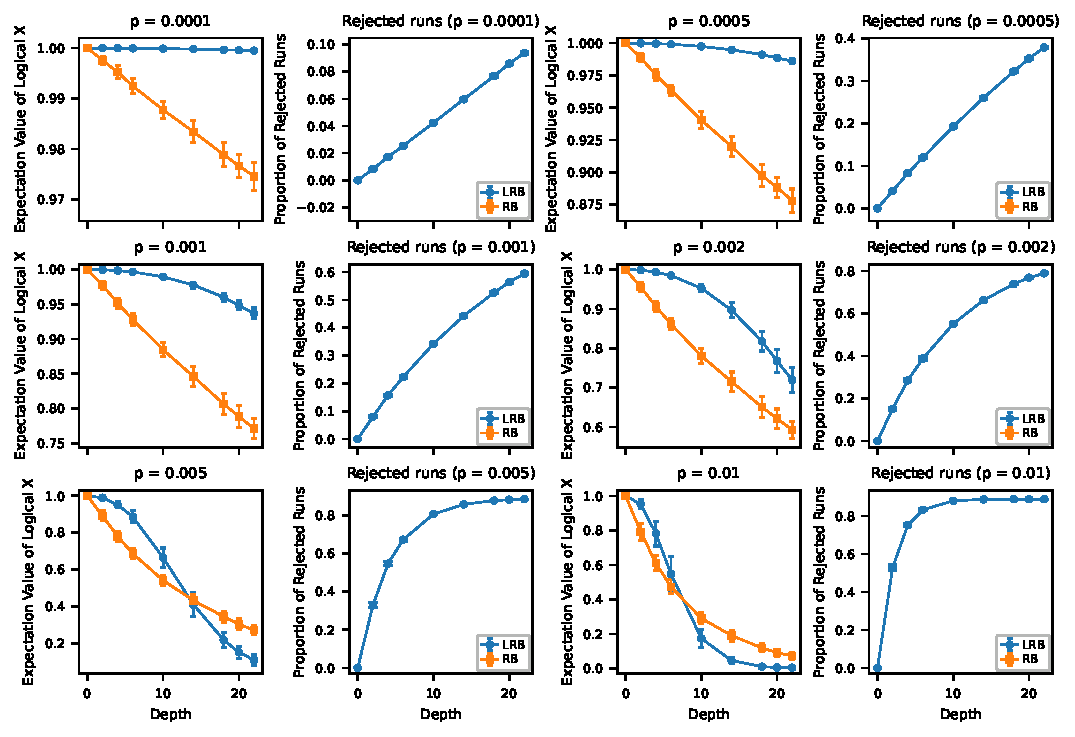
\includegraphics[width=0.95\textwidth]{figures/sdim140/sd6-1anc-const-0-nofit.pdf}
  \caption{Terminal postselection (const-0), one-ancilla layout, SD6, with panels as in \autoref{fig:const0_si1000_1anc}. The RB baseline runs under SD6 at the same $p$. At large $p m$ the rejected fraction approaches $8/9$, the value for uniformly random $X$-type syndromes, and the accepted $\langle \bar{X} \rangle$ approaches zero.}
  \label{fig:const0_sd6_1anc}
\end{figure}

The LRB-D traces stay flat at small depth and then bend down. At small $p$ the deficit $1 - \langle \bar{X} \rangle$ grows quadratically in both $m$ and $p$. Under SI1000 at $p = 10^{-3}$ it is $1.7\times10^{-5}$ at $m = 2$, $3.7\times10^{-4}$ at $m = 10$ and $2.0\times10^{-3}$ at $m = 22$. From $m = 2$ to $m = 10$ it grows by a factor of 22, while the RB deficit grows by a factor of 4.6, from $2.4\times10^{-3}$ to $1.1\times10^{-2}$. At $m = 10$, doubling $p$ from $5\times10^{-4}$ to $10^{-3}$ multiplies the LRB-D deficit by 4.0. SD6 behaves the same way. At $p = 10^{-3}$ the deficit grows by a factor of 28 from $m = 2$ to $m = 10$, from $3.8\times10^{-4}$ to $1.06\times10^{-2}$. Second-order growth in $p$ means that, to leading order, an accepted shot with a wrong readout carries two faults. This is what one expects if every single fault that changes the $X$-basis readout also leaves a nontrivial $X$-type syndrome, so that an accepted failure needs a second fault that restores trivial syndromes while leaving a logical error.

The shape of the traces also bears on the representation-theoretic picture of \autoref{sub:irreps}. Because $\langle \bar{X} \rangle = 1$ at $m = 0$, a single decay mode would give $1 - \langle \bar{X} \rangle \approx m(1-f)$ at small depth, which is linear in $m$. A quadratic onset requires several modes whose first-order contributions cancel. The encoded twirled channel has $m_{triv} + m_{pauli} = 2542$ relevant eigenvalues instead of two, and without intermediate checks one fault can carry the state into a syndrome sector from which a later fault returns it to trivial syndromes with a logical error. The data do not resolve individual modes. They show only that one mode does not describe terminal postselection, and we therefore extract no decay rate from it.

The rejected fraction grows with $m$ and $p$. Under SI1000 at $p = 5\times10^{-3}$ it is 9.2\% at $m = 2$, 37\% at $m = 10$ and 62\% at $m = 22$. Under SD6 it saturates near $8/9 \approx 0.889$, the value expected when the two $X$-type syndromes are uniformly distributed over their nine joint outcomes and only one outcome is accepted. At $p = 10^{-2}$ and $m = 22$ the rejected fraction is 0.8889, and the accepted shots retain almost no logical information, with $\langle \bar{X} \rangle = 0.0048$.

Because the LRB-D deficit grows faster than linearly in $m$ while the RB deficit grows linearly, the accepted $\langle \bar{X} \rangle$ falls below the RB $\langle Z \rangle$ at a depth that shrinks as $p$ grows. Under SI1000 the LRB-D value lies below RB at $m = 22$ for every $p \ge 10^{-2}$, but not at $7.5\times10^{-3}$, and at $m = 10$ for every $p \ge 2\times10^{-2}$, but not at $1.5\times10^{-2}$. Under SD6 it lies below RB at $m = 22$ for every $p \ge 5\times10^{-3}$, but not at $2\times10^{-3}$, and at $m = 10$ for every $p \ge 7.5\times10^{-3}$, but not at $5\times10^{-3}$.

Terminal postselection decays much faster under SD6 than under SI1000. At $p = 10^{-3}$ and $m = 22$ the LRB-D deficit is $6.3\times10^{-2}$ under SD6 and $2.0\times10^{-3}$ under SI1000, a factor of 32. The expected number of faults in a logical Clifford grows by a factor of five from SI1000 to SD6 ($5.7p$ to $29p$), and with second-order failures this alone predicts a factor of about 25. The RB baseline degrades as well, from a deficit of $0.025$ to $0.229$ at the same point.

\subsection{Uniform-Interval Postselection}
\label{sub:interval_results}

Under uniform-interval postselection with interval $k$, a shot is kept only if the check rounds after forward Cliffords $k, 2k, \dots$ and the final round all return trivial syndromes. The check round after every forward Clifford is present for every $k$, so all schedules share the same circuits and the same noise and differ only in the filter. For every $k$ the $m$ inverse Cliffords run without intermediate checks and are filtered only by the final round.

\paragraph{Interval $k = 1$.}
\autoref{fig:unif1_si1000_1anc} and \autoref{fig:unif1_sd6_1anc} show $k = 1$ in the one-ancilla layout. The accepted $\langle \bar{X} \rangle$ decays slowly. Under SI1000 the zero-offset fits follow the data closely, with $\chi^2 = 0.29$ and $0.43$ over nine depths at $p = 10^{-3}$ and $5\times10^{-3}$. Here $\chi^2$ is the weighted sum of squared residuals, with weights set by the variance over sequences rather than the variance of the mean, and it is not divided by the number of degrees of freedom. We use it only to compare schedules at the same $p$. Under SD6 the fits are worse at small $p$, with $\chi^2 = 6.6$ at $p = 10^{-3}$ and $15$ at $2\times10^{-3}$ over nine depths. The decay steepens with depth. At $p = 10^{-3}$, $\langle \bar{X} \rangle$ drops by $6.6\times10^{-5}$ per unit depth between $m = 0$ and $6$ and by $3.0\times10^{-4}$ per unit depth between $m = 18$ and $22$. This is consistent with the unfiltered inverse half, in which pairs of faults accumulate quadratically in $m$ as under terminal postselection, and with the five times larger fault budget of an SD6 logical Clifford. Frequent filtering thus removes most of the syndrome memory behind the multi-mode behavior of \autoref{sub:terminal_results}, but not all of it.

\begin{figure}[tb]
  \centering
  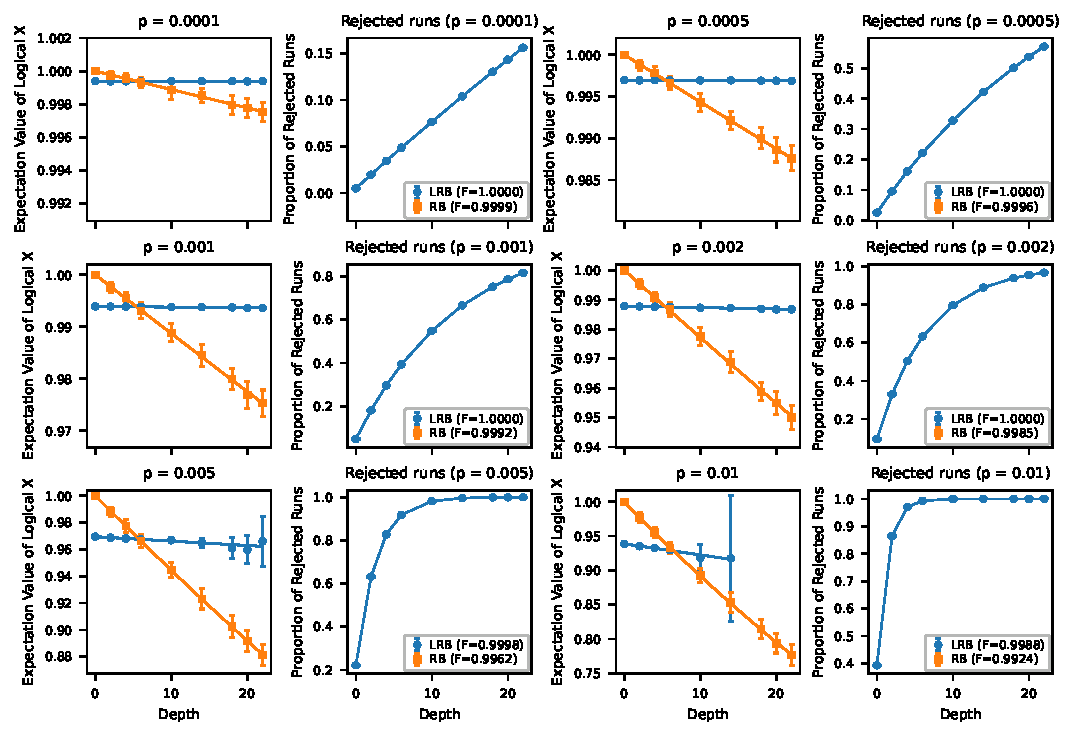
\includegraphics[width=0.95\textwidth]{figures/sdim140/si1000-1anc-unif-1-fit.pdf}
  \caption{Uniform-interval postselection with interval $k = 1$, one-ancilla layout, SI1000. Panels and error bars as in \autoref{fig:const0_si1000_1anc}. The lines are zero-offset fits $F(m) = A f^m$ to LRB-D (blue) and RB (orange), and the legends in the right panels give $\bar{F}$ per unit of depth. Missing LRB-D points at large $m$ and $p$ are depths at which some sequence keeps no shot.}
  \label{fig:unif1_si1000_1anc}
\end{figure}

\begin{figure}[tb]
  \centering
  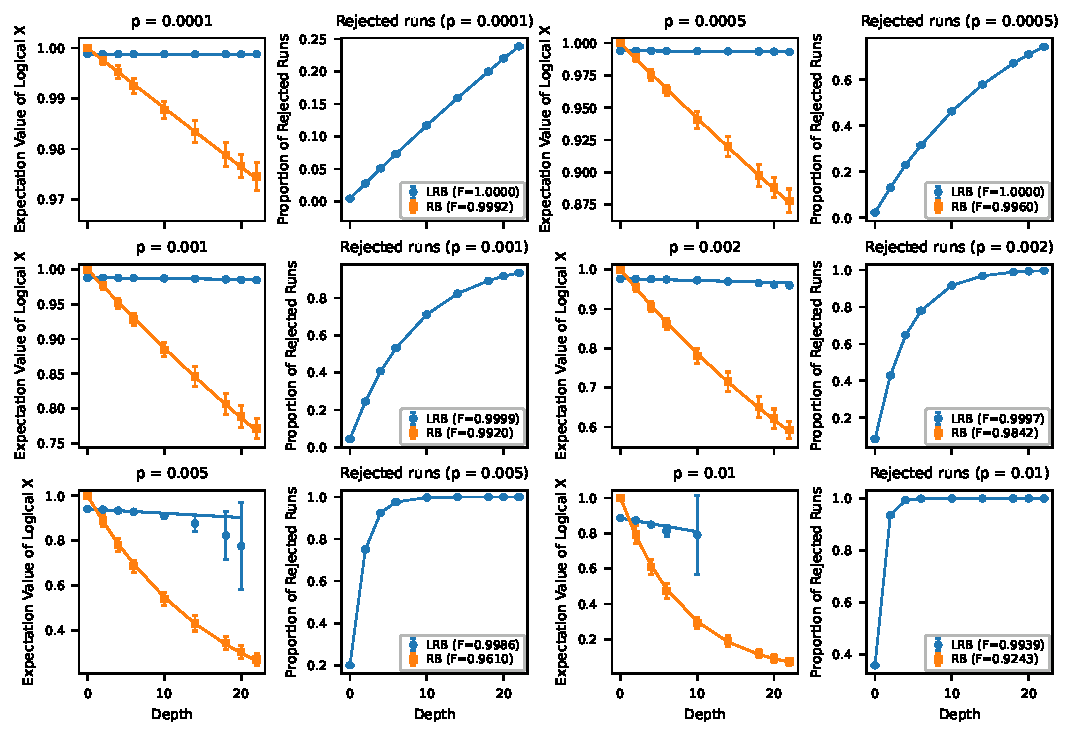
\includegraphics[width=0.95\textwidth]{figures/sdim140/sd6-1anc-unif-1-fit.pdf}
  \caption{Uniform-interval postselection with interval $k = 1$, one-ancilla layout, SD6, with panels, fits and legends as in \autoref{fig:unif1_si1000_1anc}. The RB baseline runs under SD6 at the same $p$, so its gates fail with probability $p$ and it decays ten times faster than under SI1000.}
  \label{fig:unif1_sd6_1anc}
\end{figure}

\autoref{tab:k1_error_rates} compares the fitted error rates with RB at four values of $p$. At $p = 5\times10^{-3}$ the average logical fidelity per unit depth is $\bar{F} = 0.99977$ against $0.9962$ for RB under SI1000, and $0.9986$ against $0.961$ under SD6. Between $p = 5\times10^{-4}$ and $2\times10^{-3}$ the LRB-D error grows as $p^{2.0}$ under SI1000 and $p^{1.9}$ under SD6, while the RB error grows as $p^{1.0}$ under both. Quadratic scaling is what one expects from a distance-2 code with postselection, since an accepted logical error needs two faults. The ratio $r_{\mathrm{RB}}/r_{\mathrm{LRB}}$ falls from 92 (SI1000) and 96 (SD6) at $p = 10^{-3}$ to 2.1 and 4.3 at $p = 2\times10^{-2}$. Under SD6 this is close to $1/p$. Under SI1000 the ratio falls faster, roughly as $p^{-1.3}$, because there the LRB-D error grows faster than $p^2$ above $p = 5\times10^{-3}$, as $p^{2.4}$ to $10^{-2}$ and $p^{2.6}$ from there to $2\times10^{-2}$.

\begin{table}[H]
  \centering
  \small
  \begin{tabular}{c|ccc|ccc}
    \hline
    & \multicolumn{3}{c|}{SI1000} & \multicolumn{3}{c}{SD6} \\
    $p$ & $r_{\mathrm{LRB}}$ & $r_{\mathrm{RB}}$ & depths & $r_{\mathrm{LRB}}$ & $r_{\mathrm{RB}}$ & depths \\
    \hline
    $10^{-3}$ & $(8.3 \pm 0.8)\times10^{-6}$ & $7.6\times10^{-4}$ & 9 & $(8.26 \pm 0.18)\times10^{-5}$ & $8.0\times10^{-3}$ & 9 \\
    $5\times10^{-3}$ & $(2.27 \pm 0.12)\times10^{-4}$ & $3.8\times10^{-3}$ & 9 & $(1.38 \pm 0.04)\times10^{-3}$ & $3.9\times10^{-2}$ & 8 \\
    $10^{-2}$ & $(1.16 \pm 0.04)\times10^{-3}$ & $7.6\times10^{-3}$ & 6 & $(6.05 \pm 0.20)\times10^{-3}$ & $7.6\times10^{-2}$ & 5 \\
    $2\times10^{-2}$ & $(7.15 \pm 0.24)\times10^{-3}$ & $1.5\times10^{-2}$ & 4 & $(3.29 \pm 0.21)\times10^{-2}$ & $1.4\times10^{-1}$ & 3 \\
    \hline
  \end{tabular}
  \caption{Fitted error rates per unit of depth for LRB-D with $k = 1$ in the one-ancilla layout ($r_{\mathrm{LRB}}$, with bootstrap standard deviation) and for physical RB under the same model at the same $p$ ($r_{\mathrm{RB}}$). The columns ``depths'' give the number of depths in the LRB-D fit. All values come from the production runs, and all RB fits use nine depths.}
  \label{tab:k1_error_rates}
\end{table}

The LRB-D traces start below one. At $m = 0$ the circuit consists of the ideal preparation, one noisy check round and the ideal readout. The accepted $\langle \bar{X} \rangle$ at $m = 0$ is $0.9939$, $0.9695$ and $0.9387$ at $p = 10^{-3}$, $5\times10^{-3}$ and $10^{-2}$ under SI1000, and $0.9881$, $0.9415$ and $0.8856$ under SD6. The deficit is first order in $p$, about $6p$ under SI1000 and $12p$ under SD6. It comes from faults on the data qutrits after their last two-qutrit gate of the round, including the idle noise during the final readout moment. A fault there that changes the logical readout leaves every syndrome of the round trivial, and no later round follows. Every depth ends with the same final round, so this loss enters as a common factor that the fitted amplitude absorbs ($A = 0.9695$ under SI1000 at $p = 5\times10^{-3}$), and to leading order it does not bias $f$. Because the RB trace starts at one, the raw curves cross at small depth, between $m = 4$ and $6$ under SI1000 at $p = 5\times10^{-3}$, although the LRB-D decay there is 17 times slower. We therefore compare decay rates rather than raw values.

The price of $k = 1$ is a fast-growing rejection. Under SI1000 at $p = 5\times10^{-3}$, 22\% of the shots are rejected at $m = 0$, 63\% at $m = 2$, 98.1\% at $m = 10$ and 99.98\% at $m = 22$, which leaves about 200 of $10^6$ shots per sequence. At $p = 10^{-3}$ the rejected fractions at the same depths are 4.9\%, 18\%, 55\% and 82\%. Under SD6 at $p = 5\times10^{-3}$ they are 20\% at $m = 0$, 75\% at $m = 2$ and 99.8\% at $m = 10$, and at $m = 22$ some sequence keeps no shot.

\paragraph{Intervals $k = 2$ to $4$ and beyond.}
\autoref{fig:unif2_si1000_1anc} to \autoref{fig:unif4_sd6_1anc} in \autoref{sec:additional-results} show $k = 2$, $3$ and $4$ in the one-ancilla layout. Fewer filters raise both the acceptance and the error per unit depth. Under SI1000 at $p = 5\times10^{-3}$, the rejected fraction at $m = 10$ falls from 98.1\% at $k = 1$ to 96.0\%, 94.6\% and 93.7\% at $k = 2$, $3$ and $4$, while the fitted LRB-D error rises from $2.3\times10^{-4}$ to $3.9\times10^{-4}$, $6.6\times10^{-4}$ and $9.3\times10^{-4}$. Under SD6 at the same $p$ the error rises from $1.4\times10^{-3}$ to $2.0\times10^{-3}$, $3.8\times10^{-3}$ and $5.3\times10^{-3}$.

Under SI1000 the fit quality changes in a step between $k = 2$ and $k = 3$. At $p = 5\times10^{-3}$, $\chi^2$ is $0.43$, $0.39$, $12.6$ and $9.1$ for $k = 1$ to $4$, all over nine depths. Under SD6, $\chi^2$ already exceeds 4 at $k = 1$ and grows more gradually with $k$, as $4.8$ (eight depths), $7.5$, $14.8$ and $24.8$ at the same $p$. The SI1000 step has a structural origin. For $k = 1$ and $2$ every depth of the production grid is a multiple of $k$, so the last forward Clifford is always followed by a filtered round. For $k \ge 3$ the number $m \bmod k$ of forward Cliffords after the last filtered intermediate round varies irregularly along the grid, as $0, 2, 1, 0, 1, 2, 0, 2, 1$ for $k = 3$, and the accepted $\langle \bar{X} \rangle$ develops small steps, so that a single exponential describes it only approximately. Under SD6 at $p = 10^{-3}$ and $k = 3$, for example, $\langle \bar{X} \rangle$ drops by $1.8\times10^{-4}$ from $m = 14$ to $18$, where this count falls from 2 to 0, and by $2.2\times10^{-3}$ from $m = 18$ to $20$, where it rises to 2. The second drop spans half the depth of the first and is twelve times larger, while the standard errors of these points are about $10^{-4}$. The extension runs also contain the odd depths $1$ and $3$, at which the $k = 2$ traces show the same steps, and their $k \ge 2$ fits therefore use only the even depths (\autoref{sub:pseudo_thresholds}).

Beyond $k = 4$, $\chi^2$ keeps growing. At $p = 5\times10^{-3}$ it reaches $116$ at $k = 10$ and $1213$ at $k = 22$ under SI1000, and $217$ and $3522$ under SD6, all over nine depths. Large intervals approach the case of a single filtered round at the end of the sequence, and the traces inherit the multi-mode behavior of terminal postselection. A fit to Eq.~\eqref{eq:fseq} then summarizes the trend but no longer estimates a logical error rate, so we restrict the quantitative analysis to $k \le 4$.

\paragraph{Fits at large $p$.}
In the production runs, the LRB-D fits rest on few depths from $p = 0.02$ on, because at larger depths some sequence keeps no shot. There the $k = 1$ fits use four depths at $p = 0.02$, three at $0.03$ and two at $0.04$ under SI1000, and three at $0.02$ and two at $0.03$ under SD6. The extension runs, at $p \ge 0.015$ under SI1000 and $p \ge 0.025$ under SD6, have more shots per depth but stop at $m = 6$, and their $k = 1$ fits use three to six depths under SI1000 and two to five under SD6. Unless $f$ reaches its bound of one, a two-point fit passes through both points exactly ($\chi^2 < 10^{-9}$). It says nothing about whether the decay is exponential, and its bootstrap interval reflects only the statistical errors of the two points. In addition, the per-sequence modulus $\lvert P_0 + \omega P_1 + \omega^2 P_2 \rvert$ is biased upward when only a few shots survive, since it is positive even for uniformly random outcomes. Under SD6 with $k = 4$ at $p = 0.02$, for example, the point at $m = 10$ rests on an average of 3.6 accepted shots per sequence and gives $\langle \bar{X} \rangle = 0.55$, above the value $0.39$ at $m = 2$. Error rates of the production runs at $p \ge 0.02$, and the SD6 pseudo-thresholds whose bracketing fits rest on few depths (\autoref{sub:pseudo_thresholds}), carry this systematic caveat in addition to their bootstrap errors.

\subsection{Pseudo-Thresholds}
\label{sub:pseudo_thresholds}

For each interval $k$ we define the pseudo-threshold $p^\star(k)$ as the value of $p$ at which the fitted LRB-D error rate equals the fitted error rate of physical RB under the same noise model. Below $p^\star(k)$ the postselected logical qutrit has the lower error per unit depth. In practice we locate $p^\star(k)$ as the onset of the regime in which the LRB-D error stays at or above the RB error, within a tolerance of $5\times10^{-4}$, at every larger $p$ on the grid, and we interpolate the difference linearly between the two bracketing grid points. The search skips the lowest grid points, where both error rates are below $2\times10^{-3}$. Before the search we cut the high-$p$ tail at the first point where the fitted LRB-D error drops below its running maximum by more than $0.01$ or 25\%, whichever is larger, since such drops come from fits starved of accepted shots. For both models the search runs on the merged grids of \autoref{sub:results_setup}, with the production fits at $p < p_{\mathrm{split}}$ and the extension fits from $p_{\mathrm{split}}$ to $0.05$ (SI1000, $p_{\mathrm{split}} = 0.015$) or $0.06$ (SD6, $p_{\mathrm{split}} = 0.025$). For $k \ge 2$ the extension fits use only the even depths $m = 0$, $2$, $4$ and $6$, for the reason given below. The uncertainty of $p^\star(k)$ is one standard error from the bootstrap over the random Clifford sequences of \autoref{sub:fit_model}, with 1000 replicates. Each replicate resamples the sequences of the production and extension runs, LRB-D and RB alike, refits every curve, and repeats the search described here, tail cut included.

% Bracketing fits, depth counts and accepted shots: paper-rework/scratch/writer-evendepth/analysis.py (sections A, A2); lib.py there applies the even-depth rule and reproduces all 16 canonical values of LRB-experiment-data-slurm/comparisons/pseudo-thresholds-current.csv (verify.out)
\autoref{tab:pseudo_thresholds} lists $p^\star(k)$ for the four configurations. All sixteen entries are genuine crossings, bracketed by grid points at which the LRB-D error is below and above the RB error, and we quote them with one standard error from the sequence bootstrap. Every LRB-D fit that brackets an SI1000 crossing uses four to eight depths, and under SD6 those that bracket $p^\star(1)$ and $p^\star(2)$ use three to five. Near $p^\star(1)$ and $p^\star(2)$ both bracketing fits come from the extension and cover only $m \le 6$. The largest depths of some bracketing fits keep few accepted shots (\autoref{sub:postselection_cost}). Under SD6, where these fits rest on as few as three depths, the systematic caveats of \autoref{sub:interval_results} therefore apply. Under SI1000 the few-shot points carry almost no weight in the fit.

Under SI1000 the crossings at $k = 1$, $2$ and $3$ lie between extension points, at $0.0275$ and $0.03$ for $k = 1$, $0.0225$ and $0.025$ for $k = 2$, and $0.015$ and $0.0175$ for $k = 3$. The one-ancilla crossing at $k = 4$ lies between the production point $0.0125$ and the extension point $0.015$, and the two-ancilla crossing at $k = 4$ between the production points $0.01$ and $0.0125$. Under SD6 both values of $p^\star(1)$ lie between the extension points $0.035$ and $0.04$, and both values of $p^\star(2)$ between the extension points $0.025$ and $0.03$. The SD6 values at $k = 3$ and $4$ lie between production grid points, and the extension only confirms that the LRB-D error stays above RB beyond them. Two of the crossings sit on grid points. In the two-ancilla SI1000 configuration with $k = 3$, the two error rates agree within the tolerance at the extension grid point $0.015$ ($0.0113$ against $0.0116$), and the sign change of their difference lies at $0.0152$ by linear interpolation. In the two-ancilla SD6 configuration with $k = 4$, they agree at the production grid point $0.0125$ ($0.0908$ against $0.0910$), and the sign change lies at $0.01251$.

\begin{table}[htb]
  \centering
  \begin{tabular}{c|cc|cc}
    \hline
    & \multicolumn{2}{c|}{one-ancilla layout} & \multicolumn{2}{c}{two-ancilla layout} \\
    $k$ & SI1000 & SD6 & SI1000 & SD6 \\
    \hline
    1 & $0.0292 \pm 0.0006$ & $0.0399 \pm 0.0015$ & $0.0288 \pm 0.0006$ & $0.0360 \pm 0.0013$ \\
    2 & $0.0239 \pm 0.0005$ & $0.0269 \pm 0.0007$ & $0.0228 \pm 0.0005$ & $0.0251 \pm 0.0015$ \\
    3 & $0.0166 \pm 0.0004$ & $0.0181 \pm 0.0006$ & $0.0150 \pm 0.0003$ & $0.0145 \pm 0.0004$ \\
    4 & $0.0132 \pm 0.0002$ & $0.0155 \pm 0.0004$ & $0.0119 \pm 0.0003$ & $0.0125 \pm 0.0003$ \\
    \hline
  \end{tabular}
  \caption{Pseudo-thresholds $p^\star(k)$ against physical RB under the same noise model at the same $p$. Uncertainties are one standard error (68\% confidence), from a bootstrap over the random Clifford sequences (\autoref{sub:fit_model}). All entries are genuine crossings. All entries use the production fits at $p < p_{\mathrm{split}}$ and the high-$p$ extension (depths $0, 1, 2, 3, 4, 6$; $2\times10^7$ shots per sequence and depth; 30 new sequences) at $p \ge p_{\mathrm{split}}$, with $p_{\mathrm{split}} = 0.015$ under SI1000 and $0.025$ under SD6. For $k \ge 2$ the extension fits use only the even depths $0, 2, 4, 6$, as in the production grid, which removes the odd depths at which the $k = 2$ traces show steps. Where production and extension overlap, their fitted RB errors differ by 1 to 4\% under SI1000 and by 4 to 8.5\% under SD6 (\autoref{sub:results_setup}). The two-ancilla entries at $k = 3$ (SI1000) and $k = 4$ (SD6) sit on grid points within the tolerance of the search.}
  \label{tab:pseudo_thresholds}
\end{table}

% Even-depth rule: applied by scripts/merge_highp_threshold_extension.py (class EvenDepthsForSparseChecks)
The extension fits for $k \ge 2$ use only even depths because of the steps described in \autoref{sub:interval_results}. At a depth that is not a multiple of $k$, the last $m \bmod k$ forward Cliffords run without a filtered round before the final round (one Clifford at the odd depths for $k = 2$), so the accepted $\langle \bar{X} \rangle$ at such depths lies on a different curve. For $k = 2$ these are the odd depths $1$ and $3$ of the extension grid. All production depths are even, so the rule gives both data sets the same depth structure. For $k = 3$ and $4$ the even depths still include depths that are not multiples of $k$, $m = 2$ and $4$ for $k = 3$ and $m = 2$ and $6$ for $k = 4$, as the production grid does.

% Fit quality near the SI1000 crossings: lrb_chi2 / (lrb_n_points - 2) of the merged tables, LRB-experiment-data-slurm/comparisons/sdim140-si1000-highp-merged/{one,two}-ancilla-si1000/unif_lrb_vs_rb_table_merged.csv, p = 0.015 to 0.035
Near the SI1000 crossings the single-exponential fits still describe the accepted decays well at $k = 1$ and $2$. Between $p = 0.015$ and $0.035$ their $\chi^2$ per degree of freedom, defined as in \autoref{sub:interval_results}, is $0.1$ to $0.9$ in both layouts. At $k = 3$ and $4$ it is $1$ to $8$, because of the steps at depths that are not multiples of $k$.

\autoref{fig:threshold_grid_si1000_1anc} and \autoref{fig:threshold_grid_sd6_1anc} show the construction for the one-ancilla layout, and \autoref{fig:pstar_vs_k} collects $p^\star(k)$ for all four configurations. The corresponding two-ancilla figures are \autoref{fig:threshold_grid_si1000_2anc} and \autoref{fig:threshold_grid_sd6_2anc}.

\begin{figure}[htb]
  \centering
  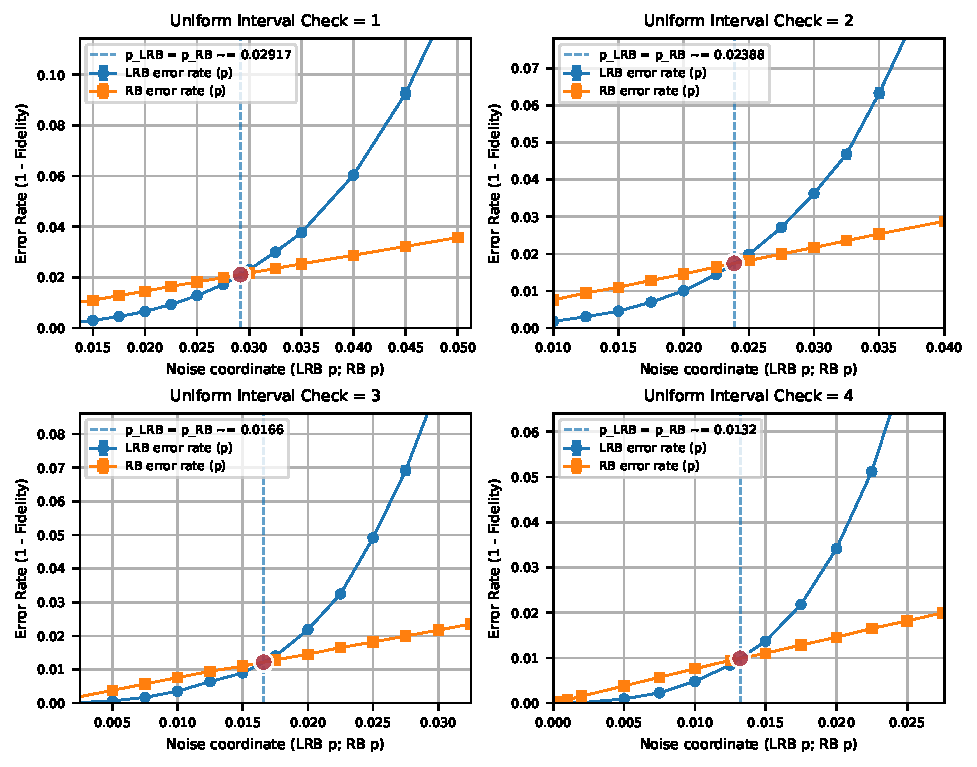
\includegraphics[width=0.75\textwidth]{figures/sdim140/si1000-1anc-threshold-grid.pdf}
  \caption{Pseudo-threshold construction, one-ancilla layout, SI1000. Fitted error rate per unit of depth of LRB-D (blue) and of physical RB under SI1000 at the same $p$ (orange) versus $p$, for $k = 1$, $2$, $3$ and $4$, with 68\% bootstrap intervals. Points at $p < 0.015$ come from the production run, and points at $p \ge 0.015$ from the high-$p$ extension. There the $k = 1$ fits use those of the depths $0, 1, 2, 3, 4$ and $6$ at which every sequence keeps at least one shot, four to six depths, and the $k \ge 2$ fits use the even depths $0, 2, 4$ and $6$, three or four depths (\autoref{sub:results_setup}). The $k = 1$ panel shows only extension points. The vertical line and the marker give $p^\star(k) = 0.0292$, $0.0239$, $0.0166$ and $0.0132$, all genuine crossings. The RB error rises about linearly in $p$, and the LRB-D error rises faster and crosses it. The $k = 1$, $2$ and $3$ crossings lie between extension points, and the $k = 4$ crossing lies between the production point $0.0125$ and the extension point $0.015$. The fits that bracket $p^\star(1)$ use six depths, and those that bracket $p^\star(2)$ and $p^\star(3)$ use four. For $k = 4$ the production fit at $p = 0.0125$ uses seven depths and the extension fit at $0.015$ uses four.}
  \label{fig:threshold_grid_si1000_1anc}
\end{figure}

\begin{figure}[htb]
  \centering
  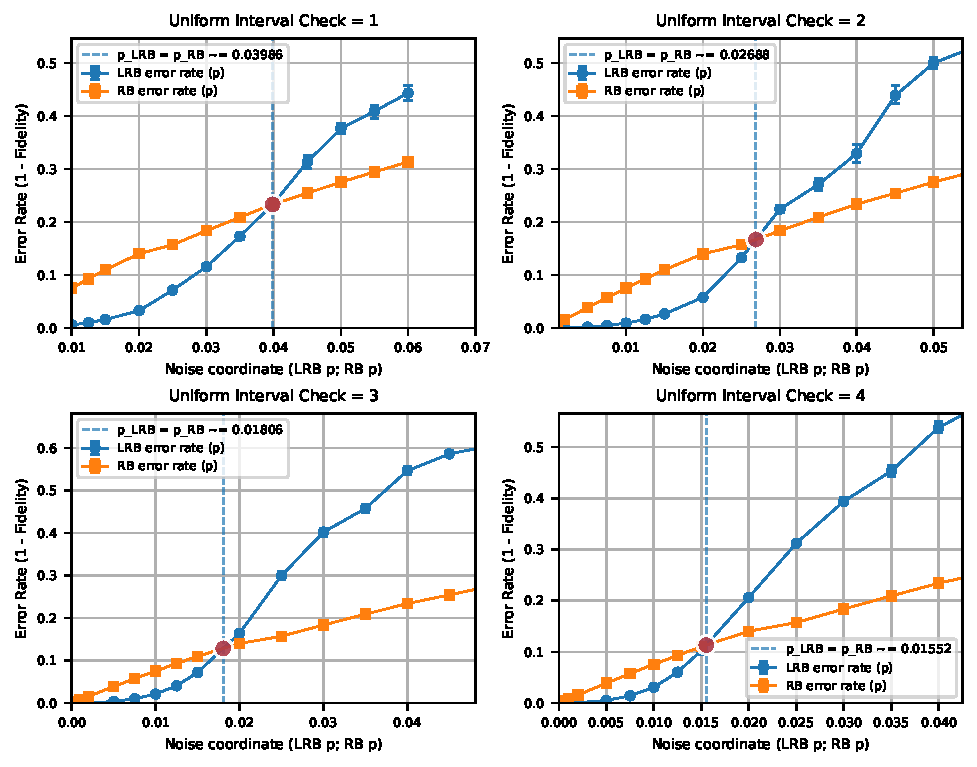
\includegraphics[width=0.75\textwidth]{figures/sdim140/sd6-1anc-threshold-grid.pdf}
  \caption{Pseudo-threshold construction, one-ancilla layout, SD6, with curves as in \autoref{fig:threshold_grid_si1000_1anc} and RB under SD6. Points at $p < 0.025$ come from the production run, and points at $p \ge 0.025$ from the high-$p$ extension. There the $k = 1$ fits use those extension depths at which every sequence keeps at least one shot, three to five depths with $m \le 4$, and the $k \ge 2$ fits use three or four of the even depths $0, 2, 4$ and $6$ (\autoref{sub:results_setup}). The markers are genuine crossings at $p^\star(k) = 0.0399$, $0.0269$, $0.0181$ and $0.0155$. The $k = 1$ and $2$ crossings lie between extension points, and the $k = 3$ and $4$ crossings between production points.}
  \label{fig:threshold_grid_sd6_1anc}
\end{figure}

\begin{figure}[htb]
  \centering
  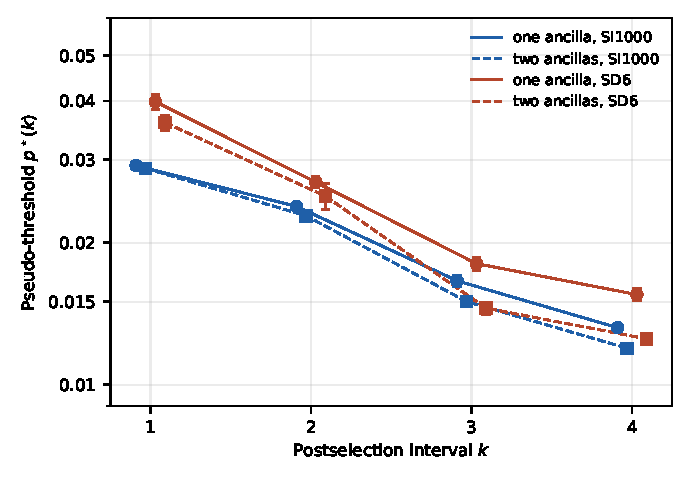
\includegraphics[width=0.65\textwidth]{figures/sdim140/pstar-vs-k-four-configs.pdf}
  \caption{Pseudo-threshold $p^\star(k)$ versus postselection interval $k$ for the one-ancilla (circles, solid lines) and two-ancilla (squares, dashed lines) layouts under SI1000 (blue) and SD6 (red). All markers are genuine crossings. Error bars are one standard error (68\% confidence) from the bootstrap over the random Clifford sequences (\autoref{sub:fit_model}); bars that are not visible are smaller than the markers. The two-ancilla markers at $k = 3$ (SI1000) and $k = 4$ (SD6) sit on grid points within the tolerance of the search. All values use the production fits at $p < p_{\mathrm{split}}$ and the high-$p$ extension at $p \ge p_{\mathrm{split}}$, with $p_{\mathrm{split}} = 0.015$ under SI1000 and $0.025$ under SD6, and for $k \ge 2$ only the even extension depths (\autoref{sub:results_setup}). Markers are offset horizontally for legibility.}
  \label{fig:pstar_vs_k}
\end{figure}

% Factors from LRB-experiment-data-slurm/comparisons/pseudo-thresholds-current.csv; paired adjacent-interval gaps: LRB-experiment-data-slurm/comparisons/sequence-bootstrap/interval_gap_significance.csv, checked from the replicate files by paper-rework/scratch/writer-seq-se/paired.py (paired.out); SD6-versus-SI1000 gaps with standard errors in quadrature: paper-rework/scratch/lead/se_comparisons.py (se_comparisons.out), checked by paper-rework/scratch/writer-seq-se/check.py (check.out)
In every configuration $p^\star(k)$ falls with $k$. The decrease of $p^\star$ with the check interval is significant at 6 standard errors or more for every adjacent pair of intervals, with the bootstrap replicates paired over the shared sequences, whose common fluctuations largely cancel in the differences. The smallest steps, from $k = 3$ to $4$ under SD6, amount to 6.1 standard errors with one ancilla and 6.3 with two, and the ordering $p^\star(1) > p^\star(2) > p^\star(3) > p^\star(4)$ holds in all 1000 replicates of every configuration. In the one-ancilla layout it drops by a factor of 2.2 from $k = 1$ to $4$ under SI1000 ($0.0292$ to $0.0132$) and by a factor of 2.6 under SD6 ($0.0399$ to $0.0155$).
The circuits are identical for all $k$, so the drop reflects only which shots are kept. A fault that a skipped round would have flagged survives until the next filtered round. If a second fault arrives in between and the two combine into an error with trivial syndromes, for example a logical operator, no later round can detect it. Fewer filters therefore keep more shots that carry logical errors. The fitted LRB-D error at fixed $p$ grows with $k$ (\autoref{sub:interval_results}), while RB does not depend on $k$, and the crossing moves to smaller $p$.
In the one-ancilla layout the factors from $k = 1$ to $2$, $2$ to $3$ and $3$ to $4$ are 1.22, 1.44 and 1.26 under SI1000 and 1.48, 1.49 and 1.16 under SD6.

In the one-ancilla layout, the SD6 pseudo-thresholds lie above the SI1000 values at every $k$. They are $0.0399$ against $0.0292$ at $k = 1$, $0.0269$ against $0.0239$ at $k = 2$, $0.0181$ against $0.0166$ at $k = 3$ and $0.0155$ against $0.0132$ at $k = 4$, higher by $36.7 \pm 5.7\%$, $12.6 \pm 3.7\%$, $8.8 \pm 4.5\%$ and $17.6 \pm 3.8\%$, or 6.5, 3.4, 1.9 and 4.6 combined standard errors (the two standard errors added in quadrature). The ordering is therefore resolved at $k = 1$, $2$ and $4$, and at $k = 3$ only at the level of two standard errors. In the two-ancilla layout the SD6 value is higher by $25.1 \pm 5.3\%$ at $k = 1$. At $k = 2$, $3$ and $4$ the SD6 values differ from the SI1000 values by $+10.1 \pm 7.2\%$, $-3.1 \pm 3.5\%$ and $+4.7 \pm 3.3\%$, within 1.4 standard errors, and there we do not resolve a difference between the models. This does not mean that the encoded circuits fare better under SD6. At $p = 10^{-2}$ and $k = 1$ the fitted LRB-D error is 5.2 times larger under SD6 than under SI1000 ($6.1\times10^{-3}$ against $1.2\times10^{-3}$). The RB baseline is 10 times worse ($7.6\times10^{-2}$ against $7.6\times10^{-3}$), because its one-qutrit gates fail with probability $p$ instead of $p/10$. A pseudo-threshold thus compares the code with a baseline whose quality depends on the noise model. SI1000 pairs the code with a physical qutrit whose gates are ten times cleaner than the two-qutrit gates that set $p$, and it is the more demanding comparison.

\subsection{One- and Two-Ancilla Layouts}
\label{sub:layout_comparison}

The two-ancilla layout measures the boundary stabilizers $G_1$ and $G_4$ through a relay ancilla (\autoref{sub:ancilla_layouts}). Per check round this raises the number of two-qutrit gates from 12 to 16, the number of ancilla resets and readouts from 4 to 6, and the number of moments from 9 to 11. Both relay readouts must also return 0. The expected number of faults per round rises from $68p$ to $91p$ under SI1000 and from $73p$ to $111p$ under SD6. The composition of the increase differs between the models. Under SI1000, $14p$ of the extra $23p$ are ancilla reset and readout flips, which shift recorded syndromes. Under SD6, $26p$ of the extra $38p$ come from 26 additional idle locations, which fail with probability $p$. Under SI1000 the same locations sit in gate moments and fail with probability $p/10$, so they add only $2.6p$.

The relay raises the rejection under both models. With one check round at $m = 0$ and $p = 5\times10^{-3}$, the rejected fraction grows from 22\% to 29\% under SI1000 and from 20\% to 29\% under SD6. Its effect on the error per unit depth differs. \autoref{fig:four_configs} compares the four configurations for $k = 1$. Under SI1000 the two layouts are nearly indistinguishable. At $p = 5\times10^{-3}$ the fitted LRB-D error is $2.5\times10^{-4}$ with two ancillas and $2.3\times10^{-4}$ with one, and at $p = 10^{-2}$ both are $1.16\times10^{-3}$. Under SD6 the relay costs more. At $p = 5\times10^{-3}$ the error rises from $1.38\times10^{-3}$ to $1.71\times10^{-3}$, and at $p = 10^{-2}$ from $6.1\times10^{-3}$ to $8.6\times10^{-3}$.

\begin{figure}[htb]
  \centering
  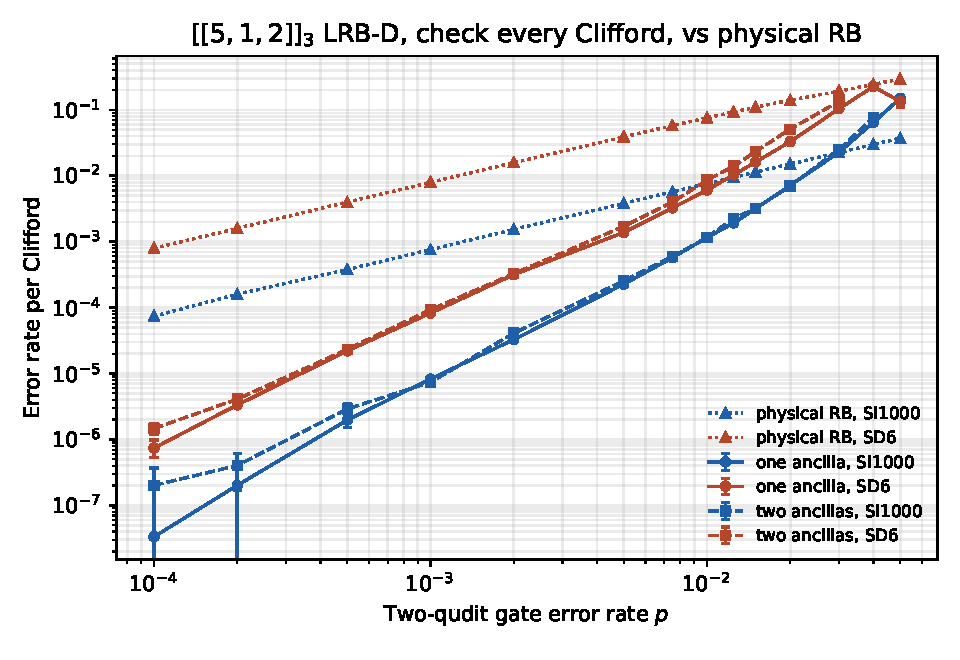
\includegraphics[width=0.7\textwidth]{figures/sdim140/four-configs-unif-1-lrb-vs-rb.pdf}
  \caption{Fitted error rate per unit of depth for LRB-D with $k = 1$ (a filtered check round after every forward Clifford) versus $p$, for the one-ancilla (solid) and two-ancilla (dashed) layouts under SI1000 (blue) and SD6 (red), together with physical RB under SI1000 and SD6 (dotted, triangles). The axis label ``per Clifford'' refers to one unit of depth, a forward logical Clifford with its mirror inverse. Likewise, ``check every Clifford'' in the title means a filtered check round after every forward Clifford, and the mirror inverse runs without checks. The RB curves come from the one-ancilla runs. The two-ancilla runs draw their own RB sequences, whose errors differ from these by a few percent (\autoref{sub:results_setup}). Error bars are 68\% bootstrap intervals. At small $p$ the LRB-D errors scale as $p^2$ and the RB errors as $p$. At $p = 10^{-4}$ the one-ancilla SI1000 value, $3\times10^{-8}$, sits at the resolution of the fit. From $p = 0.03$ on, the LRB-D fits rest on two or three depths. The downturn of the one-ancilla SD6 curve at $p = 0.05$ comes from such a fit, the two-ancilla SI1000 fit at $p = 0.05$ returns zero error and is not drawn, and the two-ancilla SD6 configuration has no fit above $p = 0.03$. All curves are fits to the production runs. The pseudo-thresholds of both models replace the production points at $p \ge 0.015$ (SI1000) and $p \ge 0.025$ (SD6) by fits to the high-$p$ extension, which for $k = 1$ use every extension depth that keeps shots (\autoref{fig:threshold_grid_si1000_1anc}, \autoref{fig:threshold_grid_sd6_1anc}, \autoref{fig:threshold_grid_si1000_2anc}, \autoref{fig:threshold_grid_sd6_2anc}). Under SI1000 they place the $k = 1$ crossings at $0.0292$ and $0.0288$, close to $p = 0.03$, where the production curves drawn here meet the RB curve. Under SD6 they place them at $0.0399$ and $0.0360$, where the production fits drawn here lie below RB or are missing.}
  \label{fig:four_configs}
\end{figure}

\autoref{tab:pseudo_thresholds} compares the pseudo-thresholds of the two layouts. Each layout is compared with the RB baseline of its own run, and these baselines differ by a few percent (\autoref{sub:results_setup}). The standard errors of $p^\star$ include the spread from the choice of the LRB-D and RB sequences, since the bootstrap resamples both, and the standard error of a gap combines those of the two runs in quadrature (\autoref{sub:fit_model}).
% Layout gaps against each run's own RB, with standard errors added in quadrature (independent runs): paper-rework/scratch/lead/se_comparisons.py (se_comparisons.out), from LRB-experiment-data-slurm/comparisons/pseudo-thresholds-current.csv; checked by paper-rework/scratch/writer-seq-se/check.py (check.out)
Under SI1000 the two-ancilla values lie below the one-ancilla values by $9.7 \pm 3.1\%$ at $k = 3$ and $9.6 \pm 2.4\%$ at $k = 4$, or 3.1 and 4.0 standard errors. At $k = 1$ and $2$ the gaps are $1.4 \pm 2.9\%$ and $4.5 \pm 2.9\%$, or 0.5 and 1.5 standard errors, so there we do not resolve a difference between the layouts.
Under SD6 the two-ancilla layout loses $19.6 \pm 3.4\%$ at $k = 3$ and $19.5 \pm 3.0\%$ at $k = 4$, with $0.0145$ against $0.0181$ and $0.0125$ against $0.0155$, or 5.7 and 6.6 standard errors. At $k = 1$ and $2$ it loses $9.7 \pm 4.7\%$ and $6.6 \pm 6.3\%$, with $0.0360$ against $0.0399$ and $0.0251$ against $0.0269$, or 2.1 and 1.1 standard errors. The SD6 gap at $k = 1$ is thus marginal, and at $k = 2$ we do not resolve a difference.
At $k = 3$ and $4$ the relay therefore costs about 10\% of $p^\star$ under SI1000 and about 20\% under SD6. The gaps of the two models differ by $9.9 \pm 4.7\%$ at $k = 3$ and $9.9 \pm 3.8\%$ at $k = 4$, or 2.1 and 2.6 standard errors. This ordering agrees with the noise budget of the relay: under SI1000 most of its added noise only triggers rejections, whereas under SD6 its idle locations add depolarizing noise at the full rate $p$. At $k = 1$ and $2$ the gaps of the two models differ by 1.5 and 0.3 standard errors and are not resolved. In both models the relay costs acceptance.

\subsection{Cost of Postselection and Conditional Interpretation}
\label{sub:postselection_cost}

Postselection is what allows us to benchmark the $[[5,1,2]]_3$ code without a decoder. The code detects every single-qutrit error but cannot correct them (\autoref{sub:lrb_d}), and discarding flagged shots avoids committing to a correction rule. The interval $k$ also provides a control that moves the LRB-D traces toward the multi-mode behavior of terminal postselection, as discussed in \autoref{sub:irreps}. Under SI1000 the decay is close to a single exponential at $k \le 2$ and approximately so at $k = 3$ and $4$ (\autoref{sub:interval_results}). Under SD6 it already steepens with depth at $k = 1$ (\autoref{sub:interval_results}).

The drawback is the sampling cost. In the one-ancilla SI1000 configuration with $k = 1$ at $p = 5\times10^{-3}$, about 200 of $10^6$ shots per sequence survive to $m = 22$ (\autoref{sub:interval_results}). Near the pseudo-threshold the cost is higher. In the production run at $p = 3\times10^{-2}$, 77\% of the shots are rejected at $m = 0$ and 99.74\% at $m = 2$, an average of 28 of $10^6$ shots per sequence survives to $m = 4$, and from $m = 6$ on some sequence keeps no shot. The pseudo-thresholds at $k = 1$ and $2$ therefore rest on the extension runs, which sample $2\times10^7$ shots per sequence and depth up to $m = 6$ (\autoref{sub:results_setup}).
% Depth counts and accepted shots of the bracketing fits: paper-rework/scratch/writer-evendepth/analysis.py (section A); spread over sequences of the one-ancilla k = 1 data at p = 0.03: paper-rework/scratch/writer-evendepth/extras.py (m = 0 diagnostics) and paper-rework/scratch/s2-physics-reviewer/c_misc.py (standard errors over the 30 sequences)
Under SI1000 the two fits that bracket $p^\star(1) = 0.0292$, at $p = 0.0275$ and $0.03$, use all six extension depths, but at $m = 6$ an average of only 23 and 6.7 shots per sequence survive. The two that bracket $p^\star(2) = 0.0239$, at $p = 0.0225$ and $0.025$, use the four even depths, and about 2300 and 890 shots per sequence survive to $m = 6$. With two ancillas the $k = 1$ fits at $p = 0.0275$ and $0.03$ use five depths, up to $m = 4$, where 80 and 26 shots per sequence survive, and the $k = 2$ fits at $p = 0.0225$ and $0.025$ use the four even depths, with about 300 and 95 shots per sequence at $m = 6$. These numbers measure the sampling cost. The few-shot points carry almost no weight in the fit, which weights each depth by the inverse variance over sequences: at $m = 6$ and $p = 0.03$ the one-ancilla $k = 1$ data scatter over sequences with a standard deviation of $0.23$, against $0.005$ to $0.03$ at $m = 1$ to $4$.
Under SD6 the fits that bracket $p^\star(1)$ come from the extension, at $p = 0.035$ and $0.04$, and rest on five and four of its depths with one ancilla and on three each with two ancillas. Their largest depths also keep few shots. With one ancilla at $p = 0.035$, the point at $m = 4$ rests on an average of 3.8 of $2\times10^7$ shots per sequence and gives $\langle \bar{X} \rangle = 0.68$, above $0.21$ at $m = 3$, which is the upward bias described in \autoref{sub:interval_results}. Larger $k$ lowers the cost. Under SI1000 at $p = 5\times10^{-3}$, $k = 4$ rejects 50\% of the shots at $m = 2$ and 94\% at $m = 10$, against 63\% and 98\% for $k = 1$, at the price of a larger error per unit depth and a lower pseudo-threshold.

LRB-D also reports a conditional quantity. The fitted error per unit depth describes the logical errors that pass every filtered round, that is, how well the logical state is preserved along the accepted trajectories. It is not the unconditional reliability of a computation of depth $m$, which succeeds only with the acceptance probability. It also leaves out the fixed loss at $m = 0$, which the fitted amplitude absorbs. This loss is about $6p$ (SI1000) or $12p$ (SD6) in the one-ancilla layout and about $6.5p$ or $15p$ in the two-ancilla layout. A comparison of an encoded qutrit with a physical one should therefore quote the error per unit depth together with the acceptance it requires.


\subsection{IQM QPU}


\appendix

% Additional figures for the circuit-level SI1000 and SD6 results.
% Numbers trace to paper-rework/facts/*.csv and the run folders listed in facts/runs.csv.

\section{Additional Results}
\label{sec:additional-results}

This appendix collects the figures that support \autoref{sec:results} but are not shown there. \autoref{fig:unif2_si1000_1anc} to \autoref{fig:unif4_sd6_1anc} show uniform-interval postselection with $k = 2$, $3$ and $4$ in the one-ancilla layout, discussed in \autoref{sub:interval_results}. \autoref{fig:const0_si1000_2anc} to \autoref{fig:unif1_sd6_2anc} show terminal postselection and uniform-interval postselection with $k = 1$ for the two-ancilla layout, and \autoref{fig:threshold_grid_si1000_2anc} and \autoref{fig:threshold_grid_sd6_2anc} show its pseudo-threshold construction, all discussed in \autoref{sub:layout_comparison}. In the depth-decay figures, \autoref{fig:unif2_si1000_1anc} to \autoref{fig:unif1_sd6_2anc}, the panels follow \autoref{fig:const0_si1000_1anc} and \autoref{fig:unif1_si1000_1anc}. Each pair of panels belongs to one of $p = 10^{-4}$, $5\times10^{-4}$, $10^{-3}$, $2\times10^{-3}$, $5\times10^{-3}$ and $10^{-2}$. The left panel shows the accepted $\langle \bar{X} \rangle$ of LRB-D (blue) and $\langle Z \rangle$ of physical RB under the same noise model at the same $p$ (orange) versus depth $m$, and the right panel shows the rejected fraction. The legend of each pair sits in its right panel and labels the curves of the left panel. Where fits are drawn, they are $F(m) = A f^m$, and the legends give $\bar{F}$ per unit of depth. The two threshold-grid figures follow \autoref{fig:threshold_grid_si1000_1anc} and \autoref{fig:threshold_grid_sd6_1anc}. All $\chi^2$ values quoted below are defined as in \autoref{sub:interval_results}.

\subsection{One-Ancilla Layout, Intervals \texorpdfstring{$k = 2$}{k = 2} to \texorpdfstring{$4$}{4}}

\begin{figure}[H]
  \centering
  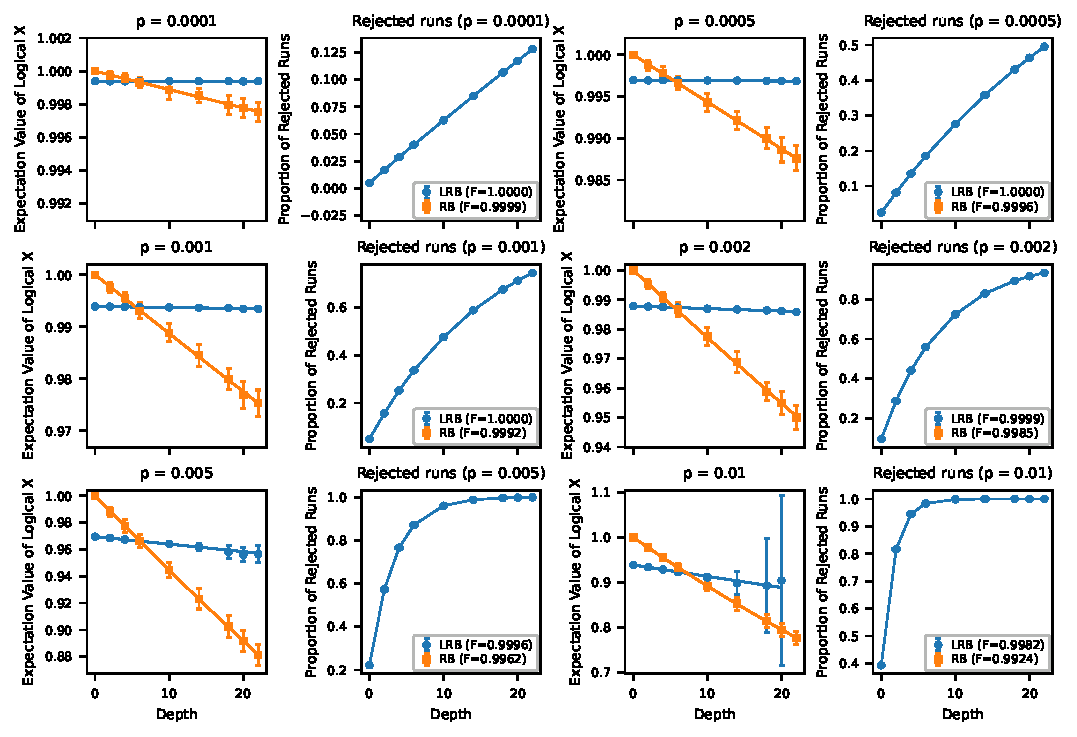
\includegraphics[width=0.78\textwidth]{figures/sdim140/si1000-1anc-unif-2-fit.pdf}
  \caption{Uniform-interval postselection with $k = 2$, one-ancilla layout, SI1000. Every depth on the grid is a multiple of 2, and the zero-offset fits stay close to the data ($\chi^2 = 0.39$ over nine depths at $p = 5\times10^{-3}$). At $p = 5\times10^{-3}$ the fitted error per unit depth is $3.9\times10^{-4}$, against $2.3\times10^{-4}$ for $k = 1$.}
  \label{fig:unif2_si1000_1anc}
\end{figure}

\begin{figure}[H]
  \centering
  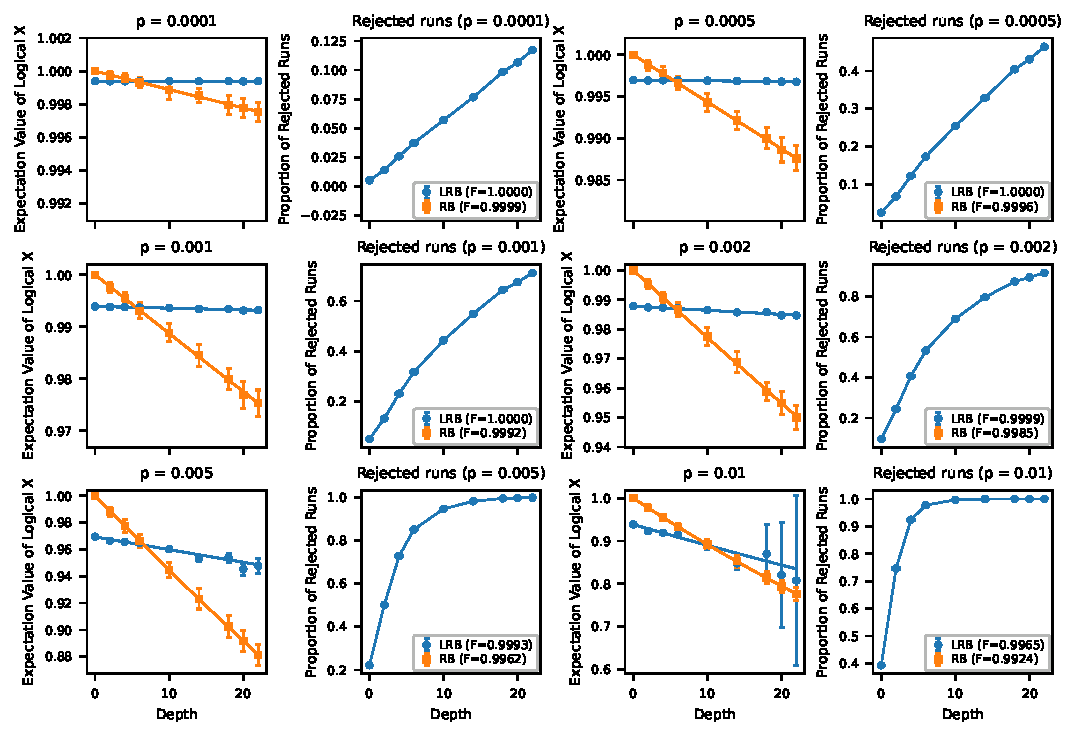
\includegraphics[width=0.78\textwidth]{figures/sdim140/si1000-1anc-unif-3-fit.pdf}
  \caption{Uniform-interval postselection with $k = 3$, one-ancilla layout, SI1000. The rejected fraction at fixed depth $m \ge 2$ is lower than for $k \le 2$, and the traces develop steps at depths that are not multiples of 3 ($\chi^2 = 12.6$ over nine depths at $p = 5\times10^{-3}$). At $p = 5\times10^{-3}$ the fitted error per unit depth is $6.6\times10^{-4}$.}
  \label{fig:unif3_si1000_1anc}
\end{figure}

\begin{figure}[H]
  \centering
  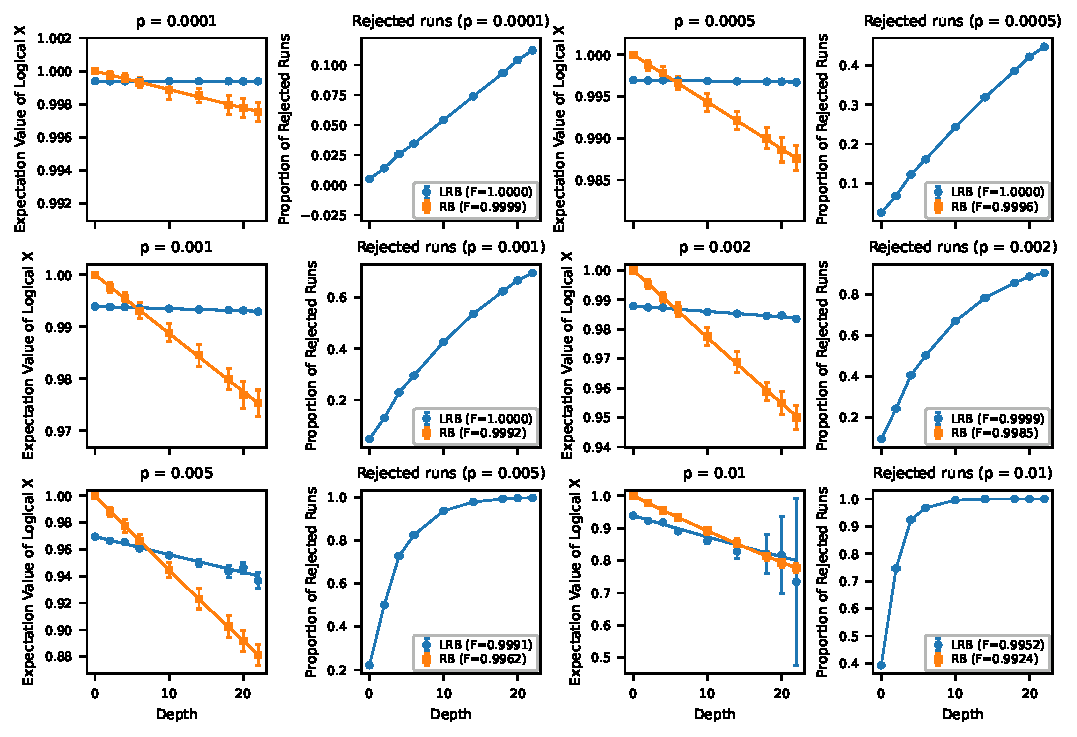
\includegraphics[width=0.78\textwidth]{figures/sdim140/si1000-1anc-unif-4-fit.pdf}
  \caption{Uniform-interval postselection with $k = 4$, one-ancilla layout, SI1000 ($\chi^2 = 9.1$ over nine depths at $p = 5\times10^{-3}$). At $p = 5\times10^{-3}$ the fitted error per unit depth is $9.3\times10^{-4}$, and at $p = 10^{-2}$ it is $4.8\times10^{-3}$, against $7.6\times10^{-3}$ for RB.}
  \label{fig:unif4_si1000_1anc}
\end{figure}

\begin{figure}[H]
  \centering
  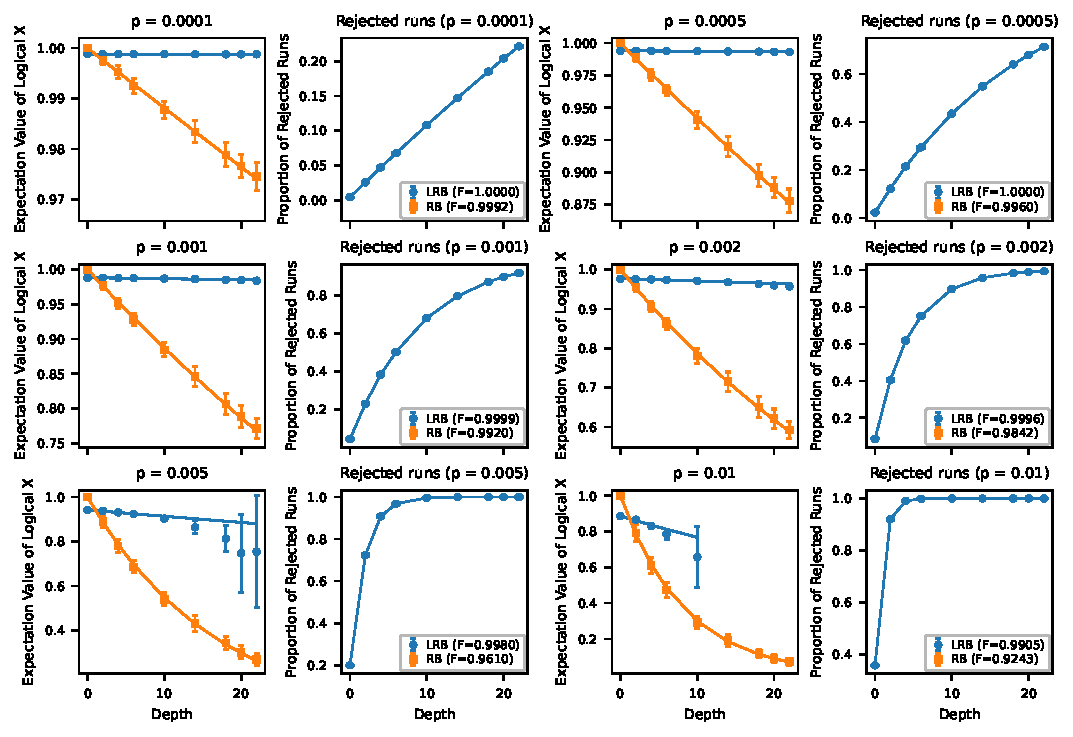
\includegraphics[width=0.78\textwidth]{figures/sdim140/sd6-1anc-unif-2-fit.pdf}
  \caption{Uniform-interval postselection with $k = 2$, one-ancilla layout, SD6, with RB under SD6 ($\chi^2 = 7.5$ over nine depths at $p = 5\times10^{-3}$). At $p = 10^{-2}$ the LRB-D fit uses five depths and gives an error per unit depth of $9.5\times10^{-3}$, against $7.6\times10^{-2}$ for RB.}
  \label{fig:unif2_sd6_1anc}
\end{figure}

\begin{figure}[H]
  \centering
  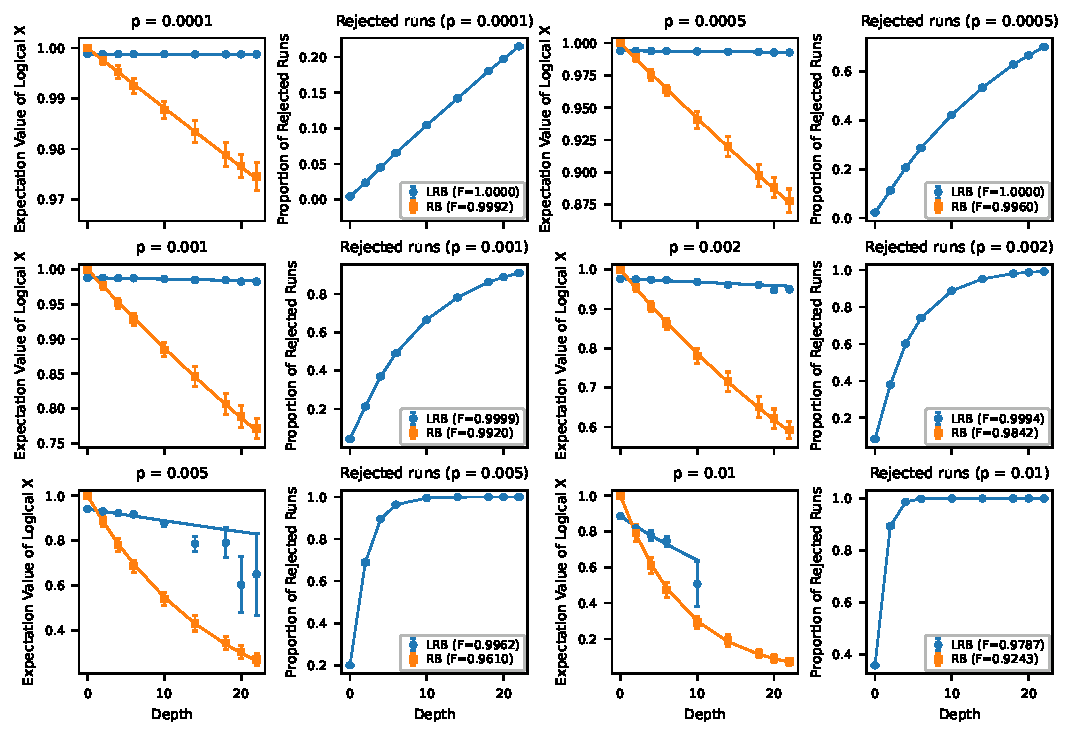
\includegraphics[width=0.78\textwidth]{figures/sdim140/sd6-1anc-unif-3-fit.pdf}
  \caption{Uniform-interval postselection with $k = 3$, one-ancilla layout, SD6 ($\chi^2 = 14.8$ over nine depths at $p = 5\times10^{-3}$). At $p = 10^{-2}$ the LRB-D fit uses five depths and gives an error per unit depth of $2.1\times10^{-2}$.}
  \label{fig:unif3_sd6_1anc}
\end{figure}

\begin{figure}[H]
  \centering
  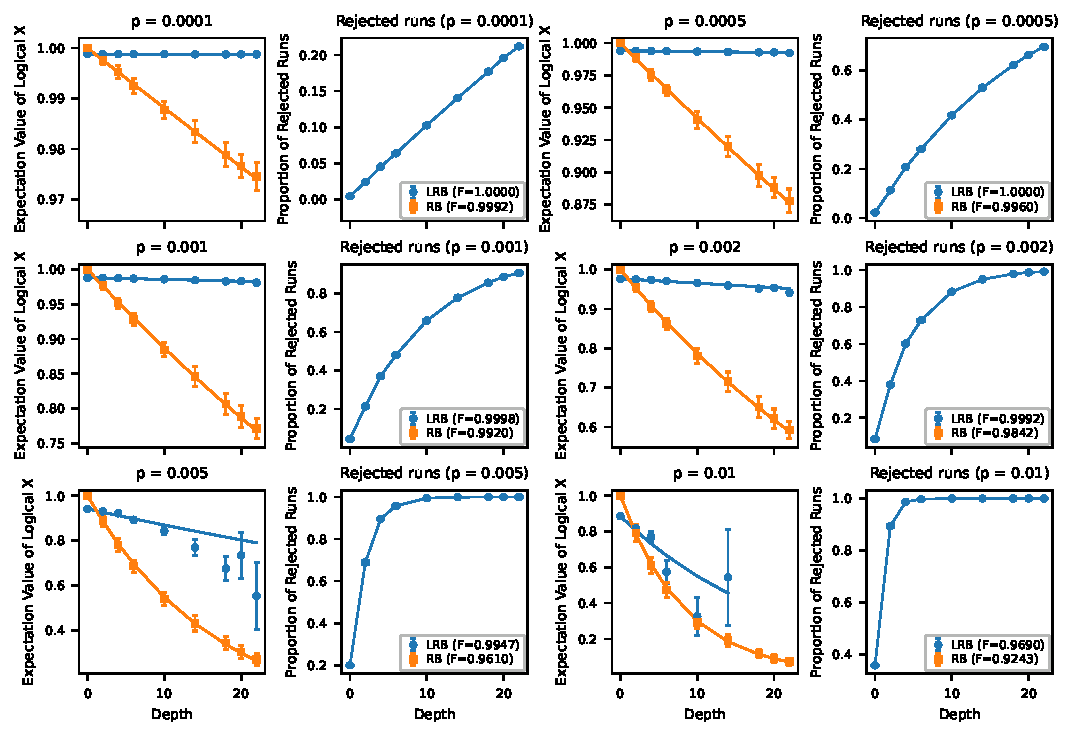
\includegraphics[width=0.78\textwidth]{figures/sdim140/sd6-1anc-unif-4-fit.pdf}
  \caption{Uniform-interval postselection with $k = 4$, one-ancilla layout, SD6 ($\chi^2 = 24.8$ over nine depths at $p = 5\times10^{-3}$). At $p = 10^{-2}$ the LRB-D fit uses six depths and gives an error per unit depth of $3.1\times10^{-2}$. Points that rest on a few accepted shots per sequence scatter upward (\autoref{sub:interval_results}).}
  \label{fig:unif4_sd6_1anc}
\end{figure}

\subsection{Two-Ancilla Layout}

\begin{figure}[H]
  \centering
  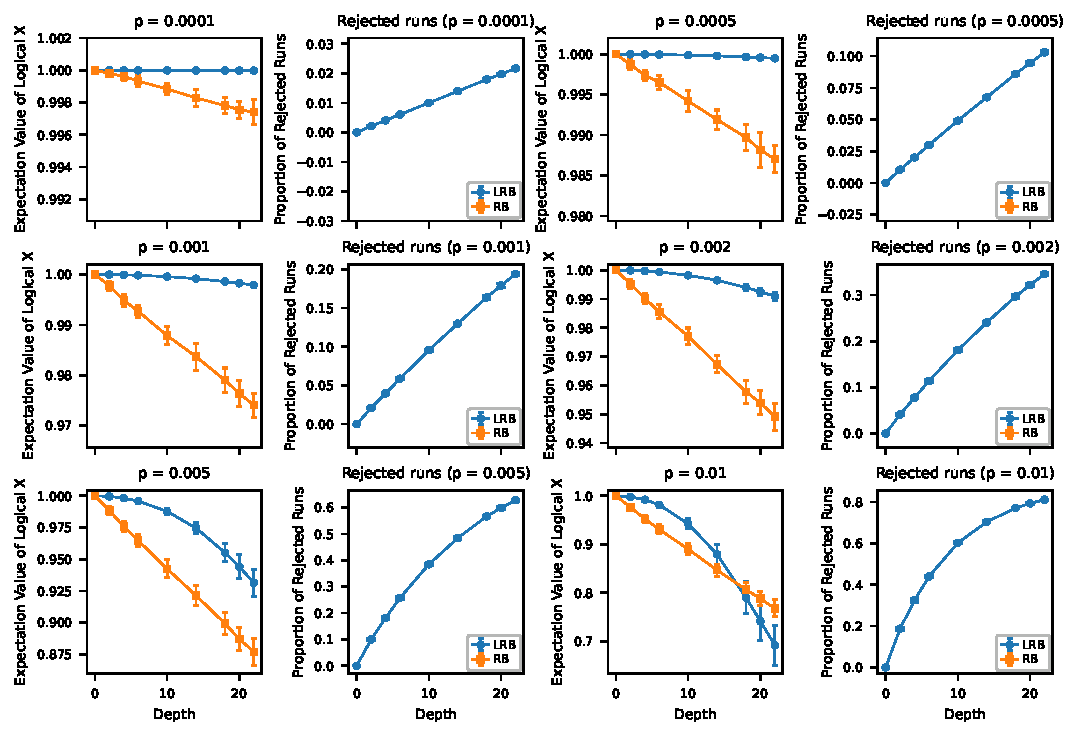
\includegraphics[width=0.78\textwidth]{figures/sdim140/si1000-2anc-const-0-nofit.pdf}
  \caption{Terminal postselection (const-0), two-ancilla layout, SI1000. Without check rounds the two layouts run the same data circuits, and the ancillas only idle, so the traces agree with \autoref{fig:const0_si1000_1anc} up to the independent draw of the 30 sequences. At $p = 5\times10^{-3}$ and $m = 22$, for example, $\langle \bar{X} \rangle = 0.931$ and the rejected fraction is $0.628$, against $0.935$ and $0.622$ for one ancilla.}
  \label{fig:const0_si1000_2anc}
\end{figure}

\begin{figure}[H]
  \centering
  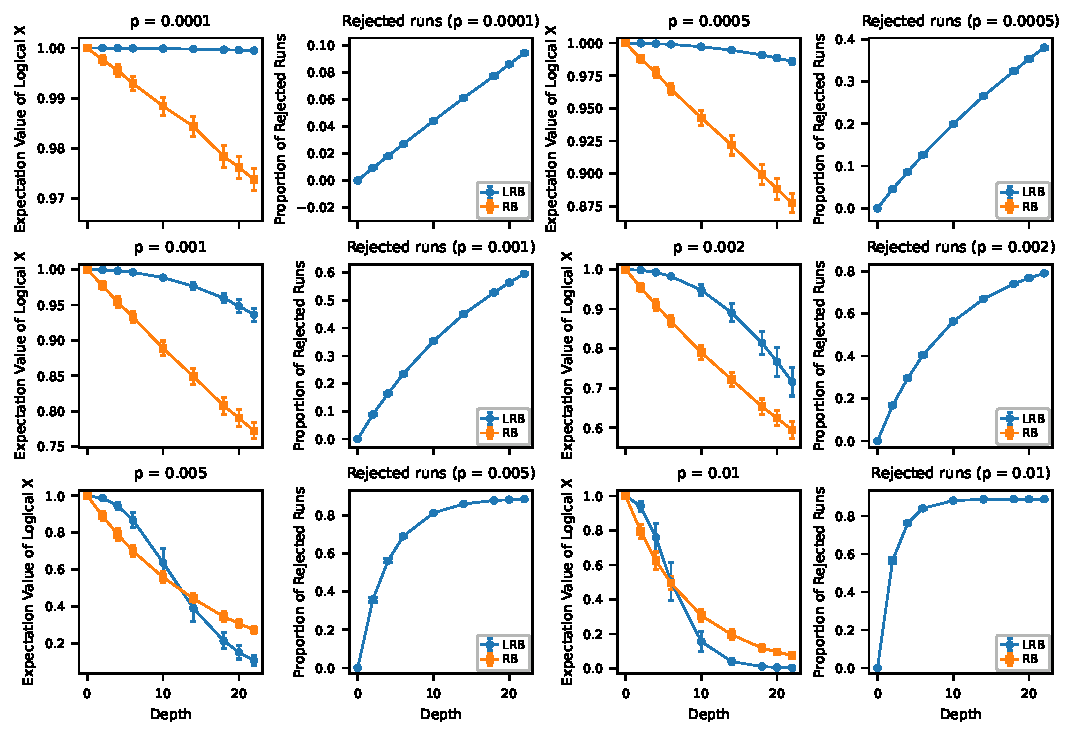
\includegraphics[width=0.78\textwidth]{figures/sdim140/sd6-2anc-const-0-nofit.pdf}
  \caption{Terminal postselection (const-0), two-ancilla layout, SD6. As in \autoref{fig:const0_sd6_1anc}, the rejected fraction approaches $8/9$ (0.8888 at $p = 10^{-2}$ and $m = 22$).}
  \label{fig:const0_sd6_2anc}
\end{figure}

\begin{figure}[H]
  \centering
  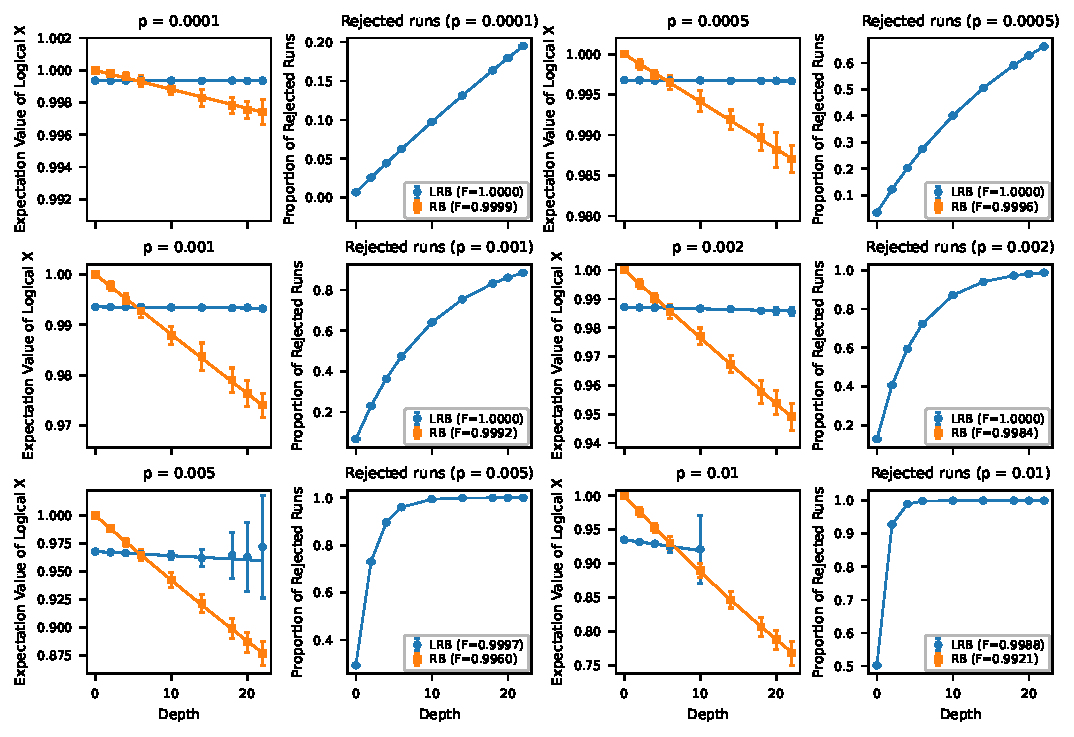
\includegraphics[width=0.78\textwidth]{figures/sdim140/si1000-2anc-unif-1-fit.pdf}
  \caption{Uniform-interval postselection with $k = 1$, two-ancilla layout, SI1000. At $p = 5\times10^{-3}$ the relay raises the rejected fraction at $m = 0$ from 22\% to 29\%, while the fitted error per unit depth stays close to the one-ancilla value ($2.5\times10^{-4}$ against $2.3\times10^{-4}$).}
  \label{fig:unif1_si1000_2anc}
\end{figure}

\begin{figure}[H]
  \centering
  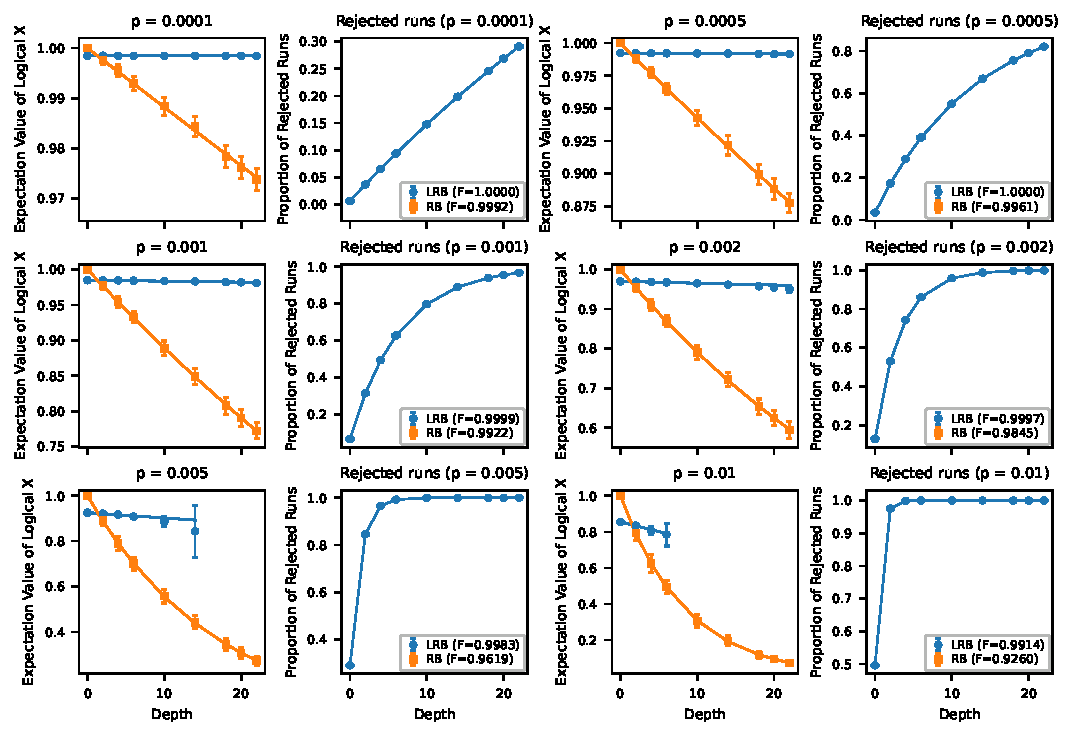
\includegraphics[width=0.78\textwidth]{figures/sdim140/sd6-2anc-unif-1-fit.pdf}
  \caption{Uniform-interval postselection with $k = 1$, two-ancilla layout, SD6. At $p = 5\times10^{-3}$ the rejected fraction at $m = 0$ is 29\% (20\% with one ancilla), the accepted $\langle \bar{X} \rangle$ at $m = 0$ is $0.926$ ($0.941$), and the fitted error per unit depth is $1.7\times10^{-3}$ ($1.4\times10^{-3}$), from a fit over six depths.}
  \label{fig:unif1_sd6_2anc}
\end{figure}

\begin{figure}[H]
  \centering
  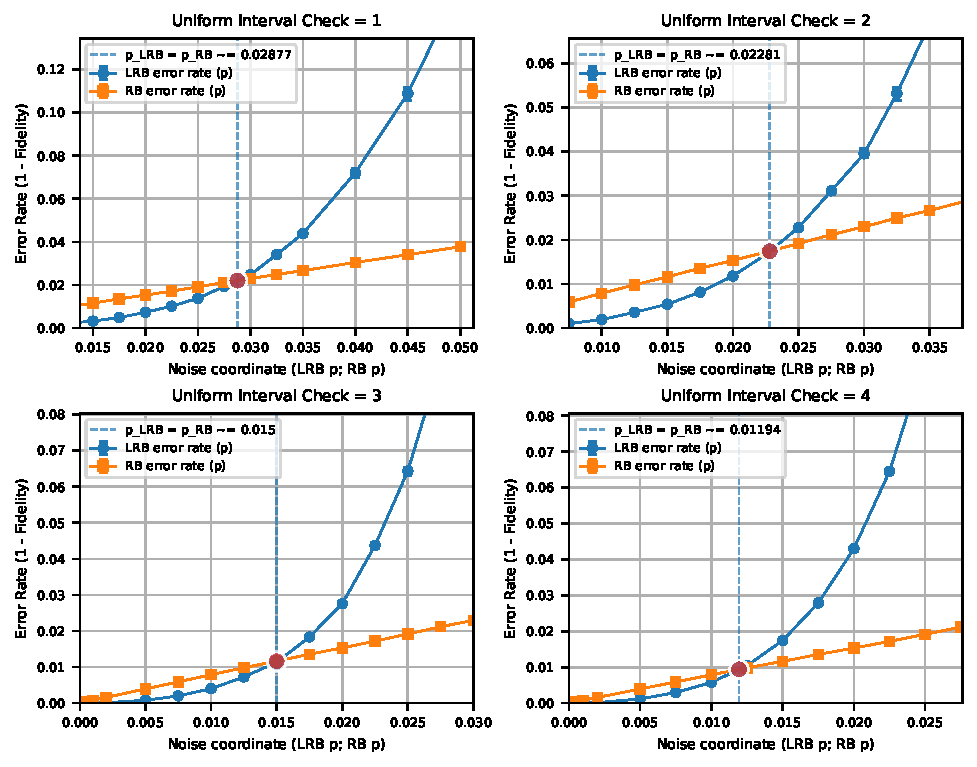
\includegraphics[width=0.85\textwidth]{figures/sdim140/si1000-2anc-threshold-grid.pdf}
  \caption{Pseudo-threshold construction, two-ancilla layout, SI1000, with curves as in \autoref{fig:threshold_grid_si1000_1anc}. Points at $p < 0.015$ come from the production run, and points at $p \ge 0.015$ from the high-$p$ extension, fitted for $k = 1$ over three to six of its depths and for $k \ge 2$ over three or four of its even depths $0, 2, 4$ and $6$ (\autoref{sub:results_setup}). The markers are genuine crossings at $p^\star(k) = 0.0288$, $0.0228$, $0.0150$ and $0.0119$ for $k = 1$ to $4$. For $k = 3$ the LRB-D and RB errors agree within the tolerance at the extension grid point $0.015$ ($0.0113$ against $0.0116$), and the marker sits there. The sign change of their difference lies at $0.0152$. The $k = 1$, $2$ and $3$ crossings lie between extension points, and the $k = 4$ crossing lies between the production points $0.01$ and $0.0125$. The fits that bracket $p^\star(1)$ use five depths ($m \le 4$), those that bracket $p^\star(2)$ and $p^\star(3)$ use four, and those that bracket $p^\star(4)$ use eight and six.}
  \label{fig:threshold_grid_si1000_2anc}
\end{figure}

\begin{figure}[H]
  \centering
  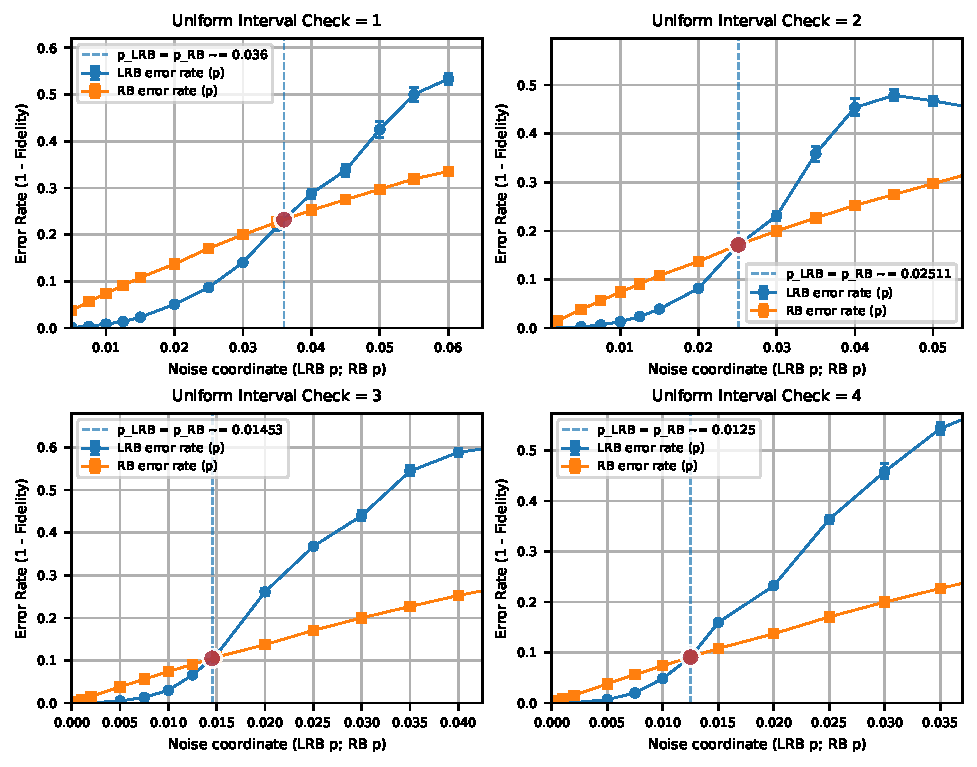
\includegraphics[width=0.85\textwidth]{figures/sdim140/sd6-2anc-threshold-grid.pdf}
  \caption{Pseudo-threshold construction, two-ancilla layout, SD6, with curves as in \autoref{fig:threshold_grid_sd6_1anc}. Points at $p < 0.025$ come from the production run, and points at $p \ge 0.025$ from the high-$p$ extension. There the $k = 1$ fits use those extension depths at which every sequence keeps at least one shot, two to four depths with $m \le 3$, and the $k \ge 2$ fits use two to four of the even depths $0, 2, 4$ and $6$ (\autoref{sub:results_setup}). The markers are genuine crossings at $p^\star(k) = 0.0360$, $0.0251$, $0.0145$ and $0.0125$ for $k = 1$ to $4$. For $k = 4$ the LRB-D and RB errors agree within the tolerance at the production grid point $0.0125$, and the marker sits there. The $k = 1$ and $2$ crossings lie between extension points. For $k = 2$ the fits rest on two depths from $p = 0.045$ on, and above that point the fitted LRB-D error falls slightly.}
  \label{fig:threshold_grid_sd6_2anc}
\end{figure}


\section{Representation Theory}\label{sec:rep-theory}

\subsection{Group Modules and Irreducible Representations}

The aim of this section is to serve as a review of the basics of representation theory.
This will not be an exhaustive review by any means.
For a more thorough mathematical treatment of the representation of finite groups we direct the reader to \cite{sagan2001symmetric}.

Let $G$ denote a finite group. We will denote the identity element of $G$ by $e$ to avoid confusion. 
A $G$-module is a finite dimensional vector space $V$ equipped with a group action $\cdot : G \times V \to V$ satisfying 
\begin{enumerate}
    \item \textbf{(Identity)} For all vectors $\ket{v} \in V$, the equality $e \cdot \ket{v} = \ket{v}$ is satisfied.
    \item \textbf{(Linearity)} For all linear combinations $\alpha \ket{v} + \beta \ket{w}$ and all group elements $g \in G$, the equality $g \cdot (\alpha \ket{v}+\beta\ket{w}) = \alpha (g\cdot \ket{v}) + \beta (g \cdot \ket{w})$ is satisfied.
    \item \textbf{(Compatibility)} For all group elements $g,h \in G$ and vectors $\ket{v} \in V$, the equality $(gh) \cdot \ket{v} = g\cdot (h \cdot \ket{v})$ is satisfied.
\end{enumerate}
The linearity axiom implies the existence of a map $\pi: G \to \mathrm{End}(V)$ mapping the group element $g$ to the linear endomorphism $\ket{v} \mapsto g\cdot \ket{v}$. 
The identity and compatibility axioms imply that $\pi$ is actually a group homomorphism. 

\begin{lemma}
    We call a group homomorphism $\pi : G \to \mathrm{End}(V)$ a representation of $G$. If $\pi: G \to \mathrm{End}(V)$ is a representation, then $V$ is a $G$-module under 
    \begin{align}
        g \cdot \ket{v} = \pi(g)\ket{v}.
    \end{align}
    Moreover, if $V$ is a $G$-module, then the map $\pi(g)(\ket{v}) = g\cdot \ket{v}$ is a representation of $G$.
\end{lemma}
In light of this result, it is somewhat standard to conflate representation of $G$ and $G$-modules. 
As with all linear maps, representations are typically described by how each element of $G$ acts on each basis vector of $V$.
% Alternatively, one can describe a representation by first describing how the group $G$ acts on some set $X$ and then extending the action to the free vector space $\mathbb{C}[X]$ by linearity.

Sometimes, a representation can be reduced to a direct sum of smaller representations in the sense that 
\begin{align}
    \pi(g) = \pi_0(g) \oplus \pi_1(g) \oplus \dots \oplus \pi_k(g)
\end{align}
for each $\pi_i$ a representation.
In this case, we write $\pi = \pi_0 \oplus \dots \oplus \pi_k$.
This corresponds to a decomposition of $G$-modules $V = V_0 \oplus \dots \oplus V_k$ where each $V_i$ is a $G$-module.
If no such decomposition exists, then we call the representation (or $G$-module) irreducible.
Irreducible representations are typically referred to by the abbreviation ``irrep''.

\begin{theorem}[Maschke's Theorem \cite{sagan2001symmetric} Theorem 1.5.3] \label{thm:maschkes-theorem}
    Every representation $\pi : G \to \mathrm{End}(V)$ decomposes into a direct sum
    \begin{align}
        \pi \cong m_0 \pi_0 \oplus m_1 \pi_1 \oplus \dots \oplus m_k \pi_k
    \end{align}
    where $\pi_i$ and $\pi_j$ are distinct irreducible representations of $G$. Here $m_i \pi_i \cong \bigoplus_{j=0}^{m_i - 1} \pi_i$.

    Similarly, if $V$ is a finite dimensional $G$-module, then 
    \begin{align}
        V = m_0 V_0 \oplus \dots \oplus m_k V_k
    \end{align}
    where $V_i$ and $V_j$ are distinct irreducible $G$-modules.
\end{theorem}
Maschke's theorem requires two caveats.
Firstly, the characteristic of the underlying field must not divide $|G|$, which holds over $\mathbb{C}$.
Secondly, it must be possible to average over the group, so an analog of Maschke's theorem holds for compact Lie groups.
The form of Schur's lemma used below additionally requires an algebraically closed field such as $\mathbb{C}$.

\subsubsection{Schur's Lemma}

Suppose that $V$ is a $G$-module. 
We let $\mathrm{End}_G(V)$ denote all of the elements $T \in \mathrm{End}(V)$ such that for all $g \in G$
\begin{align}
    T \pi(g) = \pi(g)T.
\end{align}
Such elements $T$ are said to be invariant under the action of $G$ or $G$-linear.
This condition ends up being rather stringent.

\begin{lemma}[Schur's Lemma \cite{sagan2001symmetric} Theorem 1.6.5]\label{lem:schurs-lemma}
    Let $V$ and $W$ be $G$-modules and let $\pi_V$ and $\pi_W$ be the associated representations.
    We define $\mathrm{Hom}_G(V, W)$ by $T \in \mathrm{Hom}_G(V, W)$ if for all $g \in G$
    \begin{align}
        T \pi_V(g) = \pi_W(g) T.
    \end{align}
    If $V$ and $W$ are irreducible, then exactly one of the following holds.
    \begin{enumerate}
        \item The $G$-modules $V$ and $W$ are not isomorphic and $\mathrm{Hom}_G(V,W) = 0$.
        \item The $G$-modules $V$ and $W$ are isomorphic and $\mathrm{Hom}_G(V,W) \cong \mathbb{C}$ in the sense that $\mathrm{End}_G(V) = \{ \lambda I_V \mid \lambda \in \mathbb{C} \}$.
    \end{enumerate}
\end{lemma}

\begin{cor}[\cite{sagan2001symmetric} Theorem 1.7.9]
    Let $V$ be a $G$-module such that
    \begin{align}
        V = m_0 V_0 \oplus \dots \oplus m_k V_k
    \end{align}
    with $V_i$ and $V_j$ distinct irreducible modules.
    Let $d_i$ be the dimension of $V_i$.
    Then the following hold.
    \begin{enumerate}
        \item The dimension of $V$ is given by $\mathrm{dim}(V) = m_0 d_0 + \dots + m_k d_k$.
        \item \label{item:artin-wedderburn} The endomorphism algebra of $V$ is isomorphic to the direct sum
        \begin{align}
            \mathrm{End}_G(V) \cong \bigoplus_{i = 0}^k \mathrm{End}(\mathbb{C}^{m_i}).
        \end{align}
        \item The endomorphism algebra $\mathrm{End}_G(V)$ has dimension $m_0^2 + m_1^2 + \dots + m_k^2$.
    \end{enumerate}
\end{cor}

\begin{proof}
    We will only include a proof of \Cref{item:artin-wedderburn} as it is the most important.
    From the decomposition of $V$, we get the equality
    \begin{align}
        \mathrm{End}_G(V) \cong \bigoplus_{i,j = 0}^k \mathrm{Hom}_G(m_iV_i,m_jV_j).
    \end{align}
    The elements of $\mathrm{Hom}_G(m_i V_i, m_j V_j)$ can be thought of as $m_i \times m_j$ matrices whose entries are in $\mathrm{Hom}_G(V_i, V_j)$. 
    However, if $i \neq j$, then by Schur's lemma we know that $\mathrm{Hom}_G(V_i, V_j)$ only contains the zero map. 
    Thus, all of the terms in the direct sum for $i \neq j$ are zero and can be ignored. 
    When $i = j$, the elements of $\mathrm{Hom}_G(V_i,V_i) = \mathrm{End}_G(V_i)$ are all multiples of the identity map. 
    So, the elements $g_i \in \mathrm{End}_G(m_iV_i)$ can be written in the form
    \begin{align}
        g_i = M_i \otimes I_{V_i},
    \end{align}
    where $M_i \in \mathrm{End}(\mathbb{C}^{m_i})$ is an $m_i \times m_i$ matrix with complex entries. 
    % Moreover, any such matrix $M_i$ defines an element $g_i = M_i \otimes I_{V_i} \in \mathrm{End}_G(m_i V_i)$.
    A routine argument shows $\mathrm{End}_G(m_iV_i)$ is isomorphic to the matrix algebra $\mathrm{End}(\mathbb{C}^{m_i})$ under the map $g_i \mapsto M_i$.
    Finally, we conclude that $\mathrm{End}_G(V) \cong \bigoplus_{i = 0}^k \mathrm{End}_G(m_i V_i)$ and hence
    \begin{align}
        \mathrm{End}_G(V) \cong \bigoplus_{i=0}^k \mathrm{End}(\mathbb{C}^{m_i}).
    \end{align}
\end{proof}

Concretely, Schur's lemma and its corollary impose a relatively stringent structure on the elements of $\mathrm{End}_G(V)$. 
For our purposes the most important property is that if $T \in \mathrm{End}_G(V)$ and $\ket{v} \in m_i V_i$ is supported entirely in copies of the $V_i$ module, then $T\ket{v} \in m_i V_i$ is also supported entirely in copies of $V_i$. 
The following result guarantees that the twirled error channel that we aim to study is invariant under the action of the Clifford group.

\begin{lemma}[Twirling] \label{lem:twirling}
    Suppose $V$ is a finite dimensional $G$-module with associated representation for $G$ finite. Given any $T \in \mathrm{End}(V)$ (notably $T$ need not be $G$-linear), the twirled map
    \begin{align}
        T_G = \frac{1}{|G|} \sum_{g \in G} \pi(g)^{-1} T \pi(g)
    \end{align}
    is an element of $\mathrm{End}_G(V)$.
\end{lemma}

\begin{proof}
    Fix $g \in G$. Conjugating $T_G$ by $\pi(g)$ yields 
    \begin{align}
        \pi(g)^{-1} T_G \pi(g) = \frac{1}{|G|} \sum_{h \in G} \pi(g)^{-1} \pi(h)^{-1} T \pi(h) \pi(g) = \frac{1}{|G|} \sum_{h \in G} \pi(hg)^{-1} T \pi(hg).
    \end{align}
    Since the right coset $Gg$ is equal to $G$, we can reindex the sum to obtain 
    \begin{align}
        \pi(g)^{-1} T_G \pi(g) = \frac{1}{|G|} \sum_{h \in G} \pi(hg)^{-1} T \pi(hg) = \frac{1}{|G|} \sum_{h \in G} \pi(h)^{-1} T \pi(h) = T_G.
    \end{align}
    We conclude that $\pi(g)^{-1} T_G \pi(g) = T_G$ and hence $T_G \pi(g) = \pi(g) T_G$.
\end{proof}

\subsection{Character Theory}

\Cref{item:artin-wedderburn} and \Cref{lem:twirling} show us that in order to fully understand a twirled channel, it is necessary to understand how many copies of each irreducible representation are present in a given representation.
Luckily, if the irreps are understood, then there is an efficient algorithm for computing how many copies of that irrep occur in the decomposition.
This technique comes from a subject called character theory.

\subsubsection{Characters and Conjugacy Classes}

If $\pi : G \to \mathrm{End}(V)$ is a representation, then the character $\chi_\pi : G \to \mathbb{C}$ of $\pi$ is defined by 
\begin{align}
    \chi_\pi(g) = \Tr \pi(g).
\end{align}
By the cyclic property of the trace, characters satisfy the property $\chi_\pi(h g h^{-1}) = \chi_\pi(g)$.
Because of this, characters are constant on the conjugacy classes.
Such a function is called a class function.
Evidently, the space of class functions has dimension equal to the number of conjugacy classes of $G$.
Moreover, the space is equipped with a natural inner product 
\begin{align}
    \langle \chi, \tau \rangle = \frac{1}{|G|} \sum_{g \in G} \chi(g)^* \tau(g).
\end{align}
The following lemma is among the most important results in character theory.

\begin{lemma}[Character Orthogonality \cite{sagan2001symmetric} Theorem 1.9.3] \label{lem:character-orthogonality}
    If $\pi_1$ and $\pi_2$ are irreducible representations of the finite group $G$, then 
    \begin{align}
        \langle \chi_{\pi_1}, \chi_{\pi_2}\rangle = \begin{cases}
            1 & \pi_1 \cong \pi_2, \\
            0 & \text{otherwise}.
        \end{cases}
    \end{align}
\end{lemma}

\begin{cor}[\cite{sagan2001symmetric} Corollary 1.9.4] \label{cor:character-relations}
    Let $\pi : G \to \mathrm{End}(V)$ be a representation and $\pi = m_0 \pi_0 \oplus \dots \oplus m_k \pi_k$ be the decomposition of the representation $\pi$ into irreps. The following hold.
    \begin{enumerate}
        \item The character $\chi_{\pi}$ can be written as $\chi_{\pi} = m_0 \chi_{\pi_0} + m_1 \chi_{\pi_1} + \dots + m_k \chi_{\pi_k}$.
        \item \label{item:irrep-mult-test} The inner product $\langle \chi_{\pi}, \chi_{\pi_i}\rangle = m_i$ for all $0 \leq i \leq k$.
        \item The inner product $\langle \chi_{\pi}, \chi_{\pi} \rangle = m_0^2 + \dots + m_k^2$. In particular this is always an integer.
        \item The representation $\pi$ is irreducible if and only if $\langle \chi_{\pi}, \chi_{\pi} \rangle = 1$.
        \item If $\tau$ is another representation of $G$, then $\pi$ and $\tau$ are isomorphic if and only if $\chi_{\pi}(g) = \chi_{\tau}(g)$ for all $g \in G$.
    \end{enumerate}
\end{cor}

\Cref{lem:character-orthogonality} and \Cref{cor:character-relations} show us two remarkable facts.
Firstly, the irrep characters are orthonormal and thus linearly independent.
Together with the completeness of the irreducible characters, which span the space of class functions \cite{sagan2001symmetric}, this shows that the irrep characters form a basis for that space and, in particular, that there are exactly as many irreps as there are conjugacy classes of $G$.
Secondly, \Cref{item:irrep-mult-test} gives us an efficient method of determining how many copies of a given irrep are present in an arbitrary representation of $G$.

\section{The \texttt{sdim} Simulator and Detector Error Model Sampling}
\label{sec:sdim-dem}

This appendix describes the simulation machinery behind the numerical results of \autoref{sec:results}. All four production runs, the one-ancilla and two-ancilla layouts under SI1000 and under SD6, are sampled through the exact compact $q$-ary detector error model (DEM) of \texttt{sdim} 1.4.0 \cite{sdim}. The physical RB baselines and the four high-$p$ extension runs of \autoref{sub:results_setup}, one per layout and noise model, are sampled in the same way.

\subsection{Qudit stabilizer simulation}

\texttt{sdim} \cite{sdim} is a tableau-based stabilizer simulator for prime-dimensional qudits. It generalizes the binary tableau formalism of \cite{Aaronson2004} to arithmetic over $\mathbb{Z}_q$, representing stabilizer generators as Weyl operators $\omega^c X^{\mathbf{a}} Z^{\mathbf{b}}$ with exponent vectors $\mathbf{a}, \mathbf{b} \in \mathbb{Z}_q^n$ \cite{Gottesman1999,Hostens2005}. Clifford gates act on the tableau by linear updates of these exponent vectors, and computational or Fourier-basis measurements are handled by the qudit analog of the usual stabilizer measurement rules. All circuits in this work use $q=3$.

Noise is included through parameterized Pauli channels, inserted as explicit noise operations in the circuit. The single-qutrit operation carries a channel tag and a probability. The depolarizing tag applies a uniformly random non-identity $X^a Z^b$ with the stated probability, the shift tag applies $X^a$ with $a$ uniform on $\{1,2\}$, and the phase tag applies $Z^b$ with $b$ uniform on $\{1,2\}$. The two-qutrit operation applies a uniformly random non-identity two-qutrit Pauli. The circuit-level models of \autoref{sub:noise_models} use the depolarizing tag for every DEP1 location, the two-qutrit operation for every DEP2 location, and the shift tag for every reset and measurement flip. The probability of each operation is the swept parameter $p$ times its multiplier in \autoref{tab:circuit-noise}. Every $X$-basis readout in our circuits is compiled as $H^{-1}$ followed by a computational-basis measurement, so every measurement flip is a shift flip and the phase tag does not occur.

Rather than rerunning the tableau algorithm shot by shot, \texttt{sdim} samples in the Pauli frame picture. A single noiseless reference shot is simulated with the full tableau algorithm. For every additional shot, only a Pauli frame, one pair of exponents $(a_i, b_i)$ per qutrit, is propagated through the Clifford circuit. Noise operations update the frame stochastically, and each computational-basis measurement returns the reference outcome shifted by the $X$ exponent of the frame on the measured qutrit, modulo three. As in Stim \cite{Gidney2021Stim}, the frame simulator draws a random $Z$ component of the frame at the start of the circuit and after every computational-basis measurement and reset, which accounts for measurement outcomes that are random in the reference shot. This separates the polynomially expensive stabilizer computation, done once, from the cheap per-shot frame propagation.

\subsection{Detectors and logical observables}

A detector is a linear combination of measurement records, $D = \sum_i c_i m_i \bmod 3$ with integer coefficients $c_i$, chosen so that $D$ takes a fixed known value on every noiseless execution of the circuit. A logical observable is the same kind of expression evaluated on the logical readout. In our mirror circuits it is also deterministic without noise, and a deviation from its noiseless value is a logical error. This is the qudit generalization of the detector formalism introduced by Stim for qubit circuits \cite{Gidney2021Stim}, with sums modulo two replaced by sums modulo three and with coefficients $\pm 1$ to account for inverted stabilizer components.

An LRB-D circuit of depth $m$ contains $m+1$ check rounds. As in \autoref{sub:lrb_d}, round $t \le m$ follows the forward Clifford $\bar C_t$, and round $m+1$ is the final round after the mirror inverse. We declare one detector per ancilla readout per round, labeled by the round and the ancilla wire. The labels in our circuit files use the zero-based round index $t - 1$. Each ancilla is reset just before its round, and without noise the data stay in the code space, so every syndrome readout is zero and every relay returns to $\ket{0}$. Each detector is therefore the readout itself, with coefficient one. In the one-ancilla layout the ancillas on wires 5 to 8 carry the syndromes of $G_1$ to $G_4$, which gives four detectors per round and $4(m+1)$ in total. In the two-ancilla layout of \autoref{sub:ancilla_layouts}, wires 5 to 8 again carry the four syndromes, and the relay ancillas on wires 9 and 10, which serve the boundary stabilizers $G_1$ and $G_4$, add two detectors per round. This gives six detectors per round and $6(m+1)$ in total, so the depth-22 circuits carry 92 and 138 detectors. A round passes when all of its detectors vanish, so a nonzero relay readout rejects the round even when the reconstructed syndrome reads zero. The logical observable is $x_0 + x_3 \bmod 3$ on the terminal $X$-basis readouts $x_0$ and $x_3$ of qutrits $q_0$ and $q_3$, matching $\bar{X} = X_0 \otimes X_3$.

The circuits for terminal postselection (const-0) contain no check rounds. All five data qutrits are read out ideally in the $X$ basis at the end, with outcomes $x_0, \dots, x_4$, and the two $X$-type stabilizers are declared as detectors with the coefficient patterns $x_0 + x_1 - x_2$ and $x_3 - x_1 - x_4$, mirroring $G_3$ and $G_4$. The $Z$-type stabilizers are not checked, since $X$-basis outcomes carry no information about them. The logical observable is again $x_0 + x_3$. Physical RB circuits contain no detectors and one logical observable, the terminal readout of the single qutrit.

A postselection schedule is not part of the circuit. It is a rule that selects which rounds must pass, and it is applied to the sampled detector values. Uniform-interval postselection with interval $k$ requires the rounds after the forward Cliffords $\bar C_k, \bar C_{2k}, \dots$ with index at most $m$, together with the final round. The production runs also record constant-number schedules const-$n$ for $n = 1, \dots, 22$. Each requires the final round and, when $n \le m$, the $n-1$ rounds after $\bar C_{j\lfloor m/n \rfloor}$ for $j = 1, \dots, n-1$. With const-0 and $k = 1, \dots, 22$ this makes 45 schedules. The 44 schedules other than const-0 are evaluated on the same shots of the same LRB-D circuits. One compiled model per circuit therefore serves all of them, and estimates for different schedules at the same $p$, sequence and depth are statistically correlated.

\subsection{The compact detector error model}

A detector error model is a list of independent error mechanisms, each with a firing probability and its effect on every detector and logical observable. The construction rests on linearity. Write a Pauli fault on the $n \in \{1,2\}$ qutrits of one noise operation, up to phase, as an exponent vector $e = (a_1, b_1, \dots, a_n, b_n) \in \mathbb{Z}_3^{2n}$. The fault propagates through the remaining Clifford circuit to a Pauli frame whose exponents depend linearly on $e$, and detectors and observables are linear in the measurement records. The fault therefore shifts the vector of all detector and observable values by
\begin{equation}
    \Delta(e) = \sum_{j=1}^{n} \left( a_j\, r^X_j + b_j\, r^Z_j \right) \bmod 3,
    \label{eq:dem-shift}
\end{equation}
where $r^X_j$ and $r^Z_j$ are the responses to a unit $X$ or $Z$ fault on qutrit $j$, placed right after the operation. \texttt{sdim} computes all unit responses in one backward sweep over the circuit, as Stim does \cite{Gidney2021Stim}. For every qutrit it keeps the linear map from the $X$ and $Z$ components of its frame to the detectors and observables, updates these maps with the transpose of each gate's frame rule, and reads off the responses at each noise operation.

The model is built by \texttt{DetectorErrorModel.from\_circuit}. Every noise operation with nonzero probability and at least one nonzero unit response becomes one mechanism. The generators $g_j$ of the mechanism are its nonzero unit responses, at most two for a DEP1 location, one for a shift flip, and at most four for a DEP2 location. When the mechanism fires, it adds $\sum_j c_j g_j$ to the detector and observable values, with the $c_j$ independent and uniform on $\mathbb{Z}_3$, zero included. A depolarizing operation with probability $p_\ell$ on $n$ qutrits is exactly such a mechanism. Applying a uniformly random non-identity Pauli with probability $p_\ell$ is the same channel as applying a uniformly random Pauli, identity included, with probability
\begin{equation}
    \pi_\ell = \frac{9^n}{9^n - 1}\, p_\ell ,
\end{equation}
because the second form draws the identity with probability $9^{-n}$. This gives $\pi_\ell = 9p_\ell/8$ for DEP1 and $\pi_\ell = 81p_\ell/80$ for DEP2, and the same argument gives $\pi_\ell = 3p_\ell/2$ for a shift flip. A uniformly random $e$ has independent uniform components, so by \eqref{eq:dem-shift} its shift is $\sum_j c_j g_j$ with independent uniform $c_j$. This holds even when the generators are linearly dependent. One mechanism per noise operation therefore reproduces the effect of the channel on all detectors and observables jointly, including the correlations between its Pauli components. Splitting a DEP1 location into eight independent events, one per non-identity Pauli, would only approximate the channel, because a depolarizing channel applies exactly one of its Paulis, so its outcomes are disjoint rather than independent.

Two mechanisms with one generator each act on the same line of detector space when one generator is a nonzero multiple of the other. \texttt{sdim} merges all mechanisms on one line into a single mechanism with $1 - \pi = \prod_i (1 - \pi_i)$. The merge is exact, because a uniformly random multiple of a vector plus any independent multiple of the same vector is again a uniformly random multiple. The binary XOR rule does not carry over to $q = 3$, since a shift applied twice does not cancel. Mechanisms with two or more generators are kept as they are. Before building the model, \texttt{sdim} checks that every detector and observable is linear in its records, has no constant term, and is deterministic in the noiseless circuit. The determinism check places a unit $Z$ fault at every point where the frame simulator draws a random $Z$ component and requires that none of them reaches a detector or observable.

Noise operations whose faults reach no detector or observable are dropped. In the LRB-D circuits these are almost all DEP1 locations on ancillas before a reset, whose effect the reset erases, or after the readout of the final round. In the const-0 circuits they are the idle locations of the ancillas, which are never measured. The size of the model does not depend on $p$ for $p > 0$. Across the 30 sequences and both noise models, the depth-22 one-ancilla LRB-D circuits contain 3701 to 4465 noise operations and compile to 2199 to 2603 mechanisms on 92 detectors and one observable. The corresponding two-ancilla circuits contain 5137 to 6039 noise operations and compile to 2618 to 3006 mechanisms on 138 detectors. The const-0 circuits of the same depth compile to 421 to 976 mechanisms on two detectors, and the physical RB circuits to 54 to 178 mechanisms on one observable.

\subsection{Sampling and exactness}

Sampling the compiled model is elementary. For each shot, every mechanism fires independently with its probability $\pi_\ell$. When a mechanism fires, its coefficients $c_j$ are drawn and $\sum_j c_j g_j$ is added to the detector and observable values modulo three. The sampler avoids visiting every mechanism in every shot. It groups the mechanisms into bins of similar probability, jumps to the next candidate firing in a bin with a geometric skip, and keeps a candidate with probability $\pi_\ell / \pi_{\max}$, where $\pi_{\max}$ is the largest probability in its bin. Shots are drawn in blocks of 256, each block with its own pseudo-random stream, so the samples do not depend on the number of threads.

The sampled values are shifts relative to the noiseless reference shot. Our pipeline computes that shot once per circuit by tableau simulation of the circuit with all noise removed, evaluates every detector and observable on it, and adds these reference values to the sampled shifts. The reference value of every detector is zero, as expected for checks of a code state read out on freshly reset ancillas. A shot passes a check round when all detectors of that round vanish, and its logical outcome is the reference value of the observable plus the sampled shift.

Our noise models consist entirely of Pauli channels acting inside Clifford circuits, and different noise operations are independent. Faults compose additively in the frame picture, so the joint shift of all detectors and observables is a sum of independent contributions, one per noise operation, each distributed as its mechanism. The model therefore reproduces exactly the joint distribution of detector and logical events that direct frame simulation would produce. Nothing is approximated at any $p$ of our grid. The largest local probability, the SI1000 measurement flip $5p = 0.25$ at $p = 0.05$, lies below the fully mixing value $2/3$ of a shift flip, up to which the subgroup form above holds.

We also compared the DEM sampler with direct frame simulation. For both layouts and both noise models, we generate depth-2 LRB-D, const-0 and physical RB circuits with the production circuit generator at $p = 0.01$ and sample $4 \times 10^4$ shots with each backend. The pass rate of every check round, the rate of shots that pass every round and return the noiseless logical outcome, and the rate of correct logical outcomes agree between the backends within five standard errors of a two-proportion test. At $p = 0$, every check passes and the logical outcome is constant with both backends.

What the DEM changes is the cost profile. After a one-time compilation per circuit, the per-shot work is proportional to the expected number of firing mechanisms, $\sum_\ell \pi_\ell$, and not to the size of the stabilizer computation. This is what made $10^6$ LRB-D shots per sequence and depth affordable on the full grid of 15 noise strengths, 9 depths and 45 postselection schedules in all four production runs of \autoref{sec:results}.


\section{Generating the Single-Qutrit Clifford Group}
\label{sec:clifford-gen}

Both the physical RB baseline and the LRB-D protocol draw every Clifford uniformly from the single-qutrit Clifford group. We therefore need an explicit catalog of its elements, a realization of each element as a circuit, and the inverse of each element for the mirror inverse $C_m^{-1}, \dots, C_1^{-1}$, applied in this order. This appendix records how that catalog is constructed and how its elements become circuits.

Modulo global phases, the single-qutrit Clifford group $\mathcal{C}_3$ contains $216$ elements. It factors into the qutrit Pauli group and the quotient $\mathcal{C}_3 / \mathcal{P}_3$, which is isomorphic to the symplectic group $Sp(2,\mathbb{Z}_3) = SL(2,\mathbb{Z}_3)$ of order $24$ \cite{Appleby2005,Hostens2005}. Counting phase-free Pauli representatives $X^a Z^b$ with $a,b \in \mathbb{Z}_3$ gives $9$ elements, and $9 \times 24 = 216$. We exploit this factorization and build the group in two stages, first the $24$ coset representatives and then their products with the $9$ Pauli monomials.

\paragraph{Coset representatives from a Cayley graph.}
The quotient $\mathcal{C}_3/\mathcal{P}_3$ is generated by the images of $H$ and $S$. Two Cliffords lie in the same coset exactly when they act in the same way, by conjugation, on the eight non-identity Pauli classes $\{X, Z, XZ, X^2, Z^2, X^2Z, Z^2X, X^2Z^2\}$. This action therefore realizes the quotient faithfully as a permutation group on eight symbols. We perform a breadth-first traversal of the Cayley graph of this group. Starting from the identity, every element of the current level is multiplied on the right by $H$ and then by $S$, and the first time a new element is produced we record its label as the label of its parent extended by the corresponding generator symbol. Because the traversal is breadth-first, each of the $24$ elements receives a minimal-length word in $H$ and $S$, and the traversal terminates once all $24$ are found. The longest of these words has five symbols. In the figure and in the text we write repeated symbols as powers, so for instance $SSHS$ appears as $S^2HS$. The power notation is only a label, and in the circuits every symbol remains a separate gate. The graph explored by this traversal is shown in \autoref{fig:cayley-c3modp3}, with every node carrying the word that the traversal assigned to it.

\begin{figure}[H]
  \centering
  \resizebox{0.92\textwidth}{!}{%
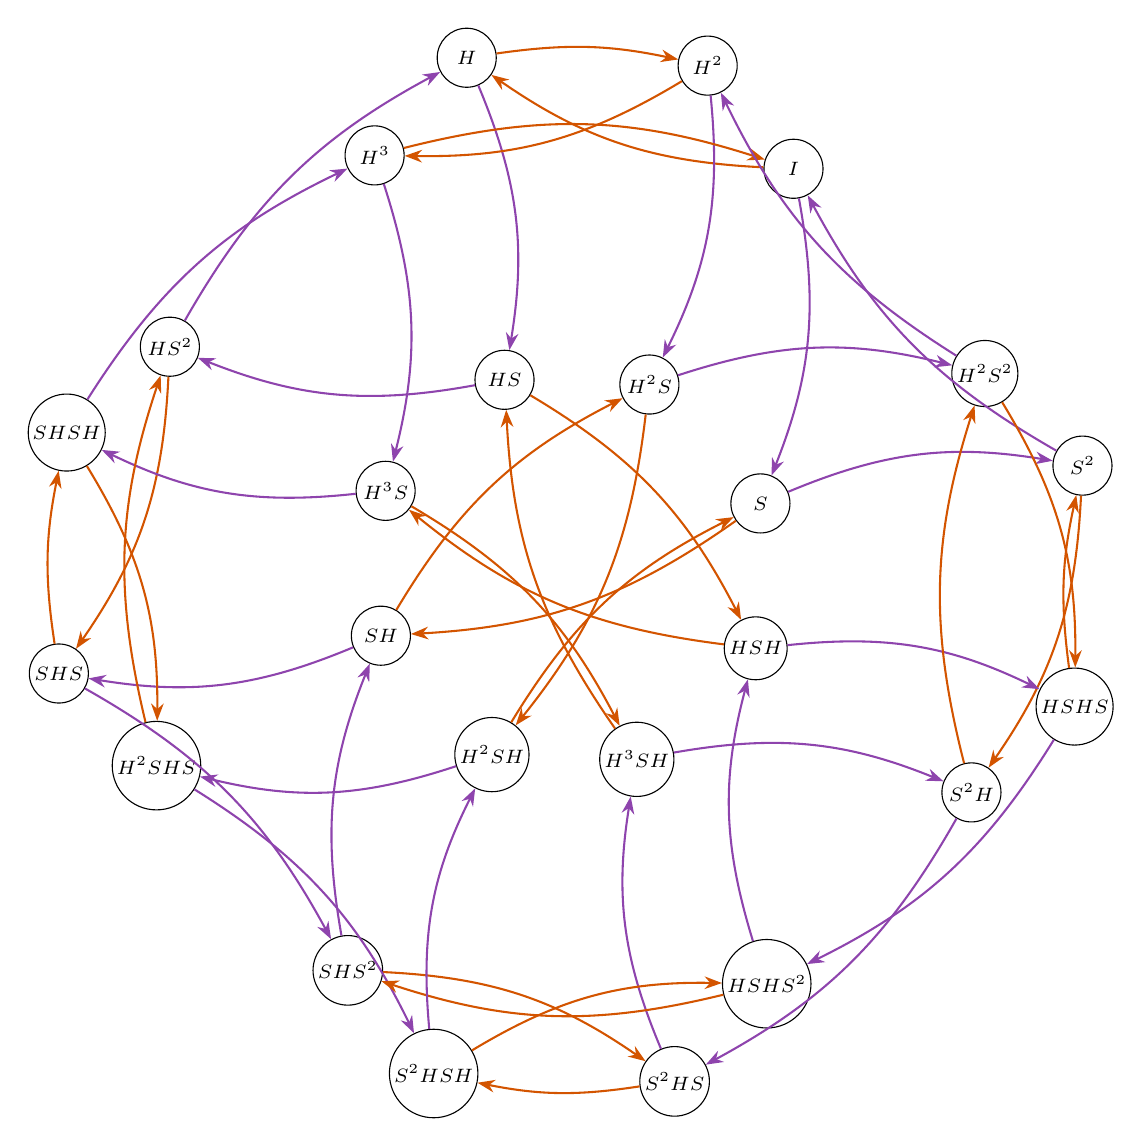
\begin{tikzpicture}[>={Stealth[length=2.2mm,width=1.6mm]},
  cnode/.style={circle,draw=black,fill=white,inner sep=1.1pt,minimum size=7.5mm,font=\scriptsize},
  Hedge/.style={->,HCol,line width=0.75pt},
  Sedge/.style={->,SwapCol,line width=0.75pt}]
  \node[cnode] (n0) at (2.83,5.09) {$I$};
  \node[cnode] (n1) at (-1.32,6.5) {$H$};
  \node[cnode] (n2) at (2.41,0.84) {$S$};
  \node[cnode] (n3) at (1.74,6.4) {$H^2$};
  \node[cnode] (n4) at (-0.84,2.41) {$HS$};
  \node[cnode] (n5) at (-2.41,-0.84) {$SH$};
  \node[cnode] (n6) at (6.5,1.32) {$S^2$};
  \node[cnode] (n7) at (-2.49,5.26) {$H^3$};
  \node[cnode] (n8) at (1.0,2.35) {$H^2S$};
  \node[cnode] (n9) at (2.35,-1.0) {$HSH$};
  \node[cnode] (n10) at (-5.09,2.83) {$HS^2$};
  \node[cnode] (n11) at (-6.5,-1.32) {$SHS$};
  \node[cnode] (n12) at (5.09,-2.83) {$S^2H$};
  \node[cnode] (n13) at (-2.35,1.0) {$H^3S$};
  \node[cnode] (n14) at (-1.0,-2.35) {$H^2SH$};
  \node[cnode] (n15) at (5.26,2.49) {$H^2S^2$};
  \node[cnode] (n16) at (6.4,-1.74) {$HSHS$};
  \node[cnode] (n17) at (-6.4,1.74) {$SHSH$};
  \node[cnode] (n18) at (-2.83,-5.09) {$SHS^2$};
  \node[cnode] (n19) at (1.32,-6.5) {$S^2HS$};
  \node[cnode] (n20) at (0.84,-2.41) {$H^3SH$};
  \node[cnode] (n21) at (-5.26,-2.49) {$H^2SHS$};
  \node[cnode] (n22) at (2.49,-5.26) {$HSHS^2$};
  \node[cnode] (n23) at (-1.74,-6.4) {$S^2HSH$};
  \draw[Hedge] (n0) to[bend left=16] (n1);
  \draw[Sedge] (n0) to[bend left=16] (n2);
  \draw[Hedge] (n1) to[bend left=10] (n3);
  \draw[Sedge] (n1) to[bend left=16] (n4);
  \draw[Hedge] (n2) to[bend left=16] (n5);
  \draw[Sedge] (n2) to[bend left=16] (n6);
  \draw[Hedge] (n3) to[bend left=16] (n7);
  \draw[Sedge] (n3) to[bend left=16] (n8);
  \draw[Hedge] (n4) to[bend left=16] (n9);
  \draw[Sedge] (n4) to[bend left=16] (n10);
  \draw[Hedge] (n5) to[bend left=16] (n8);
  \draw[Sedge] (n5) to[bend left=16] (n11);
  \draw[Hedge] (n6) to[bend left=16] (n12);
  \draw[Sedge] (n6) to[bend left=16] (n0);
  \draw[Hedge] (n7) to[bend left=16] (n0);
  \draw[Sedge] (n7) to[bend left=16] (n13);
  \draw[Hedge] (n8) to[bend left=16] (n14);
  \draw[Sedge] (n8) to[bend left=16] (n15);
  \draw[Hedge] (n9) to[bend left=16] (n13);
  \draw[Sedge] (n9) to[bend left=16] (n16);
  \draw[Hedge] (n10) to[bend left=16] (n11);
  \draw[Sedge] (n10) to[bend left=16] (n1);
  \draw[Hedge] (n11) to[bend left=10] (n17);
  \draw[Sedge] (n11) to[bend left=16] (n18);
  \draw[Hedge] (n12) to[bend left=16] (n15);
  \draw[Sedge] (n12) to[bend left=16] (n19);
  \draw[Hedge] (n13) to[bend left=16] (n20);
  \draw[Sedge] (n13) to[bend left=16] (n17);
  \draw[Hedge] (n14) to[bend left=16] (n2);
  \draw[Sedge] (n14) to[bend left=16] (n21);
  \draw[Hedge] (n15) to[bend left=16] (n16);
  \draw[Sedge] (n15) to[bend left=16] (n3);
  \draw[Hedge] (n16) to[bend left=10] (n6);
  \draw[Sedge] (n16) to[bend left=16] (n22);
  \draw[Hedge] (n17) to[bend left=16] (n21);
  \draw[Sedge] (n17) to[bend left=16] (n7);
  \draw[Hedge] (n18) to[bend left=16] (n19);
  \draw[Sedge] (n18) to[bend left=16] (n5);
  \draw[Hedge] (n19) to[bend left=10] (n23);
  \draw[Sedge] (n19) to[bend left=16] (n20);
  \draw[Hedge] (n20) to[bend left=16] (n4);
  \draw[Sedge] (n20) to[bend left=16] (n12);
  \draw[Hedge] (n21) to[bend left=16] (n10);
  \draw[Sedge] (n21) to[bend left=16] (n23);
  \draw[Hedge] (n22) to[bend left=16] (n18);
  \draw[Sedge] (n22) to[bend left=16] (n9);
  \draw[Hedge] (n23) to[bend left=16] (n22);
  \draw[Sedge] (n23) to[bend left=16] (n14);
\end{tikzpicture}
  }
  \caption{Cayley graph of the quotient $\mathcal{C}_3/\mathcal{P}_3 \cong SL(2,\mathbb{Z}_3)$ generated by the traversal described in the text. Each of the $24$ nodes is one coset representative, labeled by the power-compressed word assigned to it when the breadth-first traversal first reached it. Orange arrows denote right multiplication by $H$ and purple arrows denote right multiplication by $S$. The $S$ arrows close into eight directed $3$-cycles and the $H$ arrows close into six directed $4$-cycles, reflecting the orders of the two generators, and every element is reachable from the identity $I$ within five generator applications.}
  \label{fig:cayley-c3modp3}
\end{figure}


\paragraph{Full expressions.}
The full catalog is the set of products $P \cdot C$, where $P = X^a Z^b$ with $a, b \in \mathbb{Z}_3$ ranges over the nine Pauli monomials and $C$ over the $24$ coset words. Identity factors are dropped, and the product of the two identities is the single word $I$. This yields exactly $216$ expression strings, such as $X^2Z^2S^2HSH$. Each string is a word in the symbols $X$, $Z$, $H$, $S$ and $I$, read as an operator product, so its rightmost symbol acts first and the Pauli prefix acts last. The strings contain between one and nine symbols, $5.17$ on average. Every Clifford of a benchmark sequence is drawn uniformly, with replacement, from these $216$ strings. For each of the $30$ sequences we draw one list of Cliffords as long as the largest depth of the run ($22$ in the production runs, $6$ in the high-$p$ extension runs of both noise models), and depth $m$ uses its first $m$ entries. LRB-D and terminal postselection (const-0) share these lists, physical RB draws its own, and every run draws new lists.

\paragraph{Physical realization.}
For physical RB, each symbol of a string is applied as its own primitive gate on the single qutrit, in the order obtained by reading the string from right to left. Under the circuit-level models of \autoref{sub:noise_models}, every primitive gate, each Pauli symbol included, is followed by its own DEP1 location, and the identity element occupies one idle moment. No gates are merged, so $X^2$ is two $X$ gates and $H^3$ is three $H$ gates.

\paragraph{Logical realization.}
For LRB-D, each symbol of a string is replaced by its logical circuit on the folded $[[5,1,2]]_3$ patch. The logical $\bar{H}$ and $\bar{S}$ are the constant-depth circuits of \autoref{fig: logical H} and \autoref{fig: logical S}. The logical Paulis $\bar{X} = X_0 \otimes X_3$ and $\bar{Z} = Z_0 \otimes Z_2$ are applied as two single-qutrit gates, $X$ on $q_0$ and $q_3$ or $Z$ on $q_0$ and $q_2$, which the scheduler places independently, so they need not share a moment. The logical identity is a single identity gate on $q_0$, which under circuit-level noise gives one moment of idle noise on every qutrit. As for physical RB, the substitution walks each string from right to left, so that the resulting circuit applies the factors in the correct temporal order. All physical gates of one logical Clifford form one scheduling segment of the noise model. Inside the segment, gates are packed as soon as possible into moments, so gates on disjoint qutrits share a moment. Consecutive gates on the same qutrit are never merged into a composite gate. Each primitive gate is a separate noisy operation, so the depth and the noise of a logical Clifford grow with the length of its word.

\paragraph{Inverses.}
The mirror inverse needs $C_i^{-1}$ for every sampled $C_i$. For a word $C = s_1 s_2 \cdots s_\ell$ the inverse is $C^{-1} = s_\ell^{-1} \cdots s_1^{-1}$, so in time order it applies $s_1^{-1}$ first and $s_\ell^{-1}$ last. The catalog stores this inverse word for each of its $216$ elements. It is written in $H^{-1}$, $S^{-1}$, $X^{-1}$ and $Z^{-1}$, has as many symbols as the forward word, and is not resynthesized as a shortest word. The mirror inverse looks up the stored inverse of each $C_i$ separately and realizes it like any other word, so every $C_i^{-1}$ is its own noisy Clifford. In LRB-D a logical inverse symbol is the time-reversed logical circuit with every gate inverted. For instance, $\bar{H}^{-1}$ applies $H$ to $q_1$ and $H^{-1}$ to $q_0, q_2, q_3, q_4$, followed by $\mathrm{SWAP}_{2,3}$.

\paragraph{Verification.}
The catalog and all circuits are built directly as \texttt{sdim} circuits, with $S$ realized by the \texttt{sdim} phase gate $\ket{j} \mapsto \omega^{j(j-1)/2} \ket{j}$. We check the catalog against the gate conventions of \texttt{sdim} by exporting single-qutrit circuits to Cirq and computing their unitaries. The $216$ strings give $216$ distinct unitaries modulo global phase, and they coincide with the closure of $\{H, S\}$ under multiplication. Every string followed by its stored inverse gives the identity up to phase. The same unitaries reproduce, in order, the $24$ coset words of the traversal and the $48$ edges of \autoref{fig:cayley-c3modp3}.


\section{Baseband Two-Qubit and Two-Qutrit Gates}
\label{sec:baseband-gates}

Both Marxer et al.~\cite{Marxer2023} and Luo et al.~\cite{Luo2023}
implement entangling gates by applying a baseband flux pulse to a
tunable transmon coupler. The pulse changes the interaction between
two data transmons and thereby controls their relative phases.
The relevant quantity is the \emph{conditional phase}: the phase of
a joint state after subtracting the phases attributable to the
individual systems. If a diagonal operation maps
$\ket{ij}\rightarrow e^{i\theta_{ij}}\ket{ij}$, the conditional
phase is
\begin{equation}
    \phi_{ij}
    = \theta_{ij}-\theta_{i0}-\theta_{0j}+\theta_{00}.
    \label{eq:conditional-phase}
\end{equation}
This quantity is invariant under local diagonal corrections and
therefore characterizes the entangling part of the operation.
A two-qubit CZ gate requires $\phi_{11}=\pi$, whereas the
generalized two-qutrit CZ gate requires a prescribed pattern of
four conditional phases.

\paragraph{Two-qubit CZ through a coherent excursion.}

In Marxer's implementation, the qubits are biased near the
$\ket{11}\leftrightarrow\ket{20}$ resonance. The coupler index is
omitted in this notation. Using the approximate transmon spectrum,
\begin{equation}
    \frac{E_{11}}{\hbar}\simeq\omega_1+\omega_2,
    \qquad
    \frac{E_{20}}{\hbar}\simeq2\omega_1+\alpha_1,
\end{equation}
where $\omega_1$ and $\omega_2$ are the qubit transition angular
frequencies and $\alpha_1<0$ is the first transmon's anharmonicity.
The corresponding detuning is
\begin{equation}
    \delta
    = \frac{E_{20}-E_{11}}{\hbar}
    \simeq\omega_1-\omega_2+\alpha_1.
\end{equation}
A flux pulse applied to the coupler activates the effective
exchange interaction while the qubit biases remain fixed.
After subtracting the energy of $\ket{11}$, a minimal model for
the relevant subspace is
\begin{equation}
    \frac{H_{\mathrm{sub}}(t)}{\hbar}
    =
    \begin{pmatrix}
        0 & G(t)\\
        G(t) & \delta(t)
    \end{pmatrix}_{\{\ket{11},\ket{20}\}},
    \qquad
    G\simeq\sqrt{2}\,g_{\mathrm{eff}}.
    \label{eq:two-state-model}
\end{equation}
The factor $\sqrt{2}$ arises from the transmon ladder-operator
matrix element. Coupler dressing can modify both the effective
coupling and detuning during the pulse.

For constant coupling at exact resonance, $\delta=0$, the
evolution from $\ket{11}$ is
\begin{equation}
    \ket{\psi(t)}
    = \cos(Gt)\ket{11}-i\sin(Gt)\ket{20}.
\end{equation}
At $T=\pi/G$, the population completes a round trip and
\begin{equation}
    \ket{\psi(T)}=-\ket{11}.
\end{equation}
Although the population returns to its initial value, the
amplitude acquires a phase of $\pi$. This distinction between
population return and amplitude return provides the essential
intuition for the gate: the auxiliary state $\ket{20}$ allows a
cyclic excursion that changes the phase of the computational
state $\ket{11}$.

For a constant detuned pulse, the same model gives
\begin{equation}
    \Omega=\sqrt{\delta^2+4G^2},
    \qquad
    T=\frac{2\pi}{\Omega},
    \qquad
    \ket{11}\rightarrow
    e^{i(\pi-\delta T/2)}\ket{11},
    \label{eq:detuned-return}
\end{equation}
in the chosen frame. Thus, population return alone does not
guarantee the desired conditional phase. The experimental pulse
is shaped and slightly detuned, so
Eqs.~\eqref{eq:two-state-model}--\eqref{eq:detuned-return}
provide intuition rather than a complete model of the waveform.
The pulse must be calibrated to suppress final leakage and
satisfy
\begin{equation}
    \theta_{11}-\theta_{10}-\theta_{01}+\theta_{00}
    =\pi \pmod{2\pi}.
\end{equation}
After correcting the local phases, the resulting operation is
\begin{equation}
    U_{\mathrm{CZ}}=\operatorname{diag}(1,1,1,-1).
\end{equation}
Marxer et al.\ implement this evolution using a Slepian-shaped
coupler pulse, with a $22\,\mathrm{ns}$ interaction time and a
$33\,\mathrm{ns}$ duration including padding~\cite{Marxer2023}.

\paragraph{Two-qutrit controlled phase through energy shifts.}

Luo's experiment uses $\ket{0}$, $\ket{1}$, and $\ket{2}$ of each
data transmon as logical states. An effective description follows
the dressed computational states as the coupler frequency changes.
Let $E_{ij}$ denote their energies, with the ground-state coupler
index suppressed, and define
\begin{equation}
    \chi_{ij}(t)
    =
    \frac{
        E_{ij}(t)-E_{i0}(t)-E_{0j}(t)+E_{00}(t)
    }{\hbar},
    \qquad i,j\in\{1,2\}.
    \label{eq:cross-kerr}
\end{equation}
After removing local energy contributions, the effective
conditional Hamiltonian is
\begin{equation}
    \frac{H_{\mathrm{cond}}(t)}{\hbar}
    =
    \sum_{i,j=1}^{2}
    \chi_{ij}(t)\proj{ij}.
\end{equation}
Within this diagonal description, the accumulated phases are
\begin{equation}
    \phi_{ij}
    =-\int_0^T\chi_{ij}(t)\,dt,
    \label{eq:integrated-phase}
\end{equation}
where the sign follows the convention
$U=\mathcal{T}\exp[-(i/\hbar)\int_0^T H(t)\,dt]$.

The physical origin of these conditional shifts is multilevel
hybridization: a joint state's energy differs from the sum of
the corresponding individual energies. Changing the coupler
frequency controls this nonadditivity. Pulse amplitude therefore
controls the phase rates, while pulse duration controls the
accumulated angles. Equation~\eqref{eq:integrated-phase} includes
the contributions from both the ramps and the plateau.
Experimentally, the interaction shifts are calibrated using
conditional Ramsey measurements, which compare phase evolution
for different states of the other qutrit~\cite{Luo2023}.

The target operation is the generalized qutrit CZ,
\begin{equation}
    U_{\mathrm{CZ}_3}\ket{ij}
    =e^{i2\pi ij/3}\ket{ij},
    \qquad i,j\in\{0,1,2\}.
\end{equation}
Its four nontrivial conditional phases satisfy
\begin{equation}
    \begin{pmatrix}
        \phi_{11} & \phi_{12}\\
        \phi_{21} & \phi_{22}
    \end{pmatrix}
    =
    \begin{pmatrix}
        2\pi/3 & 4\pi/3\\
        4\pi/3 & 2\pi/3
    \end{pmatrix}
    \pmod{2\pi}.
    \label{eq:qutrit-target}
\end{equation}

Luo et al.\ construct this pattern using two identical coupler
flux pulses, separated and followed by simultaneous
$\ket{1}\leftrightarrow\ket{2}$ microwave swaps on both qutrits.
The time-ordered sequence is
\begin{equation}
    \text{flux pulse}
    \;\longrightarrow\;
    \text{swaps}
    \;\longrightarrow\;
    \text{flux pulse}
    \;\longrightarrow\;
    \text{swaps}.
\end{equation}
Suppose one flux pulse contributes conditional phases
$(a,b,c,d)$ to
$(\ket{11},\ket{12},\ket{21},\ket{22})$.
For ideal swaps, and up to local phase corrections, the complete
sequence contributes
\begin{equation}
    (\phi_{11},\phi_{12},\phi_{21},\phi_{22})
    =(a+d,\;b+c,\;b+c,\;a+d).
    \label{eq:phase-pairing}
\end{equation}
For example, an input $\ket{11}$ samples the $\ket{11}$
interaction shift during the first pulse and the $\ket{22}$
shift during the second. An input $\ket{22}$ samples the same
shifts in reverse order. The swaps therefore enforce equality
within each pair and reduce the calibration to two phase sums:
\begin{equation}
    a+d=\frac{2\pi}{3},
    \qquad
    b+c=\frac{4\pi}{3}
    \pmod{2\pi}.
\end{equation}

In the paper's qutrit--coupler--qutrit notation, the resulting
operation on the dressed computational manifold is
\begin{equation}
\begin{aligned}
    U_{\mathrm{Cphase}}
    ={}&
    e^{i2\pi/3}
    \left(\proj{101}+\proj{202}\right)\\
    &+
    e^{-i2\pi/3}
    \left(\proj{102}+\proj{201}\right)\\
    &+
    \sum_{\substack{
        i,j\in\{0,1,2\}\\
        i=0\ \mathrm{or}\ j=0
    }}
    \proj{i0j}.
\end{aligned}
\end{equation}
The middle zero denotes the ground-state coupler label.
The final sum specifies that states with either qutrit in
$\ket{0}$ acquire no conditional phase after local corrections.
The equality $e^{-i2\pi/3}=e^{i4\pi/3}$ makes the connection to
Eq.~\eqref{eq:qutrit-target} explicit~\cite{Luo2023}.


\bibliographystyle{unsrt}
\bibliography{references}

\end{document}
